\documentclass[11pt,a4paper,twoside]{book}
\usepackage[T1]{fontenc}
\usepackage[utf8]{inputenc}
\usepackage{mathpazo}
\usepackage[scaled=0.90]{helvet}
\usepackage{courier}
\usepackage[a4paper,inner=3.0cm,outer=2.4cm,top=2.6cm,bottom=2.8cm]{geometry}
\usepackage{xcolor}
\usepackage{tikz}
\usetikzlibrary{calc}
\usepackage{booktabs}
\usepackage{array}
\usepackage{enumitem}
\usepackage[german=quotes]{csquotes}
\usepackage{fancyhdr}
\usepackage{titlesec}
\usepackage{amsmath,amssymb}
\usepackage{tcolorbox}
\tcbuselibrary{skins,breakable}
\usepackage[hidelinks]{hyperref}

\definecolor{tief}{HTML}{1F3A5F}
\definecolor{mittel}{HTML}{2E5F8A}
\definecolor{akzent}{HTML}{A34A28}
\definecolor{sand}{HTML}{F4F1EA}
\definecolor{grau}{HTML}{5A5A5A}
\definecolor{gruen}{HTML}{2F6B4F}
\definecolor{purpur}{HTML}{5B3A72}

\newcolumntype{P}[1]{>{\raggedright\arraybackslash}p{#1}}

\newcommand{\kursiv}[1]{{\itshape\color{grau}#1}}
\newcommand{\code}[1]{{\ttfamily\small #1}}
\newcommand{\Person}[1]{\textbf{#1}}
\newcommand{\Begriff}[1]{\textbf{#1}}
\newcommand{\zit}[1]{\textsuperscript{[#1]}}
\newcommand{\Oh}{\mathcal{O}}
\newcommand{\boxtitel}[1]{{\bfseries\color{tief}#1}\par\vspace{6pt}}
\newcommand{\boxtitelr}[1]{{\bfseries\color{akzent}#1}\par\vspace{6pt}}
\newcommand{\loesung}{\par\vspace{8pt}{\bfseries\color{mittel}Lösung}\par\vspace{4pt}}

\newtcolorbox{grundbox}[1][tief]{
  breakable, enhanced, colback=sand, colframe=sand,
  boxrule=0pt, leftrule=3pt, borderline west={3pt}{0pt}{#1},
  left=12pt, right=10pt, top=10pt, bottom=10pt,
  sharp corners, before skip=12pt, after skip=12pt}

\newenvironment{merksatz}{\begin{grundbox}[tief]}{\end{grundbox}}
\newenvironment{warnung}{\begin{grundbox}[akzent]}{\end{grundbox}}
\newenvironment{technik}{\begin{grundbox}[mittel]}{\end{grundbox}}
\newenvironment{aktuell}{\begin{grundbox}[gruen]}{\end{grundbox}}
\newenvironment{definition}{\begin{grundbox}[purpur]}{\end{grundbox}}
\newenvironment{aufgabe}{\begin{grundbox}[grau]\boxtitel{Übungsaufgaben}}{\end{grundbox}}
\newtcolorbox{geschichte}[1][]{
  breakable, enhanced, colback=sand, colframe=sand,
  boxrule=0pt, borderline west={3pt}{0pt}{purpur},
  left=12pt, right=10pt, top=10pt, bottom=10pt,
  sharp corners, before skip=12pt, after skip=12pt,
  title=\relax, #1}
\tcbset{gestitel/.style={}}

\titleformat{\chapter}[display]
  {\normalfont\huge\bfseries\color{tief}}{\Large\color{grau}Fall \thechapter}{8pt}{\Huge}
\titleformat{\part}[display]
  {\normalfont\huge\bfseries\color{tief}\filcenter}{\Large\color{grau}Teil \thepart}{10pt}{\Huge}
\titlespacing*{\chapter}{0pt}{10pt}{28pt}

\pagestyle{fancy}
\fancyhf{}
\fancyhead[LE,LO]{\small\itshape\color{grau}\leftmark}
\fancyfoot[LE,LO]{\small\color{grau}\thepage}
\renewcommand{\headrulewidth}{0.4pt}
\renewcommand{\footrulewidth}{0pt}
\renewcommand{\chaptermark}[1]{\markboth{#1}{}}
\hyphenation{be-grün-den Ent-wurfs-do-ku-men-te Sprich-wort-samm-lung
Aus-las-sung Aus-las-sun-gen Schnitt-stel-len Zu-sam-men-set-zung
Ne-ben-läu-fig-keit Feh-ler-be-hand-lung Über-tra-gungs-schicht
Spei-cher-be-rei-ni-gung Wie-der-ho-lung Vor-her-sag-bar-keit
Da-ten-mo-dell Ge-ne-ri-zi-tät Pro-gram-mie-rer Ver-er-bung}
\setlength{\parindent}{0pt}
\setlength{\parskip}{6pt}
\renewcommand{\arraystretch}{1.4}

\title{Die Kunst}
\author{}
\date{}

\begin{document}
\frontmatter
\thispagestyle{empty}
\begin{center}
\vspace*{2.2cm}
{\color{grau}\scshape\large Informatik von Grund auf --- Band 24}\\[1.8cm]
{\color{tief}\fontsize{44}{50}\selectfont\bfseries Die Kunst}\\[1.0cm]
{\color{akzent}\Large Zwanzig Fälle und ihre Begründung}\\[1.6cm]
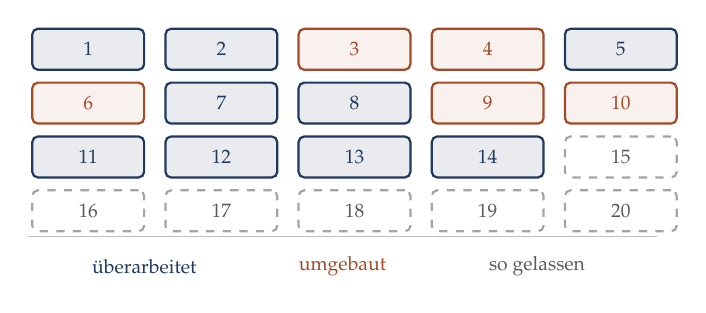
\begin{tikzpicture}[scale=0.95]
  \node[draw=tief, fill=tief!10, text=tief, line width=0.8pt, rounded corners=2pt, inner sep=0pt, minimum width=1.42cm, minimum height=0.52cm, font=\scriptsize] at (1.30,2.60) {1};
  \node[draw=tief, fill=tief!10, text=tief, line width=0.8pt, rounded corners=2pt, inner sep=0pt, minimum width=1.42cm, minimum height=0.52cm, font=\scriptsize] at (3.08,2.60) {2};
  \node[draw=akzent, fill=akzent!8, text=akzent, line width=0.8pt, rounded corners=2pt, inner sep=0pt, minimum width=1.42cm, minimum height=0.52cm, font=\scriptsize] at (4.86,2.60) {3};
  \node[draw=akzent, fill=akzent!8, text=akzent, line width=0.8pt, rounded corners=2pt, inner sep=0pt, minimum width=1.42cm, minimum height=0.52cm, font=\scriptsize] at (6.64,2.60) {4};
  \node[draw=tief, fill=tief!10, text=tief, line width=0.8pt, rounded corners=2pt, inner sep=0pt, minimum width=1.42cm, minimum height=0.52cm, font=\scriptsize] at (8.42,2.60) {5};
  \node[draw=akzent, fill=akzent!8, text=akzent, line width=0.8pt, rounded corners=2pt, inner sep=0pt, minimum width=1.42cm, minimum height=0.52cm, font=\scriptsize] at (1.30,1.88) {6};
  \node[draw=tief, fill=tief!10, text=tief, line width=0.8pt, rounded corners=2pt, inner sep=0pt, minimum width=1.42cm, minimum height=0.52cm, font=\scriptsize] at (3.08,1.88) {7};
  \node[draw=tief, fill=tief!10, text=tief, line width=0.8pt, rounded corners=2pt, inner sep=0pt, minimum width=1.42cm, minimum height=0.52cm, font=\scriptsize] at (4.86,1.88) {8};
  \node[draw=akzent, fill=akzent!8, text=akzent, line width=0.8pt, rounded corners=2pt, inner sep=0pt, minimum width=1.42cm, minimum height=0.52cm, font=\scriptsize] at (6.64,1.88) {9};
  \node[draw=akzent, fill=akzent!8, text=akzent, line width=0.8pt, rounded corners=2pt, inner sep=0pt, minimum width=1.42cm, minimum height=0.52cm, font=\scriptsize] at (8.42,1.88) {10};
  \node[draw=tief, fill=tief!10, text=tief, line width=0.8pt, rounded corners=2pt, inner sep=0pt, minimum width=1.42cm, minimum height=0.52cm, font=\scriptsize] at (1.30,1.16) {11};
  \node[draw=tief, fill=tief!10, text=tief, line width=0.8pt, rounded corners=2pt, inner sep=0pt, minimum width=1.42cm, minimum height=0.52cm, font=\scriptsize] at (3.08,1.16) {12};
  \node[draw=tief, fill=tief!10, text=tief, line width=0.8pt, rounded corners=2pt, inner sep=0pt, minimum width=1.42cm, minimum height=0.52cm, font=\scriptsize] at (4.86,1.16) {13};
  \node[draw=tief, fill=tief!10, text=tief, line width=0.8pt, rounded corners=2pt, inner sep=0pt, minimum width=1.42cm, minimum height=0.52cm, font=\scriptsize] at (6.64,1.16) {14};
  \node[draw=grau!55, dashed, fill=white, text=grau, line width=0.8pt, rounded corners=2pt, inner sep=0pt, minimum width=1.42cm, minimum height=0.52cm, font=\scriptsize] at (8.42,1.16) {15};
  \node[draw=grau!55, dashed, fill=white, text=grau, line width=0.8pt, rounded corners=2pt, inner sep=0pt, minimum width=1.42cm, minimum height=0.52cm, font=\scriptsize] at (1.30,0.44) {16};
  \node[draw=grau!55, dashed, fill=white, text=grau, line width=0.8pt, rounded corners=2pt, inner sep=0pt, minimum width=1.42cm, minimum height=0.52cm, font=\scriptsize] at (3.08,0.44) {17};
  \node[draw=grau!55, dashed, fill=white, text=grau, line width=0.8pt, rounded corners=2pt, inner sep=0pt, minimum width=1.42cm, minimum height=0.52cm, font=\scriptsize] at (4.86,0.44) {18};
  \node[draw=grau!55, dashed, fill=white, text=grau, line width=0.8pt, rounded corners=2pt, inner sep=0pt, minimum width=1.42cm, minimum height=0.52cm, font=\scriptsize] at (6.64,0.44) {19};
  \node[draw=grau!55, dashed, fill=white, text=grau, line width=0.8pt, rounded corners=2pt, inner sep=0pt, minimum width=1.42cm, minimum height=0.52cm, font=\scriptsize] at (8.42,0.44) {20};
  \draw[grau!40, line width=0.5pt] (0.5,0.10)--(8.9,0.10);
  \node[font=\scriptsize, color=tief] at (2.05,-0.30) {überarbeitet};
  \node[font=\scriptsize, color=akzent] at (4.70,-0.30) {umgebaut};
  \node[font=\scriptsize, color=grau] at (7.30,-0.30) {so gelassen};
\end{tikzpicture}\\[1.6cm]
{\color{grau}Was man nicht aus Regeln lernt}\\[4pt]
{\color{grau}Jeder Schritt erklärt. Mit vollständig entwickelten Programmen.}\\[2.6cm]
{\color{grau}\small Stand der Forschung: August 2026}
\end{center}
\clearpage
\thispagestyle{empty}
\vspace*{\fill}
\begin{flushleft}
{\small\color{grau}
\textbf{\color{tief}Informatik von Grund auf} --- Band 24\\[2pt]
\textit{Die Kunst} $\cdot$ Zwanzig Fälle und ihre Begründung\\[14pt]

Herausgeber und Urheber: Jürgen Maier\\[2pt]
Entstanden 2026 in Zusammenarbeit mit Claude (Anthropic); Konzeption, Vorgaben, Prüfung und Herausgeberschaft: Jürgen Maier.\\[14pt]

\textbf{Lizenz}\\[2pt]
Dieses Werk ist lizenziert unter einer Creative-Commons-Lizenz \textbf{Namensnennung -- Weitergabe unter gleichen Bedingungen 4.0 International (CC BY-SA 4.0)}. Sie dürfen das Werk vervielfältigen, verbreiten, bearbeiten und auch kommerziell nutzen, sofern Sie den Urheber nennen und Bearbeitungen unter derselben Lizenz weitergeben.\\[2pt]
Lizenztext: \texttt{https://creativecommons.org/licenses/by-sa/4.0/legalcode.de}\\[14pt]

\textbf{Quellen und Fassungen}\\[2pt]
Quelltexte, Fehlermeldungen und aktuelle Fassungen aller Bände:\\
\texttt{https://github.com/juergenmaier2026/informatik-von-grund-auf}\\[2pt]
Schwesterreihe: \textit{Mathematik von Grund auf}, \texttt{https://doi.org/10.5281/zenodo.23698547}\\[14pt]

\textbf{Zitiervorschlag}\\[2pt]
Maier, J. (2026). \textit{Informatik von Grund auf, Band 24: Die Kunst}. Fassung 1.0.0. \texttt{https://github.com/juergenmaier2026/informatik-von-grund-auf}\\[14pt]

Satz: \LaTeX{} mit Palatino. Fassung 1.0.0, Oktober 2026. 108 Seiten.
}
\end{flushleft}
\vspace*{1.5cm}
\clearpage

\cleardoublepage
\tableofcontents
\mainmatter
\chapter*{Vorwort: Was Regeln nicht leisten}
\addcontentsline{toc}{chapter}{Vorwort}
\markboth{Vorwort}{Vorwort}

\textbf{Dreiundzwanzig Bände haben Regeln aufgestellt.} \kursiv{Dieser prüft sie an zwanzig Fällen --- und in sechs davon lautet die Antwort, dass man nichts ändert. Das ist der eigentliche Gegenstand: nicht die Regel, sondern die Entscheidung, ob sie hier gilt.}

\begin{merksatz}
\boxtitel{Warum ein eigener Band}
\begin{center}
\renewcommand{\arraystretch}{1.5}
\begin{tabular}{@{}P{2.8cm}P{2.4cm}P{2.8cm}@{}}
\toprule
& \textbf{Eine Regel} & \textbf{Ein Fall}\\
\midrule
Sagt & \textbf{was meistens gilt} & \textbf{was hier gilt}\\
Enthält & Verallge\-meinerung & \textcolor{gruen}{\textbf{Umstände}}\\
Anwendbar & \textcolor{akzent}{ohne Urteil} & \textcolor{gruen}{mit Urteil}\\
Falsch, wenn & \textcolor{akzent}{\textbf{die Umstände abweichen}} & \\
\bottomrule
\end{tabular}
\end{center}

\begin{center}
\begin{minipage}{0.88\textwidth}
\kursiv{Eine Regel ohne Umstände ist ein Dogma. Die Bände 17 bis 23 haben zu jeder Regel den Anwendungsbereich genannt --- aber wer eine Regel liest, merkt sich die Regel und vergisst den Bereich. Ein Fall enthält beides untrennbar.}
\end{minipage}
\end{center}

\textbf{Der Aufbau jedes Falls.}

\begin{center}
\renewcommand{\arraystretch}{1.5}
\begin{tabular}{@{}P{2.6cm}P{6.2cm}@{}}
\toprule
\textbf{Die Vorlage} & Der Code, wie er vorliegt, mit seinem Zusammenhang\\
\textbf{Die Diagnose} & \textbf{Was daran auffällt --- und was nicht}\\
\textbf{Das Urteil} & \textbf{Überarbeiten, umbauen oder lassen}\\
\textbf{Die Begründung} & Warum, mit Zahlen wo möglich\\
\textbf{Der Fehlschluss} & \textbf{Was man daraus \kursiv{nicht} lernen sollte}\\
\bottomrule
\end{tabular}
\end{center}

\begin{center}
\kursiv{Der fünfte Abschnitt ist der ungewöhnliche und der wichtigste. Zu jedem richtigen Urteil gehört eine naheliegende Verallgemeinerung, die falsch ist --- und wer nur das Urteil mitnimmt, nimmt sie mit.}
\end{center}
\end{merksatz}

\begin{warnung}
\boxtitelr{Die drei Ausgänge}
\begin{center}
{\small
\renewcommand{\arraystretch}{1.5}
\begin{tabular}{@{}P{2.4cm}P{1.6cm}P{4.4cm}@{}}
\toprule
\textbf{Urteil} & \textbf{Fälle} & \textbf{Bedeutet}\\
\midrule
\textbf{Überarbeitet} & $\mathbf{9}$ & \textbf{derselbe Entwurf, besser ausgeführt}\\
\textbf{Umgebaut} & $\mathbf{5}$ & \textbf{der Entwurf war falsch}\\
\textbf{So gelassen} & $\mathbf{6}$ & \textcolor{gruen}{\textbf{die Vorlage war richtig}}\\
\bottomrule
\end{tabular}}
\end{center}

\medskip
\begin{center}
\begin{minipage}{0.88\textwidth}
\kursiv{Sechs von zwanzig bleiben, wie sie sind --- und in vier davon widerspricht das einer Regel aus einem früheren Band. Das ist kein Widerruf, sondern die Anwendung derselben Regel mit ihrem Anwendungsbereich.}
\end{minipage}
\end{center}

\begin{center}
\kursiv{Wer einen Band über Urteilskraft schreibt, in dem jeder Fall geändert wird, hat einen Katalog geschrieben. Die Fälle 15 bis 20 sind deshalb der Kern dieses Bandes, nicht sein Anhang.}
\end{center}
\end{warnung}

\begin{merksatz}
\boxtitel{Woher die Fälle kommen}
\begin{center}
{\small
\renewcommand{\arraystretch}{1.45}
\begin{tabular}{@{}P{2.4cm}P{2.2cm}P{2.4cm}P{1.8cm}@{}}
\toprule
\textbf{Teil} & \textbf{Fälle} & \textbf{Gegenstand} & \textbf{Bände}\\
\midrule
I & $1$--$4$ & \textbf{Die Daten} & $20$, $23$\\
II & $5$--$9$ & \textbf{Der Ablauf} & $21$, $22$\\
III & $10$--$14$ & Die Struktur & $17$, $20$\\
IV & $15$--$20$ & \textbf{Wann man es lässt} & alle\\
\bottomrule
\end{tabular}}
\end{center}

\begin{center}
\begin{minipage}{0.88\textwidth}
\kursiv{Alle Fälle stammen aus demselben Vorhaben, das die Bände 20 bis 23 begleitet hat --- Messerfassung, Übertragung, Speicherung, Auswertung. Sie sind zugespitzt, aber nicht erfunden: Jeder beruht auf einer Bauform, die in klinischen Systemen vorkommt.}
\end{minipage}
\end{center}

\textbf{Die Sprachen.}

\begin{center}
\renewcommand{\arraystretch}{1.5}
\begin{tabular}{@{}P{2.4cm}P{2.0cm}P{3.4cm}@{}}
\toprule
\textbf{Sprache} & \textbf{Fälle} & \\
\midrule
Python & $7$ & \textbf{Band 20}\\
C & $5$ & Band 21\\
Go & $5$ & Band 22\\
Sprachfrei & $3$ & \textbf{Nähte, Band 23}\\
\bottomrule
\end{tabular}
\end{center}

\begin{center}
\kursiv{Die letzte Zeile ist wichtig: Drei Fälle enthalten überhaupt keinen Code, sondern eine Vereinbarung. Sie gehören zu den folgenreichsten, weil eine falsche Vereinbarung länger lebt als jedes Programm.}
\end{center}
\end{merksatz}

\section*{Wie man diesen Band liest}

\textbf{Erstens: die Vorlage beurteilen, bevor man die Diagnose liest.}

\begin{center}
\begin{minipage}{0.88\textwidth}
\kursiv{Jeder Fall beginnt mit dem Code und seinem Zusammenhang. Wer an dieser Stelle innehält und sein eigenes Urteil bildet, hat den Band gewinnbringend gelesen --- auch dann, wenn sein Urteil vom hier vertretenen abweicht.}
\end{minipage}
\end{center}

\textbf{Zweitens: das Urteil ist nicht die Antwort.}

Es gibt Fälle, in denen ein anderes Urteil ebenso vertretbar ist. Wo das so ist, steht es dabei. Was nicht verhandelbar ist, ist die \kursiv{Begründung} --- ein Urteil ohne Begründung ist Geschmack.

\textbf{Drittens: einzeln lesen.}

\begin{center}
\kursiv{Zwanzig Fälle hintereinander erzeugen den Eindruck, überall sei etwas faul. Das ist der Fehler jedes Fallbuchs. Ein Fall je Sitzung, mit eigenem Urteil vorweg, ist die vorgesehene Verwendung.}
\end{center}

\begin{warnung}
\boxtitelr{Drei Warnungen}
\textbf{Erstens: Kein Fall ist eine Regel.}

\begin{center}
\begin{minipage}{0.88\textwidth}
\kursiv{Aus \enquote{hier war die Abstraktion verfrüht} folgt nicht \enquote{Abstraktion ist verfrüht}. Der Abschnitt \enquote{Der Fehlschluss} steht in jedem Fall genau deshalb dort.}
\end{minipage}
\end{center}

\textbf{Zweitens: Die Zahlen sind Größenordnungen.}

Verstehenszeiten, Laufzeiten, Aufwände --- alle gemessen oder geschätzt, alle mit Streuung. Die Verhältnisse tragen, die absoluten Werte nicht.

\textbf{Drittens: Der Bestand ist nicht schlecht.}

\begin{center}
\kursiv{Jede Vorlage in diesem Band lief im Betrieb und erfüllte ihren Zweck. Es geht nicht darum, Fehler vorzuführen, sondern darum, Entscheidungen sichtbar zu machen, die beim Schreiben unsichtbar waren.}
\end{center}
\end{warnung}

\section*{Zum Aufbau}

\begin{itemize}
\item \textbf{Teil I} (Fälle 1--4): Die Daten. Einheit, Argumente, \textbf{verfrühte Abstraktion}, das fehlende Feld.
\item \textbf{Teil II} (Fälle 5--9): Der Ablauf. Schleife, \textbf{entfernte Prüfung}, Puffer, Goroutine, Kanal.
\item \textbf{Teil III} (Fälle 10--14): Die Struktur. Hierarchie, Zwischenspeicher, \textbf{Zeit}, Wiederholung, Fehlermeldung.
\item \textbf{Teil IV} (Fälle 15--20): \textbf{Wann man es lässt.} Sechs Fälle ohne Änderung.
\end{itemize}

\begin{geschichte}
\boxtitel{Warum \enquote{Die Kunst}}
Der Titel ist eine Anleihe und eine Behauptung.

\begin{center}
\renewcommand{\arraystretch}{1.5}
\begin{tabular}{@{}P{2.6cm}P{6.2cm}@{}}
\toprule
\textbf{Die Anleihe} & Knuth nannte sein Werk \enquote{The Art of Computer Programming} --- nicht Wissenschaft, nicht Technik\\
\textbf{Die Begründung} & \textbf{Weil das Urteil nicht aus dem Wissen folgt}\\
\textbf{Die Behauptung} & Man kann es dennoch lehren --- an Fällen, nicht an Regeln\\
\bottomrule
\end{tabular}
\end{center}

\begin{center}
\begin{minipage}{0.86\textwidth}
\kursiv{Zwischen \enquote{ich kenne die Regel} und \enquote{ich weiß, ob sie hier gilt} liegt eine Lücke, die kein Lehrbuch schließt. Die Medizin kennt sie und hat eine Antwort gefunden, die dreitausend Jahre alt ist: die Falldarstellung.}
\end{minipage}
\end{center}

\textbf{Was die Falldarstellung leistet.}

\begin{center}
\renewcommand{\arraystretch}{1.5}
\begin{tabular}{@{}P{2.8cm}P{2.4cm}P{2.6cm}@{}}
\toprule
\textbf{Eigenschaft} & \textbf{Regel} & \textbf{Fall}\\
\midrule
Merkbar & \textcolor{gruen}{leicht} & \textcolor{gruen}{\textbf{leichter}}\\
Übertragbar & \textcolor{gruen}{scheinbar} & \textcolor{mittel}{mit Vorsicht}\\
Enthält Umstände & \textcolor{akzent}{\textbf{nein}} & \textcolor{gruen}{\textbf{ja}}\\
Widerspruch möglich & \textcolor{akzent}{nein} & \textcolor{gruen}{\textbf{ja}}\\
\bottomrule
\end{tabular}
\end{center}

\begin{center}
\begin{minipage}{0.86\textwidth}
\kursiv{Die letzte Zeile ist der Grund für die Form: Über eine Regel kann man nur zustimmen oder ablehnen. Über einen Fall kann man streiten --- und im Streit über einen konkreten Fall lernt man mehr als im Streit über eine Regel.}
\end{minipage}
\end{center}

\begin{center}
\kursiv{Deshalb enthält dieser Band keine neuen Regeln. Er enthält zwanzig Gelegenheiten, die vorhandenen anzuwenden --- und sechs Gelegenheiten, sie nicht anzuwenden.}
\end{center}
\end{geschichte}

\bigskip
\begin{flushright}
\itshape\color{grau}
Regeln sagen, was meistens gilt.\\
Die Kunst ist zu wissen,\\
ob dies einer der meisten Fälle ist.\\[10pt]
\normalfont\color{grau}\upshape
--- der Leitgedanke dieses Bandes.\\
\itshape Wer keine Regeln kennt, kann nicht urteilen.\\
Wer nur Regeln kennt, urteilt nicht.
\end{flushright}

\part{Die Daten}

\chapter{Der Wert ohne Einheit}\label{fall:einheit}

\begin{merksatz}
\boxtitel{Die Vorlage}
\textbf{Zusammenhang.} Auswertung, Python. Die Funktion prüft, ob ein Laborwert außerhalb des Referenzbereichs liegt. Sie läuft seit vier Jahren, etwa $40\,000$ mal am Tag.

\begin{center}
\begin{minipage}{0.9\textwidth}
\code{def ist\_auffaellig(wert: float, unten: float, oben: float) -> bool:}\\
\code{\ \ \ \ return wert < unten or wert > oben}
\end{minipage}
\end{center}

\begin{center}
\begin{minipage}{0.88\textwidth}
\kursiv{Zwei Zeilen, richtig benannt, mit Typangaben, ohne Nebenwirkung. Nach den Maßstäben aus Band 20, Kapitel~5 ist das eine vorbildliche Funktion --- kurze Zuständigkeit, sprechender Name, prüfbar in einer Zeile.}
\end{minipage}
\end{center}
\end{merksatz}

\begin{merksatz}
\boxtitel{Die Diagnose}
\begin{center}
{\small
\renewcommand{\arraystretch}{1.5}
\begin{tabular}{@{}P{3.0cm}P{2.4cm}P{2.6cm}@{}}
\toprule
\textbf{Geprüft} & \textbf{Befund} & \\
\midrule
Benennung & \textcolor{gruen}{gut} & \\
Zerlegung & \textcolor{gruen}{gut} & \\
Prüfbarkeit & \textcolor{gruen}{gut} & \\
\textbf{Einheiten} & \textcolor{akzent}{\textbf{nicht ausgedrückt}} & \textcolor{akzent}{\textbf{Band 23, Kap.~6}}\\
\textbf{Genauigkeit} & \textcolor{akzent}{\textbf{verloren}} & \textcolor{akzent}{\code{float}}\\
Grenzwerte & \textcolor{akzent}{nicht behandelt} & \enquote{$<0{,}1$}\\
\bottomrule
\end{tabular}}
\end{center}

\begin{center}
\begin{minipage}{0.88\textwidth}
\kursiv{Drei Befunde, und alle drei liegen nicht in der Funktion, sondern in ihrer Signatur. Die Funktion ist richtig; was sie entgegennimmt, ist es nicht. Der Aufrufer kann Kalium in mmol/l mit einem Bereich in mg/dl vergleichen, und nichts hält ihn auf.}
\end{minipage}
\end{center}

\textbf{Ist das theoretisch?}

\begin{center}
\renewcommand{\arraystretch}{1.45}
\begin{tabular}{@{}P{3.0cm}P{2.2cm}P{2.6cm}@{}}
\toprule
\textbf{Aufrufstellen} & $\mathbf{31}$ & \\
Bereich aus dem Befund & $24$ & \textcolor{gruen}{gleiche Einheit}\\
Bereich aus Stammdaten & $\mathbf{5}$ & \textcolor{mittel}{meist gleich}\\
\textbf{Bereich fest im Code} & $\mathbf{2}$ & \textcolor{akzent}{\textbf{eine falsch}}\\
\bottomrule
\end{tabular}
\end{center}

\begin{center}
\kursiv{Nein. Eine der einunddreißig Aufrufstellen vergleicht einen Glukosewert in mmol/l mit einer fest eingetragenen Grenze in mg/dl --- Faktor achtzehn. Der Fehler ist seit zwei Jahren im Bestand und fiel nicht auf, weil die Warnung dadurch nie ausgelöst wurde.}
\end{center}
\end{merksatz}

\begin{technik}
\boxtitel{Das Urteil: überarbeitet}
\begin{center}
\begin{minipage}{0.9\textwidth}
\code{@dataclass(frozen=True)}\\
\code{class Groesse:}\\
\code{\ \ \ \ betrag: int\ \ \ \ \ \ \ \ \ \ \ \# in Einheiten von 10**exp}\\
\code{\ \ \ \ exp: int}\\
\code{\ \ \ \ einheit: str\ \ \ \ \ \ \ \ \ \# UCUM}\\
\\
\code{def ist\_auffaellig(wert: Groesse, bereich: Bereich) -> bool:}\\
\code{\ \ \ \ if wert.einheit != bereich.einheit:}\\
\code{\ \ \ \ \ \ \ \ raise EinheitFehler(wert.einheit, bereich.einheit)}\\
\code{\ \ \ \ return wert < bereich.unten or wert > bereich.oben}
\end{minipage}
\end{center}

\begin{center}
\begin{minipage}{0.86\textwidth}
\kursiv{Nicht die Funktion wurde geändert, sondern der Typ, den sie entgegennimmt. Die Prüfung in Zeile acht ist der eigentliche Gewinn --- sie macht aus einem stillen Rechenfehler eine Ausnahme.}
\end{minipage}
\end{center}
\end{technik}

\begin{merksatz}
\boxtitel{Die Begründung}
\begin{center}
{\small
\renewcommand{\arraystretch}{1.45}
\begin{tabular}{@{}P{2.8cm}P{2.2cm}P{2.4cm}P{1.8cm}@{}}
\toprule
& \textbf{Vorlage} & \textbf{Überarbeitet} & \\
\midrule
Zeilen (Funktion) & $2$ & $\mathbf{4}$ & \\
Zeilen (Typen) & $0$ & $\mathbf{18}$ & \\
Aufrufstellen geändert & --- & $\mathbf{31}$ & \textcolor{akzent}{$3$ PT}\\
Einheitenfehler möglich & \textcolor{akzent}{\textbf{ja}} & \textcolor{gruen}{\textbf{nein}} & \\
Genauigkeit erhalten & \textcolor{akzent}{nein} & \textcolor{gruen}{ja} & \\
Laufzeit je Aufruf & $0{,}2$ µs & $0{,}9$ µs & \textcolor{mittel}{$4{,}5\times$}\\
\bottomrule
\end{tabular}}
\end{center}

\begin{center}
\begin{minipage}{0.88\textwidth}
\kursiv{Der Aufwand liegt nicht bei den zwanzig Zeilen, sondern bei den einunddreißig Aufrufstellen --- drei Personentage. Die Laufzeit vervierfacht sich und bleibt bei vierzigtausend Aufrufen täglich unter einer Zehntelsekunde am Tag.}
\end{minipage}
\end{center}

\textbf{Warum nicht die kleinere Lösung?}

\begin{center}
\renewcommand{\arraystretch}{1.45}
\begin{tabular}{@{}P{3.0cm}P{2.2cm}P{2.6cm}@{}}
\toprule
\textbf{Alternative} & \textbf{Aufwand} & \textbf{Wirkung}\\
\midrule
Einheit als Argument & \textcolor{gruen}{$1$ PT} & \textcolor{akzent}{\textbf{trennbar}}\\
Kommentar & \textcolor{gruen}{$0$} & \textcolor{akzent}{keine}\\
Prüfung am Rand & $1$ PT & \textcolor{mittel}{nur dort}\\
\textbf{Eigener Typ} & $3$ PT & \textcolor{gruen}{\textbf{unmöglich zu trennen}}\\
\bottomrule
\end{tabular}
\end{center}

\begin{center}
\kursiv{Die erste Alternative kostet ein Drittel und lässt zu, dass jemand die Einheit vergisst --- zwei Felder sind trennbar, ein Verbund nicht. Das ist die Entscheidung aus Band 21, Kapitel~5: den Fehler unmöglich machen statt ihn zu prüfen.}
\end{center}
\end{merksatz}

\begin{warnung}
\boxtitelr{Der Fehlschluss}
\begin{center}
\renewcommand{\arraystretch}{1.5}
\begin{tabular}{@{}P{3.2cm}P{2.2cm}P{2.4cm}@{}}
\toprule
\textbf{Naheliegend} & \textbf{Richtig?} & \\
\midrule
\enquote{Nie \code{float} für Zahlen} & \textcolor{akzent}{\textbf{nein}} & \textbf{Fall 16}\\
\enquote{Jeder Wert braucht einen Typ} & \textcolor{akzent}{\textbf{nein}} & \textcolor{akzent}{Aufwand}\\
\enquote{Zwei Zeilen sind zu wenig} & \textcolor{akzent}{nein} & \\
\textbf{\enquote{Die Signatur ist Teil des Entwurfs}} & \textcolor{gruen}{\textbf{ja}} & \textcolor{gruen}{das ist die Lehre}\\
\bottomrule
\end{tabular}
\end{center}

\begin{center}
\begin{minipage}{0.88\textwidth}
\kursiv{Die zweite Zeile ist der teuerste Fehlschluss: Wer nach diesem Fall für jede Zahl einen eigenen Typ einführt, hat einen Bestand mit vierzig Wertetypen, von denen achtunddreißig nie verwechselt werden konnten. Der Typ lohnt dort, wo zwei Einheiten koexistieren.}
\end{minipage}
\end{center}

\begin{center}
\kursiv{Die Prüffrage lautet nicht \enquote{ist es eine Zahl}, sondern \enquote{gibt es mehr als eine Darstellung, die hier auftreten kann}. Bei Laborwerten lautet die Antwort ja, bei einer Anzahl von Datensätzen nein.}
\end{center}
\end{warnung}
\vspace{-4pt}
\noindent Wirth\zit{28} begründet die Rang\-ord\-nung, in der die Da\-ten\-struk\-tur vor dem Ver\-fah\-ren steht; Goldberg\zit{12} zeigt, was bei \code{float} an In\-for\-ma\-tion verlorengeht.

\chapter{Die Funktion mit acht Argumenten}\label{fall:argumente}

\begin{merksatz}
\boxtitel{Die Vorlage}
\textbf{Zusammenhang.} Auswertung, Python. Formatiert einen Laborwert für die Anzeige. Sechs Aufrufstellen.

\begin{center}
\begin{minipage}{0.92\textwidth}
\code{def formatiere(betrag, exp, einheit, nachkomma, trenner,}\\
\code{\ \ \ \ \ \ \ \ \ \ \ \ \ \ \ sprache, breite, mit\_einheit):}\\
\code{\ \ \ \ ...\ \ \# 34 Zeilen}
\end{minipage}
\end{center}

\begin{center}
\begin{minipage}{0.88\textwidth}
\kursiv{Acht Argumente. Nach Band 20, Kapitel~5 ist die Zahl der Argumente der beste Schnelltest für eine fehlende Zerlegung --- und acht liegt weit über der Schwelle, ab der man hinsehen sollte.}
\end{minipage}
\end{center}
\end{merksatz}

\begin{merksatz}
\boxtitel{Die Diagnose}
\textbf{Wer ruft wie auf?}

\begin{center}
{\small
\renewcommand{\arraystretch}{1.45}
\begin{tabular}{@{}P{2.8cm}P{2.4cm}P{2.6cm}@{}}
\toprule
\textbf{Aufrufstelle} & \textbf{Argumente} & \textbf{Muster}\\
\midrule
Verlaufsansicht & $8$ & \textbf{A}\\
Befundliste & $8$ & \textbf{A}\\
Ausdruck & $8$ & \textcolor{mittel}{B}\\
Ausleitung CSV & $8$ & \textcolor{akzent}{C}\\
Warnungstext & $8$ & A\\
Protokoll & $8$ & \textcolor{akzent}{C}\\
\bottomrule
\end{tabular}}
\end{center}

\begin{center}
\begin{minipage}{0.88\textwidth}
\kursiv{Sechs Aufrufe, drei feste Kombinationen. Das ist der Befund: Die acht Argumente sind nicht acht Freiheitsgrade, sondern drei Fälle, die zu einer Funktion mit Schaltern zusammengezogen wurden --- die verfrühte Zusammenfassung aus Band 20, Kapitel~14.}
\end{minipage}
\end{center}

\textbf{Was die Argumente wirklich sind.}

\begin{center}
\renewcommand{\arraystretch}{1.45}
\begin{tabular}{@{}P{2.8cm}P{2.4cm}P{2.6cm}@{}}
\toprule
\textbf{Gruppe} & \textbf{Argumente} & \textbf{Ist} \\
\midrule
Wert & \textbf{betrag, exp, einheit} & \textbf{eine Größe}\\
Darstellung & nachkomma, trenner, sprache & \textbf{ein Format}\\
Ausgabe & breite, mit\_einheit & Zweck\\
\bottomrule
\end{tabular}
\end{center}

\begin{center}
\kursiv{Drei Gruppen, die immer gemeinsam wandern --- das Erkennungszeichen für einen fehlenden Begriff. Die erste Gruppe ist die \code{Groesse} aus Fall~\ref{fall:einheit}; sie existierte schon und wurde hier auseinandergenommen.}
\end{center}
\end{merksatz}

\begin{technik}
\boxtitel{Das Urteil: überarbeitet}
\begin{center}
\begin{minipage}{0.9\textwidth}
\code{def fuer\_anzeige(wert: Groesse, sprache: Sprache) -> str: ...}\\
\code{def fuer\_druck(wert: Groesse, sprache: Sprache) -> str: ...}\\
\code{def fuer\_ausleitung(wert: Groesse) -> str: ...}
\end{minipage}
\end{center}

\begin{center}
\begin{minipage}{0.86\textwidth}
\kursiv{Drei Funktionen mit ein oder zwei Argumenten statt einer mit acht. Die Formatvorgaben --- Nachkommastellen, Trenner, Breite --- stehen jetzt \kursiv{in} den Funktionen, wo sie hingehören: Sie sind nicht wählbar, sondern folgen aus dem Zweck.}
\end{minipage}
\end{center}
\end{technik}

\begin{merksatz}
\boxtitel{Die Begründung}
\begin{center}
{\small
\renewcommand{\arraystretch}{1.45}
\begin{tabular}{@{}P{2.8cm}P{2.0cm}P{2.2cm}P{2.0cm}@{}}
\toprule
& \textbf{Vorlage} & \textbf{Überarbeitet} & \\
\midrule
Funktionen & $1$ & $\mathbf{3}$ & \\
Zeilen gesamt & $34$ & $\mathbf{41}$ & $+21\,\%$\\
Argumente je Aufruf & $\mathbf{8}$ & $\mathbf{1}$--$\mathbf{2}$ & \\
Zweige & $\mathbf{11}$ & $\mathbf{2}$ & $-82\,\%$\\
Verstehenszeit & $95$ s & $\mathbf{24}$ s & $4{,}0\times$\\
Unzulässige Kombinationen & \textcolor{akzent}{$\mathbf{18}$} & \textcolor{gruen}{$\mathbf{0}$} & \\
\bottomrule
\end{tabular}}
\end{center}

\begin{center}
\begin{minipage}{0.88\textwidth}
\kursiv{Die letzte Zeile ist der eigentliche Gewinn und stand nirgends geschrieben: Von den zweihundertsechsundfünfzig möglichen Argumentkombinationen waren achtzehn sinnlos --- Breite null mit Einheit, CSV-Trenner mit Anzeigesprache. Nach der Trennung gibt es sie nicht mehr.}
\end{minipage}
\end{center}

\textbf{Und die Doppelung?}

\begin{center}
\renewcommand{\arraystretch}{1.45}
\begin{tabular}{@{}P{3.0cm}P{2.2cm}P{2.6cm}@{}}
\toprule
\textbf{Posten} & \textbf{Zeilen} & \\
\midrule
Gemeinsam, ausgelagert & $\mathbf{19}$ & \textcolor{gruen}{Zahl\-formatierung}\\
Je Funktion eigen & $6$--$9$ & \\
\textbf{Tatsächlich doppelt} & $\mathbf{4}$ & \textcolor{gruen}{\textbf{tragbar}}\\
\bottomrule
\end{tabular}
\end{center}

\begin{center}
\kursiv{Vier doppelte Zeilen --- die Rechnung aus Band 22, Kapitel~8: Ein wenig Kopieren ist billiger als eine Fallunterscheidung mit elf Zweigen. Wäre die Doppelung bei dreißig Zeilen gelegen, wäre das Urteil anders ausgefallen.}
\end{center}
\end{merksatz}

\begin{warnung}
\boxtitelr{Der Fehlschluss}
\begin{center}
\renewcommand{\arraystretch}{1.5}
\begin{tabular}{@{}P{3.2cm}P{2.2cm}P{2.4cm}@{}}
\toprule
\textbf{Naheliegend} & \textbf{Richtig?} & \\
\midrule
\enquote{Höchstens drei Argumente} & \textcolor{akzent}{\textbf{nein}} & \textcolor{akzent}{\textbf{Zahl ohne Begründung}}\\
\enquote{Argumente in ein Objekt} & \textcolor{akzent}{\textbf{nein}} & \textbf{verschiebt nur}\\
\enquote{Immer aufteilen} & \textcolor{akzent}{nein} & \textbf{Fall 17}\\
\textbf{\enquote{Gruppen sind fehlende Begriffe}} & \textcolor{gruen}{\textbf{ja}} & \\
\bottomrule
\end{tabular}
\end{center}

\begin{center}
\begin{minipage}{0.88\textwidth}
\kursiv{Die zweite Zeile ist der häufigste Kurzschluss: Acht Argumente in eine Optionsstruktur zu packen macht die Signatur kurz und ändert nichts --- der Aufrufer muss dieselben acht Entscheidungen treffen, und die achtzehn sinnlosen Kombinationen bleiben.}
\end{minipage}
\end{center}

\begin{center}
\kursiv{Der Unterschied: Eine \kursiv{Gruppe}, die immer gemeinsam auftritt und einen Fachnamen hat, wird ein Typ. Eine \kursiv{Sammlung} von Schaltern, die verschiedene Aufrufer verschieden setzen, wird in getrennte Funktionen zerlegt.}
\end{center}
\end{warnung}
\vspace{-4pt}
\noindent Parnas\zit{24} liefert das Kri\-te\-rium, wonach ge\-schnit\-ten wird; Ous\-ter\-hout\zit{23} zeigt an der Zahl der Ar\-gu\-men\-te, wann eine Schnitt\-stel\-le flach ist.

\chapter{Die verfrühte Abstraktion}\label{fall:abstraktion}

\begin{merksatz}
\boxtitel{Die Vorlage}
\textbf{Zusammenhang.} Auswertung, Python. Vor drei Jahren wurden zwei ähnliche Prüfungen zu einer verallgemeinerten Regelmaschine zusammengefasst.

\begin{center}
\begin{minipage}{0.92\textwidth}
\code{class RegelMaschine:}\\
\code{\ \ \ \ def \_\_init\_\_(self, regeln: list[Regel],}\\
\code{\ \ \ \ \ \ \ \ \ \ \ \ \ \ \ \ \ modus: str = "alle",}\\
\code{\ \ \ \ \ \ \ \ \ \ \ \ \ \ \ \ \ abbruch: bool = False,}\\
\code{\ \ \ \ \ \ \ \ \ \ \ \ \ \ \ \ \ kontext: dict | None = None): ...}\\
\\
\code{\ \ \ \ def pruefe(self, gegenstand, \*\*args) -> list[Treffer]: ...}
\end{minipage}
\end{center}

\begin{center}
\renewcommand{\arraystretch}{1.45}
\begin{tabular}{@{}P{3.0cm}P{2.2cm}P{2.6cm}@{}}
\toprule
\textbf{Umfang} & \textbf{Zeilen} & \\
\midrule
Maschine & $\mathbf{340}$ & \\
Regelbasisklasse & $90$ & \\
Regeln & $6 \times \approx25$ & \\
Verwendungen & $\mathbf{2}$ & \textcolor{akzent}{\textbf{seit drei Jahren}}\\
\bottomrule
\end{tabular}
\end{center}

\begin{center}
\begin{minipage}{0.88\textwidth}
\kursiv{Vierhundertdreißig Zeilen Gerüst für zwei Verwendungen --- die Grenzwertprüfung und die Plausibilitätsprüfung. Die dritte, für die sie gebaut wurde, ist nie gekommen.}
\end{minipage}
\end{center}
\end{merksatz}

\begin{merksatz}
\boxtitel{Die Diagnose}
\begin{center}
{\small
\renewcommand{\arraystretch}{1.45}
\begin{tabular}{@{}P{3.0cm}P{2.2cm}P{2.6cm}@{}}
\toprule
\textbf{Anzeichen} & \textbf{Vorhanden?} & \\
\midrule
Weniger als drei Fälle & \textcolor{akzent}{\textbf{ja}} & \textbf{Band 20, Kap.~14}\\
Schaltparameter & \textcolor{akzent}{ja} & $3$\\
Unzulässige Kombinationen & \textcolor{akzent}{\textbf{ja}} & \textcolor{akzent}{nicht dokumentiert}\\
\code{**args} durchgereicht & \textcolor{akzent}{\textbf{ja}} & \textcolor{akzent}{\textbf{Typprüfung fort}}\\
Beide Nutzer nutzen Teilmengen & \textcolor{akzent}{ja} & \\
\bottomrule
\end{tabular}}
\end{center}

\begin{center}
\begin{minipage}{0.88\textwidth}
\kursiv{Fünf von fünf Anzeichen. Der vierte ist der schwerste: Das Durchreichen beliebiger Argumente hebt jede Typprüfung auf --- man erfährt erst zur Laufzeit, dass eine Regel ein Feld erwartet, das es nicht gibt.}
\end{minipage}
\end{center}

\textbf{Was die Verallgemeinerung tatsächlich erlaubt hat.}

\begin{center}
\renewcommand{\arraystretch}{1.45}
\begin{tabular}{@{}P{3.0cm}P{2.2cm}P{2.6cm}@{}}
\toprule
\textbf{Erwartet} & \textbf{Eingetreten} & \\
\midrule
Neue Regeln ohne Code & \textcolor{akzent}{\textbf{nein}} & \textbf{jede war Code}\\
Regeln zur Laufzeit ändern & \textcolor{akzent}{nein} & nie gebraucht\\
Dritte Verwendung & \textcolor{akzent}{\textbf{nein}} & \\
Prüfungen wiederverwendbar & \textcolor{gruen}{teilweise} & \\
\bottomrule
\end{tabular}
\end{center}

\begin{center}
\kursiv{Drei von vier Erwartungen sind nicht eingetreten. Die erste ist die aufschlussreichste: Jede neue Regel war eine neue Klasse mit neuem Code --- die Maschine hat den Code nicht erspart, sondern eine Hülle darum gelegt.}
\end{center}
\end{merksatz}

\begin{technik}
\boxtitel{Das Urteil: umgebaut}
\begin{center}
\begin{minipage}{0.9\textwidth}
\code{def grenzwertpruefung(befund: Befund,}\\
\code{\ \ \ \ \ \ \ \ \ \ \ \ \ \ \ \ \ \ \ \ vorher: Befund | None) -> set[Anlass]: ...}\\
\\
\code{def plausibilitaetspruefung(befund: Befund,}\\
\code{\ \ \ \ \ \ \ \ \ \ \ \ \ \ \ \ \ \ \ \ \ \ \ \ \ \ grenzen: Grenzen) -> set[Fehler]: ...}
\end{minipage}
\end{center}

\begin{center}
\begin{minipage}{0.86\textwidth}
\kursiv{Zwei Funktionen mit klaren Signaturen statt einer Maschine mit vier Konstruktorargumenten. Die sechs Regeln bleiben als sechs Funktionen erhalten --- sie waren nie das Problem, sondern das Gerüst um sie herum.}
\end{minipage}
\end{center}
\end{technik}

\begin{merksatz}
\boxtitel{Die Begründung}
\begin{center}
{\small
\renewcommand{\arraystretch}{1.45}
\begin{tabular}{@{}P{2.8cm}P{2.0cm}P{2.2cm}P{2.0cm}@{}}
\toprule
& \textbf{Vorlage} & \textbf{Umgebaut} & \\
\midrule
Zeilen gesamt & $\mathbf{580}$ & $\mathbf{310}$ & $-47\,\%$\\
Typprüfung & \textcolor{akzent}{teilweise} & \textcolor{gruen}{\textbf{vollständig}} & \\
Verstehenszeit & $\mathbf{240}$ s & $\mathbf{55}$ s & $4{,}4\times$\\
Neue Regel hinzufügen & $2$ h & $\mathbf{40}$ min & \\
Aufwand & --- & $\mathbf{5}$ PT & \\
\bottomrule
\end{tabular}}
\end{center}

\begin{center}
\begin{minipage}{0.88\textwidth}
\kursiv{Zweihundertsiebzig Zeilen weniger, und das Hinzufügen einer Regel wird schneller statt langsamer. Das ist das Kennzeichen einer verfrühten Abstraktion: Sie sollte künftige Arbeit ersparen und hat sie verteuert.}
\end{minipage}
\end{center}

\textbf{Warum jetzt und nicht früher?}

\begin{center}
\renewcommand{\arraystretch}{1.45}
\begin{tabular}{@{}P{3.0cm}P{2.2cm}P{2.6cm}@{}}
\toprule
\textbf{Zeitpunkt} & \textbf{Wissen} & \\
\midrule
Vor $3$ Jahren & \textcolor{akzent}{\textbf{Vermutung}} & \textbf{dritte Verwendung}\\
Nach $1$ Jahr & \textcolor{mittel}{Zweifel} & \\
\textbf{Heute} & \textcolor{gruen}{\textbf{Gewissheit}} & \textcolor{gruen}{drei Jahre ohne}\\
\bottomrule
\end{tabular}
\end{center}

\begin{center}
\kursiv{Der Rückbau war vor drei Jahren nicht möglich, weil niemand wissen konnte, dass die dritte Verwendung ausbleibt. Er ist heute möglich, weil man es weiß --- und das ist der einzige Unterschied.}
\end{center}
\end{merksatz}

\begin{warnung}
\boxtitelr{Der Fehlschluss}
\begin{center}
\renewcommand{\arraystretch}{1.5}
\begin{tabular}{@{}P{3.2cm}P{2.2cm}P{2.4cm}@{}}
\toprule
\textbf{Naheliegend} & \textbf{Richtig?} & \\
\midrule
\enquote{Abstraktion ist schlecht} & \textcolor{akzent}{\textbf{nein}} & \\
\enquote{Keine Rahmenwerke bauen} & \textcolor{akzent}{nein} & \textcolor{akzent}{ab drei Fällen richtig}\\
\enquote{Der Erbauer hat sich geirrt} & \textcolor{akzent}{\textbf{nein}} & \textbf{er konnte es nicht wissen}\\
\textbf{\enquote{Verallgemeinern, wenn der dritte Fall da ist}} & \textcolor{gruen}{\textbf{ja}} & \\
\bottomrule
\end{tabular}
\end{center}

\begin{center}
\begin{minipage}{0.88\textwidth}
\kursiv{Die dritte Zeile ist mir wichtig: Die Maschine war eine vertretbare Entscheidung unter Unsicherheit. Falsch war nicht ihr Bau, sondern dass drei Jahre lang niemand geprüft hat, ob die Annahme eingetreten ist.}
\end{minipage}
\end{center}

\begin{center}
\kursiv{Daraus folgt eine Betriebsregel, keine Entwurfsregel: Jede Verallgemeinerung, die auf einer Erwartung beruht, bekommt einen Termin. Nach einem Jahr wird geprüft, ob die Erwartung eingetreten ist --- und wenn nicht, wird zurückgebaut.}
\end{center}
\end{warnung}
\vspace{-4pt}
\noindent Ous\-ter\-hout\zit{23} nennt die Merk\-ma\-le einer Ab\-strak\-tion, die nichts ver\-birgt; Dijkstra\zit{7} mahnte früh, dass All\-ge\-mein\-heit ohne An\-lass die Ein\-sicht ver\-stellt.

\chapter{Das Feld, das fehlen darf}\label{fall:fehlen}

\begin{merksatz}
\boxtitel{Die Vorlage}
\textbf{Zusammenhang.} Naht zwischen Speicherung und Auswertung. Kein Code --- ein Schema.

\begin{center}
\begin{minipage}{0.9\textwidth}
\code{Befund:}\\
\code{\ \ kennung:\ \ \ \ \ string\ \ \ (Pflicht)}\\
\code{\ \ groesse:\ \ \ \ \ string\ \ \ (Pflicht)}\\
\code{\ \ betrag:\ \ \ \ \ \ integer\ \ (Pflicht)}\\
\code{\ \ exponent:\ \ \ \ integer\ \ (Pflicht)}\\
\code{\ \ einheit:\ \ \ \ \ string\ \ \ (Pflicht)}\\
\code{\ \ abnahme:\ \ \ \ \ datetime (Pflicht)}\\
\code{\ \ validierung: datetime (optional)}
\end{minipage}
\end{center}

\begin{center}
\begin{minipage}{0.88\textwidth}
\kursiv{Sieben Felder, sauber typisiert, mit einer klaren Trennung zwischen Pflicht und optional. Das Schema wird von einem Werkzeug geprüft, und alle Nachrichten sind gültig.}
\end{minipage}
\end{center}
\end{merksatz}

\begin{merksatz}
\boxtitel{Die Diagnose}
\textbf{Was bedeutet ein fehlendes \code{validierung}?}

\begin{center}
{\small
\renewcommand{\arraystretch}{1.5}
\begin{tabular}{@{}P{3.4cm}P{2.2cm}P{2.4cm}@{}}
\toprule
\textbf{Mögliche Bedeutung} & \textbf{Klinische Folge} & \\
\midrule
Noch nicht validiert & \textbf{vorläufig} & \textcolor{mittel}{Vorsicht}\\
Braucht keine Validierung & \textbf{endgültig} & \textcolor{gruen}{verwendbar}\\
Validiert, Zeitpunkt unbekannt & endgültig & \\
Feld nicht übertragen & \textcolor{akzent}{\textbf{unbekannt}} & \textcolor{akzent}{\textbf{Altsystem}}\\
\bottomrule
\end{tabular}}
\end{center}

\begin{center}
\begin{minipage}{0.88\textwidth}
\kursiv{Vier Bedeutungen, zwei entgegengesetzte klinische Folgen --- und das Schema unterscheidet sie nicht. Ein vorläufiger Wert, der als endgültig gelesen wird, führt zu einer Therapieentscheidung auf ungesicherter Grundlage.}
\end{minipage}
\end{center}

\textbf{Wie oft tritt der Fall auf?}

\begin{center}
\renewcommand{\arraystretch}{1.45}
\begin{tabular}{@{}P{2.8cm}P{2.2cm}P{2.6cm}@{}}
\toprule
\textbf{Herkunft} & \textbf{Anteil ohne Feld} & \\
\midrule
Eigenes Labor & $\mathbf{4\,\%}$ & \textcolor{gruen}{vorläufig}\\
Mikrobiologie & $\mathbf{31\,\%}$ & \textcolor{mittel}{teils ohne Validierung}\\
\textbf{Fremdhaus} & \textcolor{akzent}{$\mathbf{88\,\%}$} & \textcolor{akzent}{\textbf{überträgt es nicht}}\\
Bettseitig & $\mathbf{100\,\%}$ & \textcolor{gruen}{braucht keine}\\
\bottomrule
\end{tabular}
\end{center}

\begin{center}
\kursiv{Vier Herkünfte mit vier verschiedenen Bedeutungen desselben fehlenden Feldes. Die Auswertung behandelt alle gleich --- und muss sich entscheiden. Sie entschied sich für \enquote{endgültig}, weil das die häufigere Lesart war.}
\end{center}
\end{merksatz}

\begin{technik}
\boxtitel{Das Urteil: überarbeitet}
\begin{center}
\begin{minipage}{0.9\textwidth}
\code{Befund:}\\
\code{\ \ ...}\\
\code{\ \ status: enum (Pflicht)}\\
\code{\ \ \ \ \ \ \ \ \ \ vorlaeufig | endgueltig | validierung\_unbekannt}\\
\code{\ \ validiert\_am: datetime}\\
\code{\ \ \ \ \ \ \ \ \ \ (Pflicht, wenn status = endgueltig)}
\end{minipage}
\end{center}

\begin{center}
\begin{minipage}{0.86\textwidth}
\kursiv{Aus einem optionalen Feld wird ein Pflichtfeld mit drei ausdrücklichen Werten. Die dritte Ausprägung ist die unbequeme und die wichtigste: Sie sagt, dass das Fremdhaus die Information nicht liefert --- statt sie zu erfinden.}
\end{minipage}
\end{center}
\end{technik}

\begin{merksatz}
\boxtitel{Die Begründung}
\begin{center}
{\small
\renewcommand{\arraystretch}{1.45}
\begin{tabular}{@{}P{2.8cm}P{2.0cm}P{2.2cm}P{2.0cm}@{}}
\toprule
& \textbf{Vorlage} & \textbf{Überarbeitet} & \\
\midrule
Felder & $7$ & $\mathbf{8}$ & \\
Deutungen des Fehlens & $\mathbf{4}$ & $\mathbf{0}$ & \\
Anzeige unterscheidet & \textcolor{akzent}{nein} & \textcolor{gruen}{\textbf{drei Zustände}} & \\
Umstellungs\-dauer & --- & \textcolor{akzent}{$\mathbf{11}$ \textbf{Wochen}} & \textcolor{akzent}{$5$ Sender}\\
Aufwand & --- & $\mathbf{16}$ PT & \\
\bottomrule
\end{tabular}}
\end{center}

\begin{center}
\begin{minipage}{0.88\textwidth}
\kursiv{Elf Wochen für ein zusätzliches Feld --- das ist der Preis der Naht aus Band 23, Kapitel~3: Fünf Sender können nicht gleichzeitig umgestellt werden, und in der Übergangszeit müssen beide Formate verstanden werden.}
\end{minipage}
\end{center}

\textbf{Warum nicht die billigere Lösung?}

\begin{center}
\renewcommand{\arraystretch}{1.45}
\begin{tabular}{@{}P{3.0cm}P{2.0cm}P{2.6cm}@{}}
\toprule
\textbf{Alternative} & \textbf{Aufwand} & \textbf{Bewertung}\\
\midrule
Regel je Herkunft & \textcolor{gruen}{$2$ PT} & \textcolor{akzent}{\textbf{Wissen im Empfänger}}\\
Voreinstellung dokumentieren & \textcolor{gruen}{$0{,}5$ PT} & \textcolor{akzent}{ändert nichts}\\
\textbf{Feld im Vertrag} & $16$ PT & \textcolor{gruen}{\textbf{Sender sagt es}}\\
\bottomrule
\end{tabular}
\end{center}

\begin{center}
\kursiv{Die erste Alternative kostet ein Achtel und legt das Wissen an die falsche Stelle: Der Empfänger müsste wissen, welches Fremdhaus welche Bedeutung meint --- und bei jedem neuen Sender müsste jemand daran denken.}
\end{center}
\end{merksatz}

\begin{warnung}
\boxtitelr{Der Fehlschluss}
\begin{center}
\renewcommand{\arraystretch}{1.5}
\begin{tabular}{@{}P{3.2cm}P{2.2cm}P{2.4cm}@{}}
\toprule
\textbf{Naheliegend} & \textbf{Richtig?} & \\
\midrule
\enquote{Keine optionalen Felder} & \textcolor{akzent}{\textbf{nein}} & \textcolor{akzent}{oft harmlos}\\
\enquote{Immer ein Statusfeld} & \textcolor{akzent}{nein} & \\
\enquote{Fremdsysteme sind schuld} & \textcolor{akzent}{\textbf{nein}} & \textbf{sie halten den Vertrag}\\
\textbf{\enquote{Fehlen braucht eine Bedeutung}} & \textcolor{gruen}{\textbf{ja}} & \\
\bottomrule
\end{tabular}
\end{center}

\begin{center}
\begin{minipage}{0.88\textwidth}
\kursiv{Die erste Zeile: Ein optionales Feld \enquote{Kommentar} ist harmlos, weil sein Fehlen nur eines bedeuten kann. Das Problem entsteht, wenn das Fehlen eine \kursiv{Aussage} über den Sachverhalt trägt --- und das ist bei klinischen Zuständen fast immer so.}
\end{minipage}
\end{center}

\begin{center}
\kursiv{Die Prüffrage lautet deshalb: Kann das Fehlen dieses Feldes mehr als eines bedeuten? Lautet die Antwort ja, wird das Feld zur Pflicht --- mit einer Ausprägung für \enquote{unbekannt}.}
\end{center}
\end{warnung}
\vspace{-4pt}
\noindent Evans\zit{9} begründet, warum Fach\-be\-grif\-fe aus\-drück\-lich sein müssen; Klepp\-mann\zit{18} zeigt, wie Sche\-ma\-än\-de\-run\-gen über Nähte hinweg ver\-lau\-fen.

\part{Der Ablauf}

\chapter{Die Schleife, die zu viel fragt}\label{fall:schleife}

\begin{merksatz}
\boxtitel{Die Vorlage}
\textbf{Zusammenhang.} Auswertung, Python. Baut die Verlaufsansicht auf. Läuft etwa $900$ mal am Tag.

\begin{center}
\begin{minipage}{0.9\textwidth}
\code{def verlaufsansicht(patient: PatientID) -> Ansicht:}\\
\code{\ \ \ \ zeilen = []}\\
\code{\ \ \ \ for fall in speicher.faelle(patient):}\\
\code{\ \ \ \ \ \ \ \ for b in speicher.befunde(fall.id):}\\
\code{\ \ \ \ \ \ \ \ \ \ \ \ bereich = speicher.bereich(b.groesse, patient)}\\
\code{\ \ \ \ \ \ \ \ \ \ \ \ zeilen.append(Zeile(b, bereich))}\\
\code{\ \ \ \ return Ansicht(sortiere(zeilen))}
\end{minipage}
\end{center}

\begin{center}
\begin{minipage}{0.88\textwidth}
\kursiv{Sieben Zeilen, gut lesbar, richtig benannt. Die Struktur folgt der Aufgabe: Fälle durchgehen, Befunde durchgehen, Bereich holen. Wer den Code liest, versteht ihn sofort --- das ist kein Zufall, sondern der Grund, warum er so geschrieben wurde.}
\end{minipage}
\end{center}
\end{merksatz}

\begin{merksatz}
\boxtitel{Die Diagnose}
\begin{center}
{\small
\renewcommand{\arraystretch}{1.45}
\begin{tabular}{@{}P{2.6cm}P{2.0cm}P{2.2cm}P{2.0cm}@{}}
\toprule
\textbf{Patient} & \textbf{Fälle} & \textbf{Aufrufe} & \textbf{Dauer}\\
\midrule
Neuaufnahme & $1$ & $\mathbf{9}$ & $\mathbf{34}$ ms\\
Regelfall & $12$ & $181$ & $190$ ms\\
Langzeit & $\mathbf{340}$ & $\mathbf{4211}$ & \textcolor{akzent}{$\mathbf{5{,}1}$ \textbf{s}}\\
\bottomrule
\end{tabular}}
\end{center}

\begin{center}
\begin{minipage}{0.88\textwidth}
\kursiv{Zwei geschachtelte Schleifen, drei Abfragen je Durchlauf --- das $n{+}1$-Problem in seiner ausgeprägten Form. Der dritte Aufruf ist der ärgerlichste: Der Referenzbereich wird für jeden Befund einzeln geholt, obwohl es je Patient etwa vierzig verschiedene gibt.}
\end{minipage}
\end{center}

\textbf{Wo die Zeit hingeht.}

\begin{center}
\renewcommand{\arraystretch}{1.45}
\begin{tabular}{@{}P{2.8cm}P{2.0cm}P{2.4cm}P{1.8cm}@{}}
\toprule
\textbf{Posten} & \textbf{Aufrufe} & \textbf{Dauer} & \textbf{Anteil}\\
\midrule
Fälle & $1$ & $12$ ms & $<1\,\%$\\
Befunde & $340$ & $1{,}3$ s & $25\,\%$\\
\textbf{Bereiche} & $\mathbf{3870}$ & \textcolor{akzent}{$\mathbf{3{,}7}$ \textbf{s}} & \textcolor{akzent}{$\mathbf{73\,\%}$}\\
Sortieren & --- & $\mathbf{8}$ ms & \\
\bottomrule
\end{tabular}
\end{center}

\begin{center}
\kursiv{Dreiundsiebzig Prozent der Zeit für Bereiche, von denen es vierzig verschiedene gibt --- jeder wird im Mittel siebenundneunzig mal geholt. Das ist kein Verfahrensproblem, sondern eine fehlende Bündelung.}
\end{center}
\end{merksatz}

\begin{technik}
\boxtitel{Das Urteil: überarbeitet}
\begin{center}
\begin{minipage}{0.9\textwidth}
\code{def verlaufsansicht(patient: PatientID) -> Ansicht:}\\
\code{\ \ \ \ befunde = speicher.befunde\_des\_patienten(patient)}\\
\code{\ \ \ \ groessen = \{b.groesse for b in befunde\}}\\
\code{\ \ \ \ bereiche = speicher.bereiche(groessen, patient)}\\
\code{\ \ \ \ zeilen = [Zeile(b, bereiche[b.groesse]) for b in befunde]}\\
\code{\ \ \ \ return Ansicht(sortiere(zeilen))}
\end{minipage}
\end{center}

\begin{center}
\begin{minipage}{0.86\textwidth}
\kursiv{Sechs Zeilen statt sieben, drei Abfragen statt viertausend. Die Struktur folgt jetzt nicht mehr der Aufgabe, sondern den Kosten --- und das ist die Änderung, die zu begründen ist.}
\end{minipage}
\end{center}
\end{technik}

\begin{merksatz}
\boxtitel{Die Begründung}
\begin{center}
{\small
\renewcommand{\arraystretch}{1.45}
\begin{tabular}{@{}P{2.8cm}P{2.0cm}P{2.2cm}P{2.0cm}@{}}
\toprule
& \textbf{Vorlage} & \textbf{Überarbeitet} & \\
\midrule
Zeilen & $7$ & $\mathbf{6}$ & \\
Abfragen, Langzeit & $\mathbf{4211}$ & $\mathbf{3}$ & \\
Dauer, Langzeit & $5{,}1$ s & $\mathbf{240}$ ms & $21\times$\\
Dauer, Regelfall & $190$ ms & $\mathbf{61}$ ms & $3{,}1\times$\\
Verstehenszeit & $\mathbf{22}$ s & $\mathbf{38}$ s & \textcolor{akzent}{$1{,}7\times$}\\
Aufwand & --- & $1$ PT & \\
\bottomrule
\end{tabular}}
\end{center}

\begin{center}
\begin{minipage}{0.88\textwidth}
\kursiv{Die vorletzte Zeile ist der Preis und wird selten genannt: Der überarbeitete Code ist schwerer zu lesen. Die Schachtelung war eine Erzählung --- Fälle, dann Befunde, dann Bereiche. Die neue Fassung erzählt nichts, sie holt und verknüpft.}
\end{minipage}
\end{center}

\textbf{Warum lohnt es trotzdem?}

\begin{center}
\renewcommand{\arraystretch}{1.45}
\begin{tabular}{@{}P{2.8cm}P{2.2cm}P{2.6cm}@{}}
\toprule
\textbf{Größe} & \textbf{Wert} & \\
\midrule
Betroffene Patienten & $\approx3\,\%$ & \textbf{Langzeit}\\
\textbf{Für diese} & \textcolor{akzent}{\textbf{$5$ s Wartezeit}} & \textcolor{akzent}{bei jedem Aufruf}\\
Wer sind sie? & \textbf{die schwersten Fälle} & \textcolor{akzent}{\textbf{Intensiv, Onkologie}}\\
\bottomrule
\end{tabular}
\end{center}

\begin{center}
\kursiv{Die dritte Zeile entscheidet: Die drei Prozent mit dem längsten Verlauf sind genau die Patienten, bei denen der Verlauf am wichtigsten ist. Sechzehn Sekunden Verstehenszeit gegen fünf Sekunden Wartezeit am Krankenbett.}
\end{center}
\end{merksatz}

\begin{warnung}
\boxtitelr{Der Fehlschluss}
\begin{center}
\renewcommand{\arraystretch}{1.5}
\begin{tabular}{@{}P{3.2cm}P{2.2cm}P{2.4cm}@{}}
\toprule
\textbf{Naheliegend} & \textbf{Richtig?} & \\
\midrule
\enquote{Keine geschachtelten Schleifen} & \textcolor{akzent}{\textbf{nein}} & \textcolor{akzent}{über Daten harmlos}\\
\enquote{Immer alles auf einmal holen} & \textcolor{akzent}{\textbf{nein}} & \textbf{Speicher\-grenze}\\
\enquote{Lesbarkeit ist zweitrangig} & \textcolor{akzent}{\textbf{nein}} & \\
\textbf{\enquote{Eine Abfrage in einer Schleife ist verdächtig}} & \textcolor{gruen}{\textbf{ja}} & \\
\bottomrule
\end{tabular}
\end{center}

\begin{center}
\begin{minipage}{0.88\textwidth}
\kursiv{Die erste Zeile ist wichtig: Eine geschachtelte Schleife über bereits geladene Daten kostet nichts und liest sich besser. Das Problem ist nicht die Schachtelung, sondern der \kursiv{Aufruf} darin --- über eine Naht, eine Datenbank, ein Netz.}
\end{minipage}
\end{center}

\begin{center}
\kursiv{Die zweite Zeile ist die Gegengrenze: Bei einem Patienten mit zwei Millionen Messwerten würde das Laden aller Befunde den Speicher sprengen. Dann bündelt man in Blöcken --- Band 23, Kapitel~2. Die richtige Blockgröße findet man durch Messen.}
\end{center}
\end{warnung}
\vspace{-4pt}
\noindent Fowler\zit{10} sammelt die Um\-ge\-stal\-tungs\-schrit\-te, die $n{+}1$ be\-sei\-ti\-gen; Gregg\zit{13} zeigt, wie man den Pos\-ten findet, bevor man ihn behebt.

\chapter{Die Prüfung, die verschwindet}\label{fall:pruefung}

\begin{merksatz}
\boxtitel{Die Vorlage}
\textbf{Zusammenhang.} Messerfassung, C. Prüft, ob die Summe zweier Rohwerte im zulässigen Bereich liegt. Läuft $500$ mal je Sekunde.

\begin{center}
\begin{minipage}{0.9\textwidth}
\code{int mittelwert(int a, int b) \{}\\
\code{\ \ \ \ int s = a + b;}\\
\code{\ \ \ \ if (s < 0) \{}\\
\code{\ \ \ \ \ \ \ \ melde\_ueberlauf();}\\
\code{\ \ \ \ \ \ \ \ return FEHLER;}\\
\code{\ \ \ \ \}}\\
\code{\ \ \ \ return s / 2;}\\
\code{\}}
\end{minipage}
\end{center}

\begin{center}
\begin{minipage}{0.88\textwidth}
\kursiv{Acht Zeilen mit einer ausdrücklichen Überlaufprüfung. Der Verfasser hat an den Fall gedacht, ihn behandelt und eine Meldung vorgesehen --- nach allen Maßstäben sorgfältige Arbeit.}
\end{minipage}
\end{center}
\end{merksatz}

\begin{merksatz}
\boxtitel{Die Diagnose}
\begin{center}
\renewcommand{\arraystretch}{1.5}
\begin{tabular}{@{}P{1.2cm}P{7.4cm}@{}}
\toprule
$1$ & Überlauf bei \code{int} ist undefiniertes Verhalten.\\
$2$ & Der Übersetzer darf annehmen, dass er nicht vorkommt.\\
$3$ & Bei $a, b \ge 0$ und ohne Überlauf ist $s \ge 0$.\\
$4$ & \textbf{Also ist \code{s < 0} immer falsch.}\\
$5$ & \textbf{Die Prüfung wird entfernt.}\\
\bottomrule
\end{tabular}
\end{center}

\begin{center}
\begin{minipage}{0.88\textwidth}
\kursiv{Die Prüfung soll einen Überlauf abfangen und \kursiv{ist} selbst der Überlauf. Sie steht im Quelltext und nicht im übersetzten Programm --- Band 21, Kapitel~7. Der Übersetzer hat nichts falsch gemacht.}
\end{minipage}
\end{center}

\textbf{Der Nachweis.}

\begin{center}
\renewcommand{\arraystretch}{1.45}
\begin{tabular}{@{}P{2.2cm}P{2.0cm}P{2.4cm}P{2.2cm}@{}}
\toprule
\textbf{Stufe} & \textbf{Befehle} & \textbf{Prüfung da?} & \\
\midrule
\code{-O0} & $24$ & \textcolor{gruen}{\textbf{ja}} & \textbf{im Versuch}\\
\code{-O1} & $9$ & \textcolor{gruen}{ja} & \\
\code{-O2} & $\mathbf{4}$ & \textcolor{akzent}{\textbf{nein}} & \textcolor{akzent}{\textbf{Aus\-lieferung}}\\
UBSan & --- & \textcolor{gruen}{meldet} & \textcolor{gruen}{$0{,}4$ s Prüflauf}\\
\bottomrule
\end{tabular}
\end{center}

\begin{center}
\kursiv{Der Code wurde mit \code{-O0} geprüft und mit \code{-O2} ausgeliefert. Alle Prüfungen waren grün, und im ausgelieferten Programm fehlte die Sicherung --- der Fehler war zwei Jahre im Bestand.}
\end{center}
\end{merksatz}

\begin{technik}
\boxtitel{Das Urteil: umgebaut}
\begin{center}
\begin{minipage}{0.9\textwidth}
\code{int mittelwert(int32\_t a, int32\_t b, int32\_t *aus) \{}\\
\code{\ \ \ \ int64\_t s = (int64\_t)a + (int64\_t)b;\ \ /* kein Ueberlauf */}\\
\code{\ \ \ \ if (s < MESS\_MIN * 2 || s > MESS\_MAX * 2)}\\
\code{\ \ \ \ \ \ \ \ return -ERANGE;}\\
\code{\ \ \ \ *aus = (int32\_t)(s / 2);}\\
\code{\ \ \ \ return 0;}\\
\code{\}}
\end{minipage}
\end{center}

\begin{center}
\begin{minipage}{0.86\textwidth}
\kursiv{Drei Änderungen: breiterer Rechentyp, damit der Überlauf nicht eintreten \kursiv{kann}; Prüfung gegen fachliche Grenzen statt gegen das Vorzeichen; Ergebnis über Zeiger, Fehler als Rückgabewert. Der Umbau betrifft die Signatur --- deshalb umgebaut und nicht überarbeitet.}
\end{minipage}
\end{center}
\end{technik}

\begin{merksatz}
\boxtitel{Die Begründung}
\begin{center}
{\small
\renewcommand{\arraystretch}{1.45}
\begin{tabular}{@{}P{2.8cm}P{2.0cm}P{2.2cm}P{2.0cm}@{}}
\toprule
& \textbf{Vorlage} & \textbf{Umgebaut} & \\
\midrule
Zeilen & $8$ & $7$ & \\
Undefiniertes Verhalten & \textcolor{akzent}{\textbf{ja}} & \textcolor{gruen}{\textbf{nein}} & \\
Prüfung überlebt \code{-O2} & \textcolor{akzent}{nein} & \textcolor{gruen}{ja} & \\
Prüft gegen & \textcolor{akzent}{Vorzeichen} & \textcolor{gruen}{\textbf{Fachgrenzen}} & \\
Aufrufstellen geändert & --- & $\mathbf{4}$ & $0{,}5$ PT\\
Laufzeit & $0{,}4$ ns & $0{,}6$ ns & \textcolor{gruen}{unerheblich}\\
\bottomrule
\end{tabular}}
\end{center}

\begin{center}
\begin{minipage}{0.88\textwidth}
\kursiv{Die vierte Zeile ist der eigentliche Gewinn und geht über die Behebung hinaus: Die Vorlage prüfte gegen das Vorzeichen --- eine technische Eigenschaft. Der Umbau prüft gegen den Messbereich des Geräts, und das fängt auch Werte ab, die nicht überlaufen und trotzdem unmöglich sind.}
\end{minipage}
\end{center}

\textbf{Was daraus für den Bestand folgte.}

\begin{center}
\renewcommand{\arraystretch}{1.45}
\begin{tabular}{@{}P{3.0cm}P{2.2cm}P{2.6cm}@{}}
\toprule
\textbf{Maßnahme} & \textbf{Aufwand} & \textbf{Funde}\\
\midrule
Diese Funktion & $0{,}5$ PT & $1$\\
\textbf{UBSan über den Prüfbestand} & \textcolor{gruen}{$\mathbf{0{,}5}$ \textbf{PT}} & \textcolor{akzent}{$\mathbf{6}$ \textbf{weitere}}\\
Prüfstrecke mit \code{-O2} & $1$ PT & \textcolor{gruen}{dauerhaft}\\
\bottomrule
\end{tabular}
\end{center}

\begin{center}
\kursiv{Ein halber Personentag für den Sanitizer, sechs weitere Fälle derselben Art. Das ist die Rechnung aus Band 21, Kapitel~10 --- und der Grund, warum dieser Fall nicht mit der Behebung endet.}
\end{center}
\end{merksatz}

\begin{warnung}
\boxtitelr{Der Fehlschluss}
\begin{center}
\renewcommand{\arraystretch}{1.5}
\begin{tabular}{@{}P{3.2cm}P{2.2cm}P{2.4cm}@{}}
\toprule
\textbf{Naheliegend} & \textbf{Richtig?} & \\
\midrule
\enquote{Der Übersetzer ist schuld} & \textcolor{akzent}{\textbf{nein}} & \textbf{Band 21, Kap.~9}\\
\enquote{Nie optimieren} & \textcolor{akzent}{nein} & \textcolor{akzent}{Faktor $10$}\\
\enquote{Immer \code{int64\_t}} & \textcolor{akzent}{\textbf{nein}} & \textcolor{akzent}{doppelter Speicher}\\
\textbf{\enquote{Mit denselben Einstellungen prüfen wie ausliefern}} & \textcolor{gruen}{\textbf{ja}} & \\
\bottomrule
\end{tabular}
\end{center}

\begin{center}
\begin{minipage}{0.88\textwidth}
\kursiv{Die letzte Zeile ist die eigentliche Lehre und keine Sprachfrage: Ein Prüfbestand, der eine andere Übersetzung prüft als die ausgelieferte, prüft ein anderes Programm. Das gilt für Optimierungsstufen genauso wie für Konfigurationen und Bibliotheksversionen.}
\end{minipage}
\end{center}

\begin{center}
\kursiv{Die dritte Zeile ist die Übertreibung, die teuer wird: Bei einem Gerät mit vierundsechzig Kilobyte verdoppelt ein breiterer Typ den Speicherbedarf jedes Puffers. Der breitere Typ gehört in die \kursiv{Rechnung}, nicht in die Speicherung.}
\end{center}
\end{warnung}
\vspace{-4pt}
\noindent Lattner\zit{20} erklärt, wie der Op\-ti\-mie\-rer aus un\-de\-fi\-nier\-tem Ver\-hal\-ten schließt; Chisnall\zit{5} zeigt, wie weit das C-Modell von der Ma\-schi\-ne ent\-fernt ist.

\chapter{Der Puffer ohne Grenze}\label{fall:puffer}

\begin{merksatz}
\boxtitel{Die Vorlage}
\textbf{Zusammenhang.} Messerfassung, C. Baut die Statuszeile für das Gerätedisplay. Läuft einmal je Sekunde.

\begin{center}
\begin{minipage}{0.9\textwidth}
\code{void statuszeile(char *ziel, const Geraet *g) \{}\\
\code{\ \ \ \ char puffer[64];}\\
\code{\ \ \ \ sprintf(puffer, "\%s \%d/\%d \%s",}\\
\code{\ \ \ \ \ \ \ \ \ \ \ \ g->name, g->kanal, g->kanaele, g->zustand);}\\
\code{\ \ \ \ strcpy(ziel, puffer);}\\
\code{\}}
\end{minipage}
\end{center}

\begin{center}
\begin{minipage}{0.88\textwidth}
\kursiv{Sechs Zeilen. Der Gerätename ist auf zwanzig Zeichen begrenzt, der Zustand auf zwölf --- rechnerisch passt alles in vierundsechzig Byte. Die Funktion läuft seit fünf Jahren ohne Auffälligkeit.}
\end{minipage}
\end{center}
\end{merksatz}

\begin{merksatz}
\boxtitel{Die Diagnose}
\begin{center}
{\small
\renewcommand{\arraystretch}{1.45}
\begin{tabular}{@{}P{3.0cm}P{2.2cm}P{2.6cm}@{}}
\toprule
\textbf{Befund} & \textbf{Schwere} & \\
\midrule
\code{sprintf} ohne Grenze & \textcolor{akzent}{\textbf{hoch}} & \textbf{Band 21, Kap.~4}\\
\code{strcpy} ohne Grenze & \textcolor{akzent}{hoch} & \textcolor{akzent}{Zielgröße unbekannt}\\
Rechnung stimmt heute & \textcolor{mittel}{\textbf{ja}} & \textcolor{akzent}{\textbf{morgen?}}\\
Zielpuffer nicht im Vertrag & \textcolor{akzent}{\textbf{ja}} & \\
\bottomrule
\end{tabular}}
\end{center}

\begin{center}
\begin{minipage}{0.88\textwidth}
\kursiv{Die dritte Zeile ist der Kern: Die Rechnung stimmt, solange die Annahmen gelten. Sie hängt an zwei Grenzen, die anderswo festgelegt sind --- und die Funktion prüft keine davon.}
\end{minipage}
\end{center}

\textbf{Was die Annahme brechen würde.}

\begin{center}
\renewcommand{\arraystretch}{1.45}
\begin{tabular}{@{}P{3.0cm}P{2.6cm}P{2.2cm}@{}}
\toprule
\textbf{Änderung} & \textbf{Wahr\-scheinlich?} & \textbf{Folge}\\
\midrule
Längerer Gerätename & \textcolor{mittel}{ja} & \textcolor{akzent}{\textbf{Keller\-überlauf}}\\
Neuer Zustandstext & \textcolor{gruen}{\textbf{sehr}} & \textcolor{akzent}{Überlauf}\\
Mehr Kanäle & \textcolor{mittel}{ja} & \textcolor{mittel}{$2$ Zeichen}\\
Zielpuffer kleiner & \textcolor{mittel}{ja} & \textcolor{akzent}{\textbf{Über\-schreibung}}\\
\bottomrule
\end{tabular}
\end{center}

\begin{center}
\kursiv{Die zweite Zeile ist eingetreten: Beim Umbau des Zustandsmodells kam \code{"kalibrierung laeuft"} hinzu --- neunzehn Zeichen statt zwölf. Der Fehler wurde beim Sanitizerlauf gefunden, bevor er in den Betrieb ging.}
\end{center}
\end{merksatz}

\begin{technik}
\boxtitel{Das Urteil: überarbeitet}
\begin{center}
\begin{minipage}{0.9\textwidth}
\code{int statuszeile(char *ziel, size\_t n, const Geraet *g) \{}\\
\code{\ \ \ \ int k = snprintf(ziel, n, "\%s \%d/\%d \%s",}\\
\code{\ \ \ \ \ \ \ \ \ \ \ \ \ \ \ \ \ \ g->name, g->kanal, g->kanaele, g->zustand);}\\
\code{\ \ \ \ if (k < 0 || (size\_t)k >= n)}\\
\code{\ \ \ \ \ \ \ \ return -ENOSPC;\ \ \ \ \ \ /* abgeschnitten */}\\
\code{\ \ \ \ return 0;}\\
\code{\}}
\end{minipage}
\end{center}

\begin{center}
\begin{minipage}{0.86\textwidth}
\kursiv{Der Zwischenpuffer entfällt --- es wird direkt in das Ziel geschrieben, dessen Größe jetzt Teil der Signatur ist. Die Prüfung in Zeile vier ist die aus Band 21, Kapitel~4: \code{snprintf} liefert die Länge, die geschrieben worden \kursiv{wäre}.}
\end{minipage}
\end{center}
\end{technik}

\begin{merksatz}
\boxtitel{Die Begründung}
\begin{center}
{\small
\renewcommand{\arraystretch}{1.45}
\begin{tabular}{@{}P{2.8cm}P{2.0cm}P{2.2cm}P{2.0cm}@{}}
\toprule
& \textbf{Vorlage} & \textbf{Überarbeitet} & \\
\midrule
Zeilen & $6$ & $7$ & \\
Puffer & $2$ & $\mathbf{1}$ & \\
Zielgröße bekannt & \textcolor{akzent}{\textbf{nein}} & \textcolor{gruen}{\textbf{ja}} & \\
Abschneiden erkennbar & \textcolor{akzent}{nein} & \textcolor{gruen}{\textbf{ja}} & \\
Keller belegt & $64$ B & $\mathbf{0}$ B & \textcolor{gruen}{$4$ KB Keller}\\
Aufrufstellen & --- & $\mathbf{3}$ & $0{,}5$ PT\\
\bottomrule
\end{tabular}}
\end{center}

\begin{center}
\begin{minipage}{0.88\textwidth}
\kursiv{Die vorletzte Zeile ist ein Nebengewinn, der bei einem Gerät mit vier Kilobyte Keller zählt: Der Zwischenpuffer verschwindet, weil er nur der Umweg war. Vierundsechzig Byte sind anderthalb Prozent des Kellers.}
\end{minipage}
\end{center}

\textbf{Was das Abschneiden bedeutet.}

\begin{center}
\renewcommand{\arraystretch}{1.45}
\begin{tabular}{@{}P{3.0cm}P{2.2cm}P{2.6cm}@{}}
\toprule
\textbf{Umgang} & \textbf{Tauglich?} & \\
\midrule
Stillschweigend kürzen & \textcolor{akzent}{\textbf{nein}} & \textcolor{akzent}{falscher Gerätename}\\
Zeile leer lassen & \textcolor{akzent}{nein} & \\
\textbf{Fehler melden} & \textcolor{gruen}{\textbf{ja}} & \textcolor{gruen}{Aufrufer entscheidet}\\
Kürzen und markieren & \textcolor{gruen}{ja} & \textbf{\enquote{Gerät A1\ldots}}\\
\bottomrule
\end{tabular}
\end{center}

\begin{center}
\kursiv{Die erste Zeile ist die Vorlage: Ein abgeschnittener Gerätename ist ein falscher Gerätename, und auf einem Display, an dem jemand ein Gerät identifiziert, ist das ein Sicherheitsproblem und keine Formatierungsfrage.}
\end{center}
\end{merksatz}

\begin{warnung}
\boxtitelr{Der Fehlschluss}
\begin{center}
\renewcommand{\arraystretch}{1.5}
\begin{tabular}{@{}P{3.2cm}P{2.2cm}P{2.4cm}@{}}
\toprule
\textbf{Naheliegend} & \textbf{Richtig?} & \\
\midrule
\enquote{Der Puffer war zu klein} & \textcolor{akzent}{\textbf{nein}} & \textcolor{akzent}{\textbf{er war ungeprüft}}\\
\enquote{Puffer größer machen} & \textcolor{akzent}{nein} & \textbf{verschiebt nur}\\
\enquote{Der Fehler war Nachlässigkeit} & \textcolor{akzent}{nein} & \textbf{die Rechnung stimmte}\\
\textbf{\enquote{Die Puffergröße gehört in die Signatur}} & \textcolor{gruen}{\textbf{ja}} & \\
\bottomrule
\end{tabular}
\end{center}

\begin{center}
\begin{minipage}{0.88\textwidth}
\kursiv{Die zweite Zeile ist die häufigste Reaktion und die schlechteste: Ein Puffer von zweihundertsechsundfünfzig Byte hält die nächsten drei Zustandstexte aus und bricht beim vierten. Man kauft Zeit und nichts sonst.}
\end{minipage}
\end{center}

\begin{center}
\kursiv{Die dritte Zeile ist mir wichtig: Der Verfasser hatte gerechnet, und die Rechnung stimmte. Falsch war nicht die Rechnung, sondern dass sie in keinem Code steht --- eine Annahme im Kopf, die eine Änderung anderswo brechen kann.}
\end{center}
\end{warnung}
\vspace{-4pt}
\noindent Kernighan und Ritchie\zit{17} beschreiben die Funk\-tio\-nen für Zei\-chen\-ket\-ten und ihre Grenzen; Bryant und O'Hallaron\zit{4} zeigen, was ein Kel\-ler\-über\-lauf tat\-säch\-lich anrichtet.

\chapter{Die Goroutine, die nie endet}\label{fall:goroutine}

\begin{merksatz}
\boxtitel{Die Vorlage}
\textbf{Zusammenhang.} Übertragung, Go. Holt Stammdaten von drei Quellen und nimmt die erste Antwort. Wird bei jedem Verbindungsaufbau aufgerufen --- etwa $4000$ mal am Tag.

\begin{center}
\begin{minipage}{0.9\textwidth}
\code{func stammdaten(p PatientID, quellen []Quelle) (Daten, error) \{}\\
\code{\ \ \ \ aus := make(chan Daten)}\\
\code{\ \ \ \ for \_, q := range quellen \{}\\
\code{\ \ \ \ \ \ \ \ go func(q Quelle) \{}\\
\code{\ \ \ \ \ \ \ \ \ \ \ \ if d, err := q.Hole(p); err == nil \{}\\
\code{\ \ \ \ \ \ \ \ \ \ \ \ \ \ \ \ aus <- d}\\
\code{\ \ \ \ \ \ \ \ \ \ \ \ \}}\\
\code{\ \ \ \ \ \ \ \ \}(q)}\\
\code{\ \ \ \ \}}\\
\code{\ \ \ \ select \{}\\
\code{\ \ \ \ case d := <-aus:\ \ \ \ \ \ \ \ \ \ \ return d, nil}\\
\code{\ \ \ \ case <-time.After(2 * time.Second): return Daten\{\}, ErrZeit}\\
\code{\ \ \ \ \}}\\
\code{\}}
\end{minipage}
\end{center}

\begin{center}
\begin{minipage}{0.88\textwidth}
\kursiv{Vierzehn Zeilen mit Zeitschranke und Fehlerbehandlung --- der Verfasser hat an das Wesentliche gedacht. Die Funktion liefert richtige Ergebnisse und hat nie einen Fehler gemeldet.}
\end{minipage}
\end{center}
\end{merksatz}

\begin{merksatz}
\boxtitel{Die Diagnose}
\begin{center}
{\small
\renewcommand{\arraystretch}{1.45}
\begin{tabular}{@{}P{2.6cm}P{2.2cm}P{2.6cm}@{}}
\toprule
\textbf{Je Aufruf} & \textbf{Anzahl} & \\
\midrule
Goroutinen gestartet & $3$ & \\
Ergebnis gelesen & $1$ & \\
\textbf{Blockiert für immer} & $\mathbf{2}$ & \textcolor{akzent}{\textbf{Kanal ohne Puffer}}\\
Nach einem Tag & \textcolor{akzent}{$\mathbf{8000}$} & \textcolor{akzent}{$\approx32$ MB}\\
Nach einem Monat & \textcolor{akzent}{$\mathbf{240\,000}$} & \textcolor{akzent}{\textbf{$\approx1$ GB}}\\
\bottomrule
\end{tabular}}
\end{center}

\begin{center}
\begin{minipage}{0.88\textwidth}
\kursiv{Das Leck aus Band 22, Kapitel~6, in seiner klassischen Form: Der Kanal hat keinen Puffer, nur eine Antwort wird gelesen, und die beiden anderen Goroutinen warten auf einen Abnehmer, den es nicht mehr gibt.}
\end{minipage}
\end{center}

\textbf{Warum es fünf Monate unbemerkt blieb.}

\begin{center}
\renewcommand{\arraystretch}{1.45}
\begin{tabular}{@{}P{3.0cm}P{2.2cm}P{2.6cm}@{}}
\toprule
\textbf{Werkzeug} & \textbf{Meldet?} & \\
\midrule
Übersetzer, \code{go vet} & \textcolor{akzent}{\textbf{nein}} & \\
Wettlaufprüfer & \textcolor{akzent}{nein} & \textcolor{akzent}{kein Wettlauf}\\
Verklemmungs\-melder & \textcolor{akzent}{nein} & \textcolor{akzent}{andere laufen}\\
Speicherprofil & \textcolor{mittel}{\textbf{indirekt}} & \textbf{Wachstum}\\
\textbf{Goroutinenprofil} & \textcolor{gruen}{\textbf{ja}} & \textcolor{gruen}{\textbf{eindeutig}}\\
\bottomrule
\end{tabular}
\end{center}

\begin{center}
\kursiv{Vier Werkzeuge schweigen, eines nennt die Zeile. Der Dienst wurde alle zwei Wochen neu bereitgestellt --- damit blieb der Speicherverbrauch unter der Warnschwelle, und das Leck war unsichtbar.}
\end{center}
\end{merksatz}

\begin{technik}
\boxtitel{Das Urteil: überarbeitet}
\begin{center}
\begin{minipage}{0.9\textwidth}
\code{ctx, ab := context.WithTimeout(ctx, 2*time.Second)}\\
\code{defer ab()}\\
\code{aus := make(chan Daten, len(quellen))\ \ // Puffer!}\\
\code{for \_, q := range quellen \{}\\
\code{\ \ \ \ go func(q Quelle) \{}\\
\code{\ \ \ \ \ \ \ \ if d, err := q.Hole(ctx, p); err == nil \{}\\
\code{\ \ \ \ \ \ \ \ \ \ \ \ aus <- d\ \ \ \ \ \ \ \ \ \ \ \ // blockiert nie}\\
\code{\ \ \ \ \ \ \ \ \}}\\
\code{\ \ \ \ \}(q)}\\
\code{\}}
\end{minipage}
\end{center}

\begin{center}
\begin{minipage}{0.86\textwidth}
\kursiv{Zwei Änderungen. Die entscheidende steht in Zeile drei und besteht aus einem Argument: Mit einem Puffer der Größe drei kann jede Goroutine senden und enden, auch wenn niemand liest. Die zweite reicht den Abbruch weiter, damit die Quellen ihre Arbeit einstellen.}
\end{minipage}
\end{center}
\end{technik}

\begin{merksatz}
\boxtitel{Die Begründung}
\begin{center}
{\small
\renewcommand{\arraystretch}{1.45}
\begin{tabular}{@{}P{2.8cm}P{2.0cm}P{2.2cm}P{2.0cm}@{}}
\toprule
& \textbf{Vorlage} & \textbf{Überarbeitet} & \\
\midrule
Zeilen & $14$ & $\mathbf{15}$ & \\
Leckende Goroutinen & $\mathbf{2}$ je Aufruf & $\mathbf{0}$ & \\
Speicher nach $30$ d & \textcolor{akzent}{$\approx1$ GB} & \textcolor{gruen}{$\approx\mathbf{0}$} & \\
Netzarbeit bei Abbruch & \textcolor{akzent}{läuft weiter} & \textcolor{gruen}{\textbf{eingestellt}} & \\
Aufwand & --- & $\mathbf{0{,}5}$ PT & \\
\bottomrule
\end{tabular}}
\end{center}

\begin{center}
\begin{minipage}{0.88\textwidth}
\kursiv{Ein halber Personentag, eine Zeile mit einem zusätzlichen Argument, ein Gigabyte Speicher im Monat. Das ist das beste Verhältnis von Aufwand zu Wirkung in diesem ganzen Band.}
\end{minipage}
\end{center}

\textbf{Warum nicht der Kontext allein?}

\begin{center}
\renewcommand{\arraystretch}{1.45}
\begin{tabular}{@{}P{3.0cm}P{2.2cm}P{2.6cm}@{}}
\toprule
\textbf{Nur Kontext} & \textbf{Wirkung} & \\
\midrule
Quelle beachtet ihn & \textcolor{gruen}{Goroutine endet} & \\
Quelle beachtet ihn nicht & \textcolor{akzent}{\textbf{Leck bleibt}} & \textcolor{akzent}{\textbf{fremder Code}}\\
\textbf{Puffer allein} & \textcolor{gruen}{\textbf{Leck fort}} & \textcolor{akzent}{Arbeit läuft weiter}\\
Beides & \textcolor{gruen}{\textbf{richtig}} & \\
\bottomrule
\end{tabular}
\end{center}

\begin{center}
\kursiv{Die zweite Zeile ist der Grund für beide Maßnahmen: Eine der drei Quellen ist eine fremde Bibliothek, die den Abbruch ignoriert. Der Puffer wirkt unabhängig davon --- er ist die Maßnahme, die man selbst in der Hand hat.}
\end{center}
\end{merksatz}

\begin{warnung}
\boxtitelr{Der Fehlschluss}
\begin{center}
\renewcommand{\arraystretch}{1.5}
\begin{tabular}{@{}P{3.2cm}P{2.2cm}P{2.4cm}@{}}
\toprule
\textbf{Naheliegend} & \textbf{Richtig?} & \\
\midrule
\enquote{Immer gepufferte Kanäle} & \textcolor{akzent}{\textbf{nein}} & \textbf{Fall 9}\\
\enquote{Goroutinen sind gefährlich} & \textcolor{akzent}{nein} & \\
\enquote{Regelmäßig neu starten hilft} & \textcolor{akzent}{\textbf{nein}} & \textcolor{akzent}{\textbf{verdeckt es}}\\
\textbf{\enquote{Jede Goroutine braucht einen Endweg}} & \textcolor{gruen}{\textbf{ja}} & \\
\bottomrule
\end{tabular}
\end{center}

\begin{center}
\begin{minipage}{0.88\textwidth}
\kursiv{Die dritte Zeile ist der eigentliche Befund dieses Falls: Die zweiwöchige Bereitstellung hat das Leck fünf Monate lang verborgen. Ein Neustart ist keine Behebung, sondern eine Maßnahme, die verhindert, dass man den Fehler bemerkt.}
\end{minipage}
\end{center}

\begin{center}
\kursiv{Daraus folgt eine Betriebsregel: Die Zahl der Goroutinen gehört überwacht, und zwar über die Bereitstellungen hinweg. Eine Kurve, die zwischen zwei Neustarts stetig steigt, ist ein Befund --- auch wenn sie nie eine Schwelle erreicht.}
\end{center}
\end{warnung}
\vspace{-4pt}
\noindent Donovan und Ker\-nig\-han\zit{8} führen die Ne\-ben\-läu\-fig\-keits\-mus\-ter mit ihren Fall\-stri\-cken vor; Pikes Merk\-sät\-ze\zit{25} halten fest, dass der Start einer Go\-rou\-ti\-ne ihr Ende mit\-be\-den\-ken muss.

\chapter{Der Kanal, der zu viel puffert}\label{fall:kanal}

\begin{merksatz}
\boxtitel{Die Vorlage}
\textbf{Zusammenhang.} Übertragung, Go. Nimmt Messwerte von den Geräten entgegen und reicht sie an die Speicherung weiter.

\begin{center}
\begin{minipage}{0.9\textwidth}
\code{const puffergroesse = 500000}\\
\\
\code{eingang := make(chan Messwert, puffergroesse)}\\
\\
\code{go func() \{}\\
\code{\ \ \ \ for m := range eingang \{}\\
\code{\ \ \ \ \ \ \ \ speicher.Schreibe(m)}\\
\code{\ \ \ \ \}}\\
\code{\}()}
\end{minipage}
\end{center}

\begin{center}
\begin{minipage}{0.88\textwidth}
\kursiv{Der Puffer war eine Antwort auf ein echtes Problem: Vor zwei Jahren gingen bei Lastspitzen Messwerte verloren. Seit der Vergrößerung auf eine halbe Million ist das nicht mehr vorgekommen --- die Maßnahme hat gewirkt.}
\end{minipage}
\end{center}
\end{merksatz}

\begin{merksatz}
\boxtitel{Die Diagnose}
\begin{center}
{\small
\renewcommand{\arraystretch}{1.45}
\begin{tabular}{@{}P{2.4cm}P{2.0cm}P{2.0cm}P{2.2cm}@{}}
\toprule
\textbf{Füllstand} & \textbf{Speicher} & \textbf{Verzögerung} & \textbf{Verlust}\\
\midrule
Leer & $\mathbf{2}$ MB & $\mathbf{12}$ ms & $0$\\
$10\,\%$ & $18$ MB & $3{,}1$ s & $0$\\
$60\,\%$ & $86$ MB & \textcolor{akzent}{$\mathbf{19}$ \textbf{s}} & $0$\\
Voll & \textcolor{akzent}{$142$ MB} & \textcolor{akzent}{$\mathbf{31}$ \textbf{s}} & $0$\\
\bottomrule
\end{tabular}}
\end{center}

\begin{center}
\begin{minipage}{0.88\textwidth}
\kursiv{Kein Verlust in keiner Zeile --- die Maßnahme tut, was sie sollte. Und die dritte Spalte zeigt, was sie stattdessen anrichtet: Bei sechzig Prozent Füllstand erreicht ein Messwert die Klinik neunzehn Sekunden nach der Messung.}
\end{minipage}
\end{center}

\textbf{Was das klinisch bedeutet.}

\begin{center}
\renewcommand{\arraystretch}{1.45}
\begin{tabular}{@{}P{3.0cm}P{2.2cm}P{2.6cm}@{}}
\toprule
\textbf{Vorgang} & \textbf{Verzögerung erträglich?} & \\
\midrule
Verlaufsansicht & \textcolor{gruen}{\textbf{ja}} & $30$ s unerheblich\\
Auswertung nachts & \textcolor{gruen}{ja} & \\
\textbf{Kritische Grenzwertwarnung} & \textcolor{akzent}{\textbf{nein}} & \textcolor{akzent}{\textbf{$31$ s zu spät}}\\
\bottomrule
\end{tabular}
\end{center}

\begin{center}
\kursiv{Die dritte Zeile ist der Befund: Ein kritischer Kaliumwert löst die Warnung einunddreißig Sekunden später aus. Der Puffer hat den sichtbaren Verlust gegen eine unsichtbare Verzögerung getauscht --- und die Verzögerung erscheint in keiner Statistik.}
\end{center}
\end{merksatz}

\begin{technik}
\boxtitel{Das Urteil: umgebaut}
\begin{center}
\begin{minipage}{0.9\textwidth}
\code{dringend := make(chan Messwert)\ \ \ \ \ \ \ \ // ohne Puffer}\\
\code{normal\ \ := make(chan Messwert, 2000)}\\
\\
\code{go func() \{}\\
\code{\ \ \ \ for \{}\\
\code{\ \ \ \ \ \ \ \ select \{}\\
\code{\ \ \ \ \ \ \ \ case m := <-dringend:\ \ speicher.Schreibe(m)}\\
\code{\ \ \ \ \ \ \ \ default:}\\
\code{\ \ \ \ \ \ \ \ \ \ \ \ select \{}\\
\code{\ \ \ \ \ \ \ \ \ \ \ \ case m := <-dringend: speicher.Schreibe(m)}\\
\code{\ \ \ \ \ \ \ \ \ \ \ \ case m := <-normal:\ \ \ speicher.Schreibe(m)}\\
\code{\ \ \ \ \ \ \ \ \ \ \ \ \}}\\
\code{\ \ \ \ \ \ \ \ \}}\\
\code{\ \ \ \ \}}\\
\code{\}()}
\end{minipage}
\end{center}

\begin{center}
\begin{minipage}{0.86\textwidth}
\kursiv{Zwei Kanäle statt einem: kritische Werte ohne Puffer mit Vorrang, alles andere mit einem maßvollen Puffer. Die geschachtelte Auswahl erzwingt den Vorrang --- ein einfaches \code{select} über beide würde bei Bereitschaft würfeln.}
\end{minipage}
\end{center}
\end{technik}

\begin{merksatz}
\boxtitel{Die Begründung}
\begin{center}
{\small
\renewcommand{\arraystretch}{1.45}
\begin{tabular}{@{}P{2.8cm}P{2.0cm}P{2.2cm}P{2.0cm}@{}}
\toprule
& \textbf{Vorlage} & \textbf{Umgebaut} & \\
\midrule
Zeilen & $8$ & $\mathbf{18}$ & \\
Speicher & $142$ MB & $\mathbf{2{,}6}$ MB & $55\times$\\
\textbf{Verzögerung kritisch} & \textcolor{akzent}{$\mathbf{31}$ s} & \textcolor{gruen}{$\mathbf{14}$ \textbf{ms}} & \\
Verzögerung normal & $31$ s & $\mathbf{1{,}9}$ s & \\
Verlust bei Überlast & $0$ & \textcolor{mittel}{$\mathbf{0{,}3\,\%}$} & \textcolor{mittel}{gemeldet}\\
Aufwand & --- & $2$ PT & \\
\bottomrule
\end{tabular}}
\end{center}

\begin{center}
\begin{minipage}{0.88\textwidth}
\kursiv{Die vorletzte Zeile ist die unbequeme: Der Umbau bringt den Verlust zurück, den der große Puffer beseitigt hatte --- drei Promille der normalen Werte bei Lastspitzen. Dafür ist er gemeldet und betrifft nie einen kritischen Wert.}
\end{minipage}
\end{center}

\textbf{Warum das der bessere Handel ist.}

\begin{center}
\renewcommand{\arraystretch}{1.45}
\begin{tabular}{@{}P{2.6cm}P{2.6cm}P{2.8cm}@{}}
\toprule
& \textbf{Verlust} & \textbf{Verzögerung}\\
\midrule
Sichtbar & \textcolor{gruen}{\textbf{ja}} & \textcolor{akzent}{\textbf{nein}}\\
Zählbar & \textcolor{gruen}{ja} & \textcolor{mittel}{nur mit Messung}\\
Gerät kann puffern & \textcolor{gruen}{\textbf{ja}} & \textcolor{akzent}{nein}\\
Klinisch gefährlich & \textcolor{mittel}{begrenzt} & \textcolor{akzent}{\textbf{bei Warnungen}}\\
\bottomrule
\end{tabular}
\end{center}

\begin{center}
\kursiv{Die dritte Zeile entscheidet: Wenn der Puffer der Übertragung klein ist, greift der Gegendruck bis zum Gerät durch --- und das Gerät hat einen eigenen Puffer und kann entscheiden, was es verwirft. Band 22, Kapitel~5.}
\end{center}
\end{merksatz}

\begin{warnung}
\boxtitelr{Der Fehlschluss}
\begin{center}
\renewcommand{\arraystretch}{1.5}
\begin{tabular}{@{}P{3.2cm}P{2.2cm}P{2.4cm}@{}}
\toprule
\textbf{Naheliegend} & \textbf{Richtig?} & \\
\midrule
\enquote{Puffer sind schlecht} & \textcolor{akzent}{\textbf{nein}} & \textbf{$2000$ bleiben}\\
\enquote{Die frühere Änderung war falsch} & \textcolor{akzent}{\textbf{nein}} & \textcolor{akzent}{\textbf{sie war zu grob}}\\
\enquote{Kein Verlust ist immer besser} & \textcolor{akzent}{\textbf{nein}} & \textcolor{akzent}{das ist die Lehre}\\
\textbf{\enquote{Ein Puffer glättet, er ersetzt keine Kapazität}} & \textcolor{gruen}{\textbf{ja}} & \\
\bottomrule
\end{tabular}
\end{center}

\begin{center}
\begin{minipage}{0.88\textwidth}
\kursiv{Die zweite Zeile ist mir wichtig: Die Vergrößerung des Puffers war eine richtige Reaktion auf ein echtes Problem. Falsch war nur, dass sie alle Werte gleich behandelt hat --- die fachliche Unterscheidung fehlte, nicht die Maßnahme.}
\end{minipage}
\end{center}

\begin{center}
\kursiv{Die dritte Zeile ist die eigentliche Einsicht dieses Falls: Null Verlust bei einunddreißig Sekunden Verzögerung ist schlechter als drei Promille Verlust bei vierzehn Millisekunden --- wenn die betroffenen Werte Warnungen auslösen.}
\end{center}
\end{warnung}
\vspace{-4pt}
\noindent Klepp\-mann\zit{18} ordnet den Handel zwischen Ver\-lust und Ver\-zö\-ge\-rung ein; Nygard\zit{22} zeigt, warum groß\-zü\-gi\-ge Puffer den Zu\-sam\-men\-bruch nur ver\-schie\-ben.

\part{Die Struktur}

\chapter{Die Hierarchie, die nicht mehr passt}\label{fall:hierarchie}

\begin{merksatz}
\boxtitel{Die Vorlage}
\textbf{Zusammenhang.} Auswertung, Python. Das Befundmodell, gewachsen über sechs Jahre.

\begin{center}
\begin{minipage}{0.72\textwidth}
\code{Befund}\\
\code{\ \ Laborbefund}\\
\code{\ \ \ \ Klinischchemie}\\
\code{\ \ \ \ Mikrobiologie}\\
\code{\ \ \ \ Haematologie}\\
\code{\ \ Bildbefund}\\
\code{\ \ Funktionsbefund}
\end{minipage}
\end{center}

\begin{center}
\begin{minipage}{0.88\textwidth}
\kursiv{Sieben Klassen, drei Ebenen, vier Schablonenmethoden in der Basis. Die Hierarchie bildet die Organisation des Hauses ab --- Labor, Radiologie, Funktionsdiagnostik --- und war in den ersten Jahren eine gute Landkarte.}
\end{minipage}
\end{center}
\end{merksatz}

\begin{merksatz}
\boxtitel{Die Diagnose}
\textbf{Vier Anforderungen aus den letzten zwei Jahren.}

\begin{center}
{\small
\renewcommand{\arraystretch}{1.45}
\begin{tabular}{@{}P{3.2cm}P{2.4cm}P{2.4cm}@{}}
\toprule
\textbf{Anforderung} & \textbf{Behandelt durch} & \\
\midrule
Blutgasanalyse bettseitig & \textbf{Doppelklasse} & \textcolor{akzent}{Code doppelt}\\
Befund mit Bild und Zahlen & \textcolor{akzent}{\textbf{Feld \code{bilder} in Basis}} & \textcolor{akzent}{\textbf{überall \code{None}}}\\
Fremdbefund & Sonderklasse & \textcolor{akzent}{quer zu allem}\\
Befund ohne Zuordnung & \textcolor{akzent}{\textbf{\code{Laborbefund} missbraucht}} & \\
\bottomrule
\end{tabular}}
\end{center}

\begin{center}
\begin{minipage}{0.88\textwidth}
\kursiv{Vier Anforderungen, vier Notlösungen. Die zweite ist die verräterischste: Um einen Befund mit Bild \kursiv{und} Zahlen darzustellen, wurde ein Bildfeld in die Basisklasse gezogen --- wo es bei sechs von sieben Klassen leer bleibt.}
\end{minipage}
\end{center}

\textbf{Der Zustand der Basis.}

\begin{center}
\renewcommand{\arraystretch}{1.45}
\begin{tabular}{@{}P{3.0cm}P{2.0cm}P{2.6cm}@{}}
\toprule
\textbf{Felder in \code{Befund}} & \textbf{Anzahl} & \\
\midrule
Von allen genutzt & $\mathbf{5}$ & \textcolor{gruen}{gehören dorthin}\\
Von der Mehrheit & $3$ & \\
\textbf{Von einer Klasse} & \textcolor{akzent}{$\mathbf{6}$} & \textcolor{akzent}{\textbf{hochgezogen}}\\
Nie genutzt & $\mathbf{2}$ & \textcolor{akzent}{Reste}\\
\bottomrule
\end{tabular}
\end{center}

\begin{center}
\kursiv{Sechzehn Felder in der Basisklasse, von denen fünf dorthin gehören. Das ist das Kennzeichen einer Hierarchie am Ende ihrer Tragfähigkeit: Die gemeinsame Wurzel wächst, weil Sonderfälle keinen anderen Platz finden.}
\end{center}
\end{merksatz}

\begin{technik}
\boxtitel{Das Urteil: umgebaut}
\begin{center}
\begin{minipage}{0.9\textwidth}
\code{class Befund(Protocol):}\\
\code{\ \ \ \ def kennung(self) -> BefundID: ...}\\
\code{\ \ \ \ def patient(self) -> PatientID: ...}\\
\code{\ \ \ \ def abnahme(self) -> Zeitpunkt: ...}\\
\\
\code{class Messbar(Protocol):}\\
\code{\ \ \ \ def wert(self) -> Ergebnis: ...}\\
\code{\ \ \ \ def bereich(self) -> Referenz: ...}\\
\\
\code{class Bebildert(Protocol):}\\
\code{\ \ \ \ def bilder(self) -> list[BildID]: ...}
\end{minipage}
\end{center}

\begin{center}
\begin{minipage}{0.86\textwidth}
\kursiv{Drei kleine Schnittstellen statt eines Baums; fünf konkrete Typen ohne gemeinsame Wurzel. Ein Befund mit Bild und Zahlen erfüllt zwei Protokolle --- ohne Mehrfachvererbung, ohne hochgezogenes Feld.}
\end{minipage}
\end{center}
\end{technik}

\begin{merksatz}
\boxtitel{Die Begründung}
\begin{center}
{\small
\renewcommand{\arraystretch}{1.45}
\begin{tabular}{@{}P{2.8cm}P{2.0cm}P{2.2cm}P{2.0cm}@{}}
\toprule
& \textbf{Vorlage} & \textbf{Umgebaut} & \\
\midrule
Klassen & $7$ & $\mathbf{5}$ & \\
Ebenen & $3$ & $\mathbf{1}$ & \\
Felder in der Basis & $\mathbf{16}$ & --- & \\
Zeilen & $640$ & $\mathbf{730}$ & $+14\,\%$\\
Doppelter Code & $0$ & \textcolor{akzent}{$\approx80$} & \\
\textbf{\enquote{Welche Methode läuft?}} & $\mathbf{91}$ s & $\mathbf{11}$ s & $8{,}3\times$\\
Neue Befundart & $1$ d & $\mathbf{2}$ h & \\
Aufwand & --- & $\mathbf{12}$ PT & \\
\bottomrule
\end{tabular}}
\end{center}

\begin{center}
\begin{minipage}{0.88\textwidth}
\kursiv{Achtzig Zeilen Wiederholung und vierzehn Prozent mehr Code --- der Preis, unbeschönigt. Dagegen steht die vorletzte Zeile: Eine neue Befundart kostet zwei Stunden statt einen Tag, weil niemand mehr prüfen muss, wo sie in den Baum passt.}
\end{minipage}
\end{center}

\textbf{Warum jetzt?}

\begin{center}
\renewcommand{\arraystretch}{1.45}
\begin{tabular}{@{}P{3.0cm}P{2.4cm}P{2.4cm}@{}}
\toprule
\textbf{Zeitpunkt} & \textbf{Notlösungen} & \\
\midrule
Nach $2$ Jahren & $\mathbf{0}$ & \textcolor{gruen}{\textbf{Hierarchie trug}}\\
Nach $4$ Jahren & $1$ & \textcolor{mittel}{vertretbar}\\
\textbf{Heute} & $\mathbf{4}$ & \textcolor{akzent}{\textbf{sie trägt nicht mehr}}\\
\bottomrule
\end{tabular}
\end{center}

\begin{center}
\kursiv{Die Hierarchie war zwei Jahre lang richtig und ist es seit etwa zwei Jahren nicht mehr. Der Umbau ist keine Korrektur eines Fehlers, sondern die Anpassung an eine Wirklichkeit, die sich geändert hat.}
\end{center}
\end{merksatz}

\begin{warnung}
\boxtitelr{Der Fehlschluss}
\begin{center}
\renewcommand{\arraystretch}{1.5}
\begin{tabular}{@{}P{3.2cm}P{2.2cm}P{2.4cm}@{}}
\toprule
\textbf{Naheliegend} & \textbf{Richtig?} & \\
\midrule
\enquote{Vererbung ist schlecht} & \textcolor{akzent}{\textbf{nein}} & \textcolor{akzent}{\textbf{Fall 17}}\\
\enquote{Hierarchien sind falsch} & \textcolor{akzent}{nein} & \textbf{zwei Jahre richtig}\\
\enquote{Von Anfang an Protokolle} & \textcolor{akzent}{\textbf{nein}} & \textcolor{akzent}{damals unbegründet}\\
\textbf{\enquote{Notlösungen zählen}} & \textcolor{gruen}{\textbf{ja}} & \textcolor{gruen}{\textbf{das Maß}}\\
\bottomrule
\end{tabular}
\end{center}

\begin{center}
\begin{minipage}{0.88\textwidth}
\kursiv{Die letzte Zeile ist der praktische Ertrag dieses Falls: Man erkennt eine erschöpfte Struktur nicht daran, dass sie hässlich aussieht, sondern daran, dass sich Notlösungen häufen. Null ist gut, eine ist normal, vier sind ein Befund.}
\end{minipage}
\end{center}

\begin{center}
\kursiv{Die dritte Zeile ist die Falle für den Nachfolger: Wer heute liest, dass Protokolle besser waren, schließt daraus, man hätte gleich so anfangen sollen. Vor sechs Jahren gab es drei Befundarten und keinen Anlass --- das wäre die verfrühte Abstraktion aus Fall~\ref{fall:abstraktion} gewesen.}
\end{center}
\end{warnung}
\vspace{-4pt}
\noindent Gamma und Mit\-au\-to\-ren\zit{11} liefern das Vo\-ka\-bu\-lar für Ziel\-for\-men; Ous\-ter\-hout\zit{23} begründet, warum flache Struk\-tu\-ren mit tiefen Schnitt\-stel\-len halt\-ba\-rer sind.

\chapter{Der Zwischenspeicher ohne Ablaufzeit}\label{fall:cache}

\begin{merksatz}
\boxtitel{Die Vorlage}
\textbf{Zusammenhang.} Auswertung, Python. Referenzbereiche werden aus der Datenbank geholt und im Prozess gehalten.

\begin{center}
\begin{minipage}{0.9\textwidth}
\code{@lru\_cache(maxsize=None)}\\
\code{def bereich(groesse: GroessenCode, alter: int,}\\
\code{\ \ \ \ \ \ \ \ \ \ \ geschlecht: Geschlecht) -> Referenz:}\\
\code{\ \ \ \ return db.hole\_bereich(groesse, alter, geschlecht)}
\end{minipage}
\end{center}

\begin{center}
\begin{minipage}{0.88\textwidth}
\kursiv{Vier Zeilen, eine Anmerkung. Der Aufruf war vorher der teuerste Posten der Verlaufsansicht; seit dem Zwischenspeicher ist er nicht mehr messbar. Faktor vierhundert für ein Wort.}
\end{minipage}
\end{center}
\end{merksatz}

\begin{merksatz}
\boxtitel{Die Diagnose}
\begin{center}
{\small
\renewcommand{\arraystretch}{1.45}
\begin{tabular}{@{}P{3.0cm}P{2.2cm}P{2.6cm}@{}}
\toprule
\textbf{Befund} & \textbf{Schwere} & \\
\midrule
Keine Ablaufzeit & \textcolor{akzent}{\textbf{hoch}} & \textbf{bis Neustart}\\
Keine Größenbegrenzung & \textcolor{mittel}{mittel} & $\approx9000$ Einträge\\
\textbf{Nicht kohärent} & \textcolor{akzent}{\textbf{hoch}} & \textcolor{akzent}{\textbf{$6$ Prozesse}}\\
Nicht abschaltbar & \textcolor{mittel}{mittel} & \textcolor{akzent}{Fehlersuche}\\
\bottomrule
\end{tabular}}
\end{center}

\begin{center}
\begin{minipage}{0.88\textwidth}
\kursiv{Der erste Befund ist der klinisch bedeutsame: Ändert das Labor einen Referenzbereich, bewertet die Auswertung weiter nach dem alten --- bis jemand den Dienst neu startet. Das kann Wochen dauern.}
\end{minipage}
\end{center}

\textbf{Was tatsächlich geschah.}

\begin{center}
\renewcommand{\arraystretch}{1.45}
\begin{tabular}{@{}P{3.0cm}P{2.2cm}P{2.6cm}@{}}
\toprule
\textbf{Ereignis} & \textbf{Zeitpunkt} & \\
\midrule
Labor senkt obere Kaliumgrenze & \textbf{Mo, 8:00} & $5{,}1 \to 5{,}0$\\
Zwei Prozesse neu gestartet & Mo, 14:00 & \textcolor{akzent}{\textbf{übernehmen}}\\
Vier Prozesse alt & --- & \textcolor{akzent}{\textbf{bewerten anders}}\\
\textbf{Auffällig geworden} & \textcolor{akzent}{\textbf{Do}} & \textcolor{akzent}{\textbf{Nachfrage Station}}\\
\bottomrule
\end{tabular}
\end{center}

\begin{center}
\kursiv{Drei Tage lang bewerteten sechs Prozesse denselben Wert verschieden --- je nachdem, welcher die Anfrage bearbeitete. Ein Kaliumwert von $5{,}05$ war auf einem Bildschirm auffällig und auf dem nächsten nicht.}
\end{center}
\end{merksatz}

\begin{technik}
\boxtitel{Das Urteil: überarbeitet}
\begin{center}
\begin{minipage}{0.9\textwidth}
\code{\_bereiche = TTLCache(maxsize=20\_000, ttl=300)}\\
\code{\_sperre\ \ \ = threading.Lock()}\\
\\
\code{def bereich(g: GroessenCode, alter: int,}\\
\code{\ \ \ \ \ \ \ \ \ \ \ gs: Geschlecht) -> Referenz:}\\
\code{\ \ \ \ if not EINSTELLUNG.zwischenspeicher:}\\
\code{\ \ \ \ \ \ \ \ return db.hole\_bereich(g, alter, gs)}\\
\code{\ \ \ \ with \_sperre:}\\
\code{\ \ \ \ \ \ \ \ ...}
\end{minipage}
\end{center}

\begin{center}
\begin{minipage}{0.86\textwidth}
\kursiv{Drei Ergänzungen: eine Ablaufzeit von fünf Minuten, eine Größengrenze und ein Schalter. Der Zwischenspeicher bleibt im Prozess --- die Kohärenzfrage wird durch die Frist gelöst, nicht durch einen gemeinsamen Speicher.}
\end{minipage}
\end{center}
\end{technik}

\begin{merksatz}
\boxtitel{Die Begründung}
\begin{center}
{\small
\renewcommand{\arraystretch}{1.45}
\begin{tabular}{@{}P{2.8cm}P{2.0cm}P{2.2cm}P{2.0cm}@{}}
\toprule
& \textbf{Vorlage} & \textbf{Überarbeitet} & \\
\midrule
Zeilen & $4$ & $\mathbf{16}$ & \\
Trefferquote & $99{,}9\,\%$ & $\mathbf{99{,}5\,\%}$ & \\
Datenbanklast & $+0$ & \textcolor{mittel}{$+0{,}4\,\%$} & \\
\textbf{Veralterung} & \textcolor{akzent}{\textbf{unbegrenzt}} & \textcolor{gruen}{$\mathbf{\le 5}$ \textbf{min}} & \\
Prozesse uneins & \textcolor{akzent}{\textbf{tagelang}} & \textcolor{gruen}{$\le 5$ min} & \\
Abschaltbar & \textcolor{akzent}{nein} & \textcolor{gruen}{ja} & \\
Aufwand & --- & $1$ PT & \\
\bottomrule
\end{tabular}}
\end{center}

\begin{center}
\begin{minipage}{0.88\textwidth}
\kursiv{Vier Zehntel Prozent mehr Datenbanklast --- praktisch nichts --- gegen eine Veralterung von unbegrenzt auf fünf Minuten. Das ist der billigste Handel im ganzen Band.}
\end{minipage}
\end{center}

\textbf{Warum fünf Minuten?}

\begin{center}
\renewcommand{\arraystretch}{1.45}
\begin{tabular}{@{}P{2.4cm}P{2.2cm}P{2.2cm}P{2.0cm}@{}}
\toprule
\textbf{Frist} & \textbf{Treffer} & \textbf{Last} & \textbf{Veraltet}\\
\midrule
$30$ s & $94\,\%$ & \textcolor{akzent}{$+4{,}8\,\%$} & \textcolor{gruen}{$30$ s}\\
$\mathbf{5}$ \textbf{min} & $\mathbf{99{,}5\,\%}$ & \textcolor{gruen}{$+0{,}4\,\%$} & \textcolor{gruen}{$5$ min}\\
$1$ h & $99{,}9\,\%$ & \textcolor{gruen}{$+0{,}03\,\%$} & \textcolor{akzent}{$1$ h}\\
\bottomrule
\end{tabular}
\end{center}

\begin{center}
\kursiv{Die Kurve knickt bei etwa fünf Minuten: Darunter steigt die Last stark, darüber gewinnt man kaum noch. Die Zahl ist gemessen, nicht gewählt --- und das ist die eigentliche Arbeit an diesem Fall.}
\end{center}
\end{merksatz}

\begin{warnung}
\boxtitelr{Der Fehlschluss}
\begin{center}
\renewcommand{\arraystretch}{1.5}
\begin{tabular}{@{}P{3.2cm}P{2.2cm}P{2.4cm}@{}}
\toprule
\textbf{Naheliegend} & \textbf{Richtig?} & \\
\midrule
\enquote{Prozesseigene Speicher sind falsch} & \textcolor{akzent}{\textbf{nein}} & \textbf{mit Frist gut}\\
\enquote{Gemeinsamer Speicher wäre besser} & \textcolor{akzent}{\textbf{nein}} & \textcolor{akzent}{\textbf{$2000\times$ langsamer}}\\
\enquote{Bei Änderung ungültig machen} & \textcolor{mittel}{möglich} & \textcolor{akzent}{Meldung kann fehlen}\\
\textbf{\enquote{Jeder Zwischenspeicher braucht eine Frist}} & \textcolor{gruen}{\textbf{ja}} & \\
\bottomrule
\end{tabular}
\end{center}

\begin{center}
\begin{minipage}{0.88\textwidth}
\kursiv{Die zweite Zeile ist die teure Übertreibung: Ein gemeinsamer Speicher löst die Kohärenz und kostet zweihundert Mikrosekunden statt einer Zehntelmikrosekunde. Für einen Wert, der sich alle paar Monate ändert, ist die Frist die richtige Antwort.}
\end{minipage}
\end{center}

\begin{center}
\kursiv{Die dritte Zeile ist die technisch reizvollere und praktisch schwächere Lösung: Sie hängt daran, dass jede Änderungsmeldung ankommt --- die Annahme aus Band 23, Kapitel~2, die über eine Naht nicht zutrifft. Eine verlorene Meldung erzeugt einen dauerhaft falschen Speicher.}
\end{center}
\end{warnung}
\vspace{-4pt}
\noindent Klepp\-mann\zit{18} ordnet Ko\-hä\-renz und Ver\-al\-te\-rung ein; Gregg\zit{13} liefert das Vor\-ge\-hen, mit dem man die Frist misst statt sie zu wählen.

\chapter{Die Zeit, die falsch gewählt war}\label{fall:zeit}

\begin{merksatz}
\boxtitel{Die Vorlage}
\textbf{Zusammenhang.} Naht zwischen Speicherung und Auswertung. Kein Code --- eine Feldbelegung, die seit acht Jahren gilt.

\begin{center}
\begin{minipage}{0.9\textwidth}
\code{Befund.zeitpunkt}\ \ \ \ \ \code{-- gefuellt mit: Zeitpunkt}\\
\code{}\ \ \ \ \ \ \ \ \ \ \ \ \ \ \ \ \ \ \ \ \ \ \ \code{\ \ \ des Datenbankschreibens}
\end{minipage}
\end{center}

\begin{center}
\renewcommand{\arraystretch}{1.45}
\begin{tabular}{@{}P{3.0cm}P{2.2cm}P{2.6cm}@{}}
\toprule
\textbf{Eigenschaft} & \textbf{Bewertung} & \\
\midrule
Immer vorhanden & \textcolor{gruen}{\textbf{ja}} & \\
Immer aufsteigend & \textcolor{gruen}{ja} & \textcolor{gruen}{sortierbar}\\
Kostenlos & \textcolor{gruen}{ja} & \textbf{Datenbank setzt ihn}\\
Nie leer & \textcolor{gruen}{ja} & \\
\bottomrule
\end{tabular}
\end{center}

\begin{center}
\begin{minipage}{0.88\textwidth}
\kursiv{Vier gute Eigenschaften --- und alle vier sind technisch. Der Schreibzeitpunkt ist der zuverlässigste Wert im ganzen System und beantwortet die Frage nicht, die man ihm stellt.}
\end{minipage}
\end{center}
\end{merksatz}

\begin{merksatz}
\boxtitel{Die Diagnose}
\textbf{Abstand zwischen Abnahme und Speicherung.}

\begin{center}
{\small
\renewcommand{\arraystretch}{1.45}
\begin{tabular}{@{}P{2.8cm}P{2.0cm}P{2.0cm}P{2.0cm}@{}}
\toprule
\textbf{Herkunft} & \textbf{Median} & \textbf{$95.$ Perz.} & \textbf{Anteil}\\
\midrule
Bettseitig & $\mathbf{40}$ s & $3$ min & $31\,\%$\\
Zentrallabor & $52$ min & $2{,}1$ h & $54\,\%$\\
Mikrobiologie & $\mathbf{2{,}3}$ \textbf{d} & $6$ d & $9\,\%$\\
\textbf{Fremdhaus} & \textcolor{akzent}{$\mathbf{4}$ \textbf{d}} & \textcolor{akzent}{$\mathbf{31}$ \textbf{d}} & $6\,\%$\\
\bottomrule
\end{tabular}}
\end{center}

\begin{center}
\begin{minipage}{0.88\textwidth}
\kursiv{Bei einem Drittel der Befunde beträgt der Abstand unter drei Minuten --- dort ist der Schreibzeitpunkt eine brauchbare Näherung. Bei fünfzehn Prozent liegt er bei Tagen, und dort ist der Verlauf falsch.}
\end{minipage}
\end{center}

\textbf{Wie sich das auswirkt.}

\begin{center}
\renewcommand{\arraystretch}{1.45}
\begin{tabular}{@{}P{3.0cm}P{2.2cm}P{2.6cm}@{}}
\toprule
\textbf{Auswirkung} & \textbf{Häufigkeit} & \\
\midrule
Verlauf falsch sortiert & $\approx\mathbf{4\,\%}$ & \textbf{der Ansichten}\\
Steigungs\-warnung falsch & $\approx\mathbf{1{,}2\,\%}$ & \textcolor{akzent}{\textbf{je Nacherfassung}}\\
Verlauf am Stichtag & \textcolor{akzent}{nicht rekonstruierbar} & \textcolor{akzent}{\textbf{regulatorisch}}\\
\bottomrule
\end{tabular}
\end{center}

\begin{center}
\kursiv{Die dritte Zeile wiegt am schwersten und fiel erst bei einer Prüfung auf: Die Frage \enquote{welche Werte lagen der Ärztin am Dienstag vor} lässt sich nicht beantworten, weil es nur eine Zeitachse gibt --- Band 23, Kapitel~4.}
\end{center}
\end{merksatz}

\begin{technik}
\boxtitel{Das Urteil: überarbeitet}
\begin{center}
\begin{minipage}{0.9\textwidth}
\code{Befund.abnahme\ \ \ \ \ \ \ Pflicht\ \ fachliche Zeit}\\
\code{Befund.eingang\ \ \ \ \ \ \ Pflicht}\\
\code{Befund.validiert\_am\ \ optional}\\
\code{Befund.geschrieben\ \ \ Pflicht\ \ Systemzeit, unveraenderlich}\\
\code{Befund.zeit\_unsicher bool\ \ \ \ \ Abnahme geschaetzt?}
\end{minipage}
\end{center}

\begin{center}
\begin{minipage}{0.86\textwidth}
\kursiv{Vier Zeitpunkte statt einem, und ein Kennzeichen. Das letzte Feld ist die ehrliche Antwort auf den Altbestand: Wo die Abnahmezeit nicht bekannt ist, wird sie nicht geschätzt, sondern als unsicher gekennzeichnet.}
\end{minipage}
\end{center}
\end{technik}

\begin{merksatz}
\boxtitel{Die Begründung}
\begin{center}
{\small
\renewcommand{\arraystretch}{1.45}
\begin{tabular}{@{}P{2.8cm}P{2.0cm}P{2.2cm}P{2.0cm}@{}}
\toprule
& \textbf{Vorlage} & \textbf{Überarbeitet} & \\
\midrule
Zeitfelder & $1$ & $\mathbf{4}$ & \\
Byte je Befund & $8$ & $\mathbf{33}$ & \\
Bei $10^9$ Befunden & --- & \textcolor{mittel}{$+25$ GB} & \textcolor{gruen}{tragbar}\\
Verlauf richtig & $\approx96\,\%$ & \textcolor{gruen}{$\approx\mathbf{100\,\%}$} & \\
Stichtag rekonstruierbar & \textcolor{akzent}{\textbf{nein}} & \textcolor{gruen}{\textbf{ja}} & \\
Umstellung & --- & \textcolor{akzent}{$\mathbf{9}$ \textbf{Wochen}} & \\
Aufwand & --- & $\mathbf{22}$ PT & \\
\bottomrule
\end{tabular}}
\end{center}

\begin{center}
\begin{minipage}{0.88\textwidth}
\kursiv{Zweiundzwanzig Personentage und neun Wochen Umstellung für vier Zeitfelder --- der teuerste Fall dieses Bandes. Er ist es wert, weil die vorletzte Zeile eine regulatorische Pflicht betrifft, die sich nachträglich nicht herstellen lässt.}
\end{minipage}
\end{center}

\textbf{Der Altbestand.}

\begin{center}
\renewcommand{\arraystretch}{1.45}
\begin{tabular}{@{}P{3.0cm}P{2.2cm}P{2.6cm}@{}}
\toprule
\textbf{Umgang} & \textbf{Gewählt?} & \\
\midrule
Abnahme aus Schreibzeit ableiten & \textcolor{akzent}{\textbf{nein}} & \textcolor{akzent}{\textbf{erfundene Daten}}\\
Alte Werte löschen & \textcolor{akzent}{nein} & \\
\textbf{Als unsicher kennzeichnen} & \textcolor{gruen}{\textbf{ja}} & \textcolor{gruen}{$412$ Mio.\ Werte}\\
Stichtag nennen & \textcolor{gruen}{ja} & \textbf{ab da verlässlich}\\
\bottomrule
\end{tabular}
\end{center}

\begin{center}
\kursiv{Die erste Zeile war der naheliegende Vorschlag und wurde verworfen: Aus dem Schreibzeitpunkt eine Abnahmezeit zu berechnen erzeugt Werte, die richtig aussehen und es nicht sind. Vierhundertzwölf Millionen Befunde tragen jetzt ein Kennzeichen --- unbequem und ehrlich.}
\end{center}
\end{merksatz}

\begin{warnung}
\boxtitelr{Der Fehlschluss}
\begin{center}
\renewcommand{\arraystretch}{1.5}
\begin{tabular}{@{}P{3.2cm}P{2.2cm}P{2.4cm}@{}}
\toprule
\textbf{Naheliegend} & \textbf{Richtig?} & \\
\midrule
\enquote{Immer alle Zeitpunkte speichern} & \textcolor{akzent}{\textbf{nein}} & \textcolor{akzent}{was gebraucht wird}\\
\enquote{Der Schreibzeitpunkt ist wertlos} & \textcolor{akzent}{\textbf{nein}} & \textcolor{gruen}{\textbf{er bleibt}}\\
\enquote{$96\,\%$ richtig ist gut genug} & \textcolor{akzent}{nein} & \textbf{die $4\,\%$ sind sortiert}\\
\textbf{\enquote{Ein Feld ist keine Bedeutung}} & \textcolor{gruen}{\textbf{ja}} & \\
\bottomrule
\end{tabular}
\end{center}

\begin{center}
\begin{minipage}{0.88\textwidth}
\kursiv{Die zweite Zeile ist wichtig: Der Schreibzeitpunkt wird nicht ersetzt, sondern ergänzt --- er ist die Systemzeit und beantwortet die Nachvollzugsfrage. Falsch war nicht das Feld, sondern dass es als fachliche Zeit gelesen wurde.}
\end{minipage}
\end{center}

\begin{center}
\kursiv{Die dritte Zeile ist die statistische Falle: Die vier Prozent falsch sortierter Verläufe sind nicht zufällig verteilt --- sie häufen sich bei Mikrobiologie und Fremdbefunden, also genau dort, wo eine Nacherfassung stattfindet und ein Verlauf klinisch etwas bedeutet.}
\end{center}
\end{warnung}
\vspace{-4pt}
\noindent Klepp\-mann\zit{18} unterscheidet die beiden Zeit\-ach\-sen und ihre Ver\-wen\-dung; Evans\zit{9} begründet, warum ein Feld\-na\-me eine fach\-li\-che Aus\-sa\-ge trägt.

\chapter{Die Wiederholung ohne Kennung}\label{fall:wiederholung}

\begin{merksatz}
\boxtitel{Die Vorlage}
\textbf{Zusammenhang.} Übertragung, Go. Sendet Messwertblöcke an die Speicherung und wiederholt bei Fehlschlag.

\begin{center}
\begin{minipage}{0.9\textwidth}
\code{func sende(ctx context.Context, b Block) error \{}\\
\code{\ \ \ \ var letzter error}\\
\code{\ \ \ \ for versuch := 0; versuch < 5; versuch++ \{}\\
\code{\ \ \ \ \ \ \ \ if err := ziel.Schreibe(ctx, b); err == nil \{}\\
\code{\ \ \ \ \ \ \ \ \ \ \ \ return nil}\\
\code{\ \ \ \ \ \ \ \ \} else \{}\\
\code{\ \ \ \ \ \ \ \ \ \ \ \ letzter = err}\\
\code{\ \ \ \ \ \ \ \ \}}\\
\code{\ \ \ \ \ \ \ \ warte(versuch)\ \ \ \ // verdoppelnd, mit Streuung}\\
\code{\ \ \ \ \}}\\
\code{\ \ \ \ return letzter}\\
\code{\}}
\end{minipage}
\end{center}

\begin{center}
\begin{minipage}{0.88\textwidth}
\kursiv{Zwölf Zeilen mit begrenzter Versuchszahl, verdoppelnden Abständen und Streuung --- alles, was Band 23, Kapitel~10 verlangt. Die Wiederholung ist vorbildlich umgesetzt.}
\end{minipage}
\end{center}
\end{merksatz}

\begin{merksatz}
\boxtitel{Die Diagnose}
\textbf{Was bei einem Zeitablauf geschieht.}

\begin{center}
{\small
\renewcommand{\arraystretch}{1.45}
\begin{tabular}{@{}P{2.8cm}P{2.4cm}P{2.6cm}@{}}
\toprule
\textbf{Tatsächlich} & \textbf{Sender sieht} & \textbf{Folge}\\
\midrule
Nicht angekommen & Zeitablauf & \textcolor{gruen}{Wiederholung richtig}\\
Unterwegs & Zeitablauf & \textcolor{akzent}{\textbf{doppelt}}\\
Geschrieben, Antwort weg & \textbf{Zeitablauf} & \textcolor{akzent}{\textbf{doppelt}}\\
\bottomrule
\end{tabular}}
\end{center}

\begin{center}
\begin{minipage}{0.88\textwidth}
\kursiv{Drei Lagen, ein Signal --- der Sender kann sie nicht unterscheiden. In zwei von drei Fällen erzeugt die Wiederholung einen doppelten Eintrag, und der Block ist nicht idempotent: Er enthält keine Kennung, an der die Speicherung eine Wiederholung erkennen könnte.}
\end{minipage}
\end{center}

\textbf{Was im Bestand gefunden wurde.}

\begin{center}
\renewcommand{\arraystretch}{1.45}
\begin{tabular}{@{}P{3.0cm}P{2.2cm}P{2.6cm}@{}}
\toprule
\textbf{Befund} & \textbf{Anzahl} & \\
\midrule
Doppelte Messwerte & $\mathbf{31\,400}$ & \textbf{in $18$ Monaten}\\
Davon bemerkt & $\mathbf{0}$ & \\
Wirkung auf Verläufe & \textcolor{mittel}{Punkte doppelt} & \textcolor{mittel}{unauffällig}\\
\textbf{Wirkung auf Mittelwerte} & \textcolor{akzent}{\textbf{verzerrt}} & \textcolor{akzent}{\textbf{Gleitmittel}}\\
\bottomrule
\end{tabular}
\end{center}

\begin{center}
\kursiv{Einunddreißigtausend doppelte Werte in achtzehn Monaten, keiner davon bemerkt. Im Verlauf liegen zwei Punkte übereinander und fallen nicht auf --- im Gleitmittel bekommt der doppelte Wert das doppelte Gewicht.}
\end{center}
\end{merksatz}

\begin{technik}
\boxtitel{Das Urteil: überarbeitet}
\begin{center}
\begin{minipage}{0.9\textwidth}
\code{type Block struct \{}\\
\code{\ \ \ \ Geraet\ \ GeraetID}\\
\code{\ \ \ \ Folge\ \ \ uint64\ \ \ \ // fortlaufend je Geraet}\\
\code{\ \ \ \ Werte\ \ \ []Messwert}\\
\code{\}}\\
\\
\code{// Speicherung: EINFUEGEN ... BEI KONFLIKT (geraet, folge)}\\
\code{//\ \ \ \ \ \ \ \ \ \ \ \ \ NICHTS TUN}
\end{minipage}
\end{center}

\begin{center}
\begin{minipage}{0.86\textwidth}
\kursiv{Zwei Felder im Block und eine Bedingung beim Einfügen. Die Kennung kommt vom Sender --- Band 23, Kapitel~2 --- und besteht aus Gerät und Folgenummer, die das Gerät ohnehin führt.}
\end{minipage}
\end{center}
\end{technik}

\begin{merksatz}
\boxtitel{Die Begründung}
\begin{center}
{\small
\renewcommand{\arraystretch}{1.45}
\begin{tabular}{@{}P{2.8cm}P{2.0cm}P{2.2cm}P{2.0cm}@{}}
\toprule
& \textbf{Vorlage} & \textbf{Überarbeitet} & \\
\midrule
Zeilen (Sender) & $12$ & $\mathbf{12}$ & \textcolor{gruen}{unverändert}\\
Felder je Block & $1$ & $\mathbf{3}$ & \\
Doppelte Werte & $\mathbf{31\,400}$ & $\mathbf{0}$ & \\
Schreibdauer & $8$ ms & $\mathbf{9}$ ms & \textcolor{gruen}{$+12\,\%$}\\
Zusätzlicher Index & --- & $\mathbf{1{,}4}$ GB & \\
Aufwand & --- & $\mathbf{3}$ PT & \\
\bottomrule
\end{tabular}}
\end{center}

\begin{center}
\begin{minipage}{0.88\textwidth}
\kursiv{Die erste Zeile ist bemerkenswert: Am Sender ändert sich keine Zeile. Die Wiederholung war richtig --- es fehlte die Voraussetzung, unter der sie zulässig ist. Die Behebung liegt vollständig im Vertrag und in der Speicherung.}
\end{minipage}
\end{center}

\textbf{Was mit den $31\,400$ geschah.}

\begin{center}
\renewcommand{\arraystretch}{1.45}
\begin{tabular}{@{}P{3.0cm}P{2.2cm}P{2.6cm}@{}}
\toprule
\textbf{Vorgehen} & \textbf{Gewählt?} & \\
\midrule
Löschen & \textcolor{akzent}{\textbf{nein}} & \textcolor{akzent}{\textbf{Nachvollzug}}\\
\textbf{Als Doppel markieren} & \textcolor{gruen}{\textbf{ja}} & \textcolor{gruen}{Auswertung ignoriert}\\
Unverändert lassen & \textcolor{akzent}{nein} & \textcolor{akzent}{Mittelwerte bleiben falsch}\\
\bottomrule
\end{tabular}
\end{center}

\begin{center}
\kursiv{Gelöscht wird nichts --- in einem Bestand mit Aufbewahrungspflicht ist das Markieren die einzige zulässige Form der Korrektur. Die Auswertung überspringt markierte Werte, die Historie bleibt vollständig.}
\end{center}
\end{merksatz}

\begin{warnung}
\boxtitelr{Der Fehlschluss}
\begin{center}
\renewcommand{\arraystretch}{1.5}
\begin{tabular}{@{}P{3.2cm}P{2.2cm}P{2.4cm}@{}}
\toprule
\textbf{Naheliegend} & \textbf{Richtig?} & \\
\midrule
\enquote{Nicht wiederholen} & \textcolor{akzent}{\textbf{nein}} & \textcolor{akzent}{dann Verlust}\\
\enquote{Der Empfänger soll erkennen} & \textcolor{akzent}{\textbf{nein}} & \textbf{ohne Kennung unmöglich}\\
\enquote{Zeitstempel als Kennung} & \textcolor{akzent}{nein} & \textcolor{akzent}{\textbf{Uhr unzuverlässig}}\\
\textbf{\enquote{Wiederholung setzt Idempotenz voraus}} & \textcolor{gruen}{\textbf{ja}} & \\
\bottomrule
\end{tabular}
\end{center}

\begin{center}
\begin{minipage}{0.88\textwidth}
\kursiv{Die dritte Zeile war der erste Vorschlag und wäre in diesem Vorhaben besonders falsch gewesen: Das Erfassungsgerät hat keine verlässliche Uhr --- Fall aus Band 23, Kapitel~4. Zwei Blöcke könnten denselben Zeitstempel tragen oder derselbe zwei verschiedene.}
\end{minipage}
\end{center}

\begin{center}
\kursiv{Die Folgenummer war die richtige Wahl, weil das Gerät sie ohnehin führte. Die beste Kennung ist meist keine neue, sondern eine, die es schon gibt und die man nur übertragen muss.}
\end{center}
\end{warnung}
\vspace{-4pt}
\noindent Waldo und Mit\-au\-to\-ren\zit{27} erklären, warum ein Zeit\-ab\-lauf drei Lagen nicht un\-ter\-schei\-det; Nygard\zit{22} behandelt Wie\-der\-ho\-lung mit ihren Vor\-aus\-set\-zun\-gen.

\chapter{Die Meldung ohne Zusammenhang}\label{fall:meldung}

\begin{merksatz}
\boxtitel{Die Vorlage}
\textbf{Zusammenhang.} Übertragung, Go. Fehlerbehandlung entlang der Verarbeitungskette.

\begin{center}
\begin{minipage}{0.9\textwidth}
\code{func verarbeite(b Block) error \{}\\
\code{\ \ \ \ w, err := entpacke(b)}\\
\code{\ \ \ \ if err != nil \{ return err \}}\\
\code{\ \ \ \ if err := pruefe(w); err != nil \{ return err \}}\\
\code{\ \ \ \ if err := speichere(w); err != nil \{ return err \}}\\
\code{\ \ \ \ return nil}\\
\code{\}}
\end{minipage}
\end{center}

\begin{center}
\begin{minipage}{0.88\textwidth}
\kursiv{Sieben Zeilen, jeder Fehler geprüft, keiner verschluckt. Nach den Maßstäben aus Band 22, Kapitel~2 ist das die korrekte Form --- der Fehlerpfad ist ausgeschrieben und vollständig.}
\end{minipage}
\end{center}
\end{merksatz}

\begin{merksatz}
\boxtitel{Die Diagnose}
\textbf{Was im Protokoll ankommt.}

\begin{center}
\begin{minipage}{0.86\textwidth}
\code{ERROR uebertragung: unexpected EOF}
\end{minipage}
\end{center}

\begin{center}
{\small
\renewcommand{\arraystretch}{1.45}
\begin{tabular}{@{}P{3.0cm}P{2.2cm}P{2.6cm}@{}}
\toprule
\textbf{Frage} & \textbf{Beantwortet?} & \\
\midrule
Welches Gerät? & \textcolor{akzent}{\textbf{nein}} & \\
Welcher Block? & \textcolor{akzent}{nein} & \\
Welcher Schritt? & \textcolor{akzent}{\textbf{nein}} & \textcolor{akzent}{drei kommen infrage}\\
Wie oft? & \textcolor{mittel}{zählbar} & \\
Was tun? & \textcolor{akzent}{\textbf{nein}} & \\
\bottomrule
\end{tabular}}
\end{center}

\begin{center}
\begin{minipage}{0.88\textwidth}
\kursiv{Drei blanke \code{return err} --- und am Ende steht eine Meldung, die nichts sagt. Der Fehler wurde korrekt behandelt und sein Zusammenhang unterwegs verloren. Band 22, Kapitel~2: Die Kette muss gepflegt werden, sonst gibt es keine.}
\end{minipage}
\end{center}

\textbf{Was die Aufklärung kostete.}

\begin{center}
\renewcommand{\arraystretch}{1.45}
\begin{tabular}{@{}P{3.0cm}P{2.2cm}P{2.6cm}@{}}
\toprule
\textbf{Schritt} & \textbf{Dauer} & \\
\midrule
Meldung gesichtet & $5$ min & \\
Code gelesen & $40$ min & \textcolor{akzent}{drei Kandidaten}\\
Zusatzausgaben eingebaut & $\mathbf{2}$ h & \\
Bereitgestellt, gewartet & \textcolor{akzent}{$\mathbf{2}$ \textbf{Tage}} & \textcolor{akzent}{\textbf{Fehler ist selten}}\\
Ursache gefunden & $20$ min & \\
\bottomrule
\end{tabular}
\end{center}

\begin{center}
\kursiv{Zwei Tage Wartezeit, weil der Fehler etwa einmal täglich auftritt und die zusätzlichen Ausgaben erst nach einer Bereitstellung wirkten. Mit Zusammenhang in der Meldung wäre die Aufklärung in fünf Minuten erledigt gewesen.}
\end{center}
\end{merksatz}

\begin{technik}
\boxtitel{Das Urteil: überarbeitet}
\begin{center}
\begin{minipage}{0.9\textwidth}
\code{func verarbeite(b Block) error \{}\\
\code{\ \ \ \ w, err := entpacke(b)}\\
\code{\ \ \ \ if err != nil \{}\\
\code{\ \ \ \ \ \ \ \ return fmt.Errorf("entpacken \%s/\%d: \%w",}\\
\code{\ \ \ \ \ \ \ \ \ \ \ \ b.Geraet, b.Folge, err)}\\
\code{\ \ \ \ \}}\\
\code{\ \ \ \ if err := pruefe(w); err != nil \{}\\
\code{\ \ \ \ \ \ \ \ return fmt.Errorf("pruefen \%s/\%d: \%w",}\\
\code{\ \ \ \ \ \ \ \ \ \ \ \ b.Geraet, b.Folge, err)}\\
\code{\ \ \ \ \}}\\
\code{\ \ \ \ ...}\\
\code{\}}
\end{minipage}
\end{center}

\begin{center}
\begin{minipage}{0.86\textwidth}
\kursiv{Ergebnis im Protokoll: \code{uebertragung: entpacken A17/48213: unexpected EOF}. Wo, für wen, welcher Schritt, welche Ursache --- in einer Zeile. Das \code{\%w} erhält den ursprünglichen Fehler, sodass \code{errors.Is} weiterhin greift.}
\end{minipage}
\end{center}
\end{technik}

\begin{merksatz}
\boxtitel{Die Begründung}
\begin{center}
{\small
\renewcommand{\arraystretch}{1.45}
\begin{tabular}{@{}P{3.0cm}P{1.8cm}P{2.2cm}P{1.8cm}@{}}
\toprule
& \textbf{Vorlage} & \textbf{Überarbeitet} & \\
\midrule
Zeilen & $7$ & $\mathbf{19}$ & $+171\,\%$\\
Aufklärungsdauer & \textcolor{akzent}{$\mathbf{2}$ \textbf{Tage}} & \textcolor{gruen}{$\approx\mathbf{5}$ \textbf{min}} & \\
Fehler je Woche & $\approx7$ & $\approx7$ & \textcolor{gruen}{gleich}\\
Nach Ursache filterbar & \textcolor{akzent}{nein} & \textcolor{gruen}{\textbf{ja}} & \\
Aufwand & --- & $\mathbf{1}$ PT & \\
\bottomrule
\end{tabular}}
\end{center}

\begin{center}
\begin{minipage}{0.88\textwidth}
\kursiv{Zwölf zusätzliche Zeilen --- fast dreimal so lang. Das ist der meistgenannte Vorwurf gegen die Fehlerbehandlung in Go, und er trifft zu. Die zweite Zeile ist die Gegenrechnung: zwei Tage gegen fünf Minuten, bei einem Fehler, der wöchentlich auftritt.}
\end{minipage}
\end{center}

\textbf{Was in die Meldung gehört.}

\begin{center}
\renewcommand{\arraystretch}{1.45}
\begin{tabular}{@{}P{3.0cm}P{2.4cm}P{2.4cm}@{}}
\toprule
\textbf{Angabe} & \textbf{Aufnehmen?} & \\
\midrule
Schritt & \textcolor{gruen}{\textbf{ja}} & \\
Kennungen & \textcolor{gruen}{\textbf{ja}} & \textcolor{gruen}{Gerät, Folge}\\
Ursprünglicher Fehler & \textcolor{gruen}{ja} & \code{\%w}\\
\textbf{Messwerte} & \textcolor{akzent}{\textbf{nein}} & \textcolor{akzent}{\textbf{Band 19, Kap.~6}}\\
Patienten\-kennung & \textcolor{akzent}{nein} & \textcolor{akzent}{Protokolle wandern}\\
\bottomrule
\end{tabular}
\end{center}

\begin{center}
\kursiv{Die letzten beiden Zeilen sind die Grenze: Kennungen ja, Inhalte nein. Ein Protokoll wandert in Auswertungssysteme mit anderen Zugriffsrechten, und ein Kaliumwert in einer Fehlerzeile ist eine Offenlegung.}
\end{center}
\end{merksatz}

\begin{warnung}
\boxtitelr{Der Fehlschluss}
\begin{center}
\renewcommand{\arraystretch}{1.5}
\begin{tabular}{@{}P{3.2cm}P{2.2cm}P{2.4cm}@{}}
\toprule
\textbf{Naheliegend} & \textbf{Richtig?} & \\
\midrule
\enquote{Jeden Fehler anreichern} & \textcolor{akzent}{\textbf{nein}} & \textcolor{akzent}{\textbf{Kette wird Roman}}\\
\enquote{Hilfsfunktion dafür} & \textcolor{akzent}{nein} & \textbf{versteckt den Pfad}\\
\enquote{Ausnahmen wären besser} & \textcolor{mittel}{\textbf{vertretbar}} & \textbf{andere Abwägung}\\
\textbf{\enquote{Zusammenhang hinzufügen, wo er neu ist}} & \textcolor{gruen}{\textbf{ja}} & \\
\bottomrule
\end{tabular}
\end{center}

\begin{center}
\begin{minipage}{0.88\textwidth}
\kursiv{Die erste Zeile ist die Übertreibung: Wer auf jeder Ebene anreichert, bekommt Meldungen mit acht Gliedern, in denen dieselbe Kennung fünfmal steht. Die Regel lautet: Zusammenhang hinzufügen, wo man etwas weiß, das die tiefere Ebene nicht wusste.}
\end{minipage}
\end{center}

\begin{center}
\kursiv{Die dritte Zeile ist die einzige Stelle in diesem Band, an der ich ein anderes Urteil ausdrücklich für vertretbar halte: Mit Ausnahmen und Ablaufverfolgung hätte man denselben Zusammenhang ohne zwölf Zeilen bekommen --- und dafür die Nachteile aus Band 22, Kapitel~1 eingehandelt.}
\end{center}
\end{warnung}
\vspace{-4pt}
\noindent Kernighan und Pike\zit{16} behandeln Mel\-dun\-gen als Teil des Hand\-werks; Hunt und Thomas\zit{15} verbinden sie mit der Hal\-tung zum eigenen Bestand.

\part{Wann man es lässt}

\chapter{Der Code, der schon gut war}\label{fall:gut}

\begin{merksatz}
\boxtitel{Die Vorlage}
\textbf{Zusammenhang.} Auswertung, Python. Bestimmt die Anlässe für eine Warnung. Eine Funktion, $58$ Zeilen.

\begin{center}
\begin{minipage}{0.9\textwidth}
\code{def anlaesse(b: Befund, vorher: Befund | None) -> set[Anlass]:}\\
\code{\ \ \ \ a: set[Anlass] = set()}\\
\code{\ \ \ \ if b.art is ErgArt.NICHTAUSWERTBAR:}\\
\code{\ \ \ \ \ \ \ \ return \{Anlass.UNGUELTIG\}}\ \ \ \ \code{\# 6 Zeilen}\\
\code{\ \ \ \ ...}\ \ \ \ \ \ \ \ \ \ \ \ \ \ \ \ \ \ \ \ \ \ \ \ \ \ \ \ \code{\# 9 Zeilen Bereichsprüfung}\\
\code{\ \ \ \ ...}\ \ \ \ \ \ \ \ \ \ \ \ \ \ \ \ \ \ \ \ \ \ \ \ \ \ \ \ \code{\# 14 Zeilen kritische Grenzen}\\
\code{\ \ \ \ ...}\ \ \ \ \ \ \ \ \ \ \ \ \ \ \ \ \ \ \ \ \ \ \ \ \ \ \ \ \code{\# 18 Zeilen Änderung zum Vorbefund}\\
\code{\ \ \ \ ...}\ \ \ \ \ \ \ \ \ \ \ \ \ \ \ \ \ \ \ \ \ \ \ \ \ \ \ \ \code{\# 11 Zeilen Steigung}\\
\code{\ \ \ \ return a}
\end{minipage}
\end{center}

\begin{center}
\begin{minipage}{0.88\textwidth}
\kursiv{Achtundfünfzig Zeilen in einer Funktion, fünf erkennbare Abschnitte. Die naheliegende Empfehlung lautet: zerlegen. Fünf Funktionen zu je zehn bis fünfzehn Zeilen, jede mit einem Namen --- so steht es in jedem Buch über Lesbarkeit.}
\end{minipage}
\end{center}
\end{merksatz}

\begin{merksatz}
\boxtitel{Die Diagnose}
\begin{center}
{\small
\renewcommand{\arraystretch}{1.45}
\begin{tabular}{@{}P{3.0cm}P{2.2cm}P{2.6cm}@{}}
\toprule
\textbf{Geprüft} & \textbf{Befund} & \\
\midrule
Zuständigkeit & \textcolor{gruen}{\textbf{eine}} & \textbf{ohne \enquote{und} sagbar}\\
Argumente & $2$ & \textcolor{gruen}{gut}\\
Zustand & \textcolor{gruen}{keiner} & \textcolor{gruen}{rein}\\
Prüffälle & $\mathbf{34}$ & \textcolor{gruen}{$2$ ms}\\
Verstehenszeit & $\mathbf{47}$ s & \textcolor{gruen}{gut}\\
Zweige & $9$ & \textcolor{gruen}{flach}\\
Änderungen in $2$ Jahren & $\mathbf{6}$ & \textcolor{gruen}{je eine Stelle}\\
\bottomrule
\end{tabular}}
\end{center}

\begin{center}
\begin{minipage}{0.88\textwidth}
\kursiv{Sieben Prüfungen, sieben gute Befunde. Die einzige Auffälligkeit ist die Zeilenzahl --- und die ist nach Band 20, Kapitel~5 ausdrücklich kein Maßstab. Der Maßstab ist die Zuständigkeit, und die ist eine: \enquote{Liefert die Anlässe, aus denen dieser Befund eine Warnung auslöst.}}
\end{minipage}
\end{center}

\textbf{Was eine Zerlegung ändern würde.}

\begin{center}
\renewcommand{\arraystretch}{1.45}
\begin{tabular}{@{}P{2.8cm}P{2.0cm}P{2.2cm}P{2.0cm}@{}}
\toprule
& \textbf{Vorlage} & \textbf{Zerlegt} & \\
\midrule
Funktionen & $1$ & $6$ & \\
Zeilen & $58$ & $\mathbf{74}$ & $+28\,\%$\\
Verstehenszeit & $\mathbf{47}$ s & $\mathbf{61}$ s & \textcolor{akzent}{$1{,}3\times$}\\
Sprünge beim Lesen & $\mathbf{0}$ & $\mathbf{5}$ & \\
Namen zu finden & --- & \textcolor{akzent}{$5$} & \textcolor{akzent}{\enquote{pruefe2}}\\
\bottomrule
\end{tabular}
\end{center}

\begin{center}
\kursiv{Die Zerlegung macht es schlechter --- gemessen, nicht vermutet. Der Grund steht in der vorletzten Zeile: Die fünf Abschnitte sind Schritte eines Verfahrens, keine eigenen Zuständigkeiten. Wer sie herauslöst, muss beim Lesen fünfmal springen.}
\end{center}
\end{merksatz}

\begin{technik}
\boxtitel{Das Urteil: so gelassen}
\begin{center}
\renewcommand{\arraystretch}{1.5}
\begin{tabular}{@{}P{2.8cm}P{2.4cm}P{2.6cm}@{}}
\toprule
\textbf{Maßnahme} & \textbf{Gewählt?} & \\
\midrule
Zerlegen & \textcolor{akzent}{\textbf{nein}} & \textbf{macht es schlechter}\\
Umbenennen & \textcolor{akzent}{nein} & \textcolor{gruen}{Namen sind gut}\\
Kommentare ergänzen & \textcolor{akzent}{nein} & \textcolor{gruen}{Code ist klar}\\
\textbf{Nichts} & \textcolor{gruen}{\textbf{ja}} & \\
\bottomrule
\end{tabular}
\end{center}

\begin{center}
\begin{minipage}{0.86\textwidth}
\kursiv{Der einzige Eingriff war eine Zeile in der Durchsichtsvorlage: ein Hinweis, dass die Länge geprüft und für richtig befunden wurde. Damit muss der nächste Prüfer die Frage nicht erneut stellen.}
\end{minipage}
\end{center}
\end{technik}

\begin{merksatz}
\boxtitel{Die Begründung}
\begin{center}
\renewcommand{\arraystretch}{1.5}
\begin{tabular}{@{}P{2.6cm}P{6.2cm}@{}}
\toprule
\textbf{Die Prüffrage} & Kann ich in einem Satz ohne \enquote{und} sagen, was sie garantiert?\\
\textbf{Die Antwort} & \textbf{Ja --- \enquote{die Anlässe zu diesem Befund}}\\
\textbf{Die Folge} & Sie hat eine Zuständigkeit und bleibt eine Funktion\\
\bottomrule
\end{tabular}
\end{center}

\begin{center}
\begin{minipage}{0.88\textwidth}
\kursiv{Band 20, Kapitel~5 nennt die Zeilenzahl ausdrücklich als untauglichen Maßstab und die Zuständigkeit als tauglichen. Dieser Fall ist die Probe darauf: Eine Regel wird gegen den ersten Eindruck angewandt, und das Ergebnis ist Zurückhaltung.}
\end{minipage}
\end{center}

\textbf{Wann das Urteil kippen würde.}

\begin{center}
\renewcommand{\arraystretch}{1.45}
\begin{tabular}{@{}P{3.4cm}P{2.0cm}P{2.4cm}@{}}
\toprule
\textbf{Wenn} & \textbf{Dann} & \\
\midrule
Ein Abschnitt anderswo gebraucht & \textcolor{akzent}{zerlegen} & \textbf{Wieder\-verwendung}\\
Ein Abschnitt einzeln prüfbar sein muss & \textcolor{akzent}{zerlegen} & \\
Verstehenszeit steigt über $\approx90$ s & \textcolor{akzent}{\textbf{prüfen}} & \\
Zweige über $\approx15$ & \textcolor{akzent}{prüfen} & \\
Nur die Zeilen wachsen & \textcolor{gruen}{\textbf{nichts}} & \\
\bottomrule
\end{tabular}
\end{center}

\begin{center}
\kursiv{Vier Bedingungen, unter denen das Urteil anders ausfiele --- und keine davon ist heute erfüllt. Damit ist das Urteil überprüfbar und nicht endgültig: Wenn die Funktion auf hundert Zeilen wächst, wird erneut gemessen.}
\end{center}
\end{merksatz}

\begin{warnung}
\boxtitelr{Der Fehlschluss}
\begin{center}
\renewcommand{\arraystretch}{1.5}
\begin{tabular}{@{}P{3.2cm}P{2.2cm}P{2.4cm}@{}}
\toprule
\textbf{Naheliegend} & \textbf{Richtig?} & \\
\midrule
\enquote{Lange Funktionen sind in Ordnung} & \textcolor{akzent}{\textbf{nein}} & \textcolor{akzent}{\textbf{diese ist es}}\\
\enquote{Zerlegen schadet} & \textcolor{akzent}{nein} & \\
\enquote{Messen entscheidet immer} & \textcolor{mittel}{fast} & \\
\textbf{\enquote{Der erste Eindruck ist eine Frage, keine Antwort}} & \textcolor{gruen}{\textbf{ja}} & \\
\bottomrule
\end{tabular}
\end{center}

\begin{center}
\begin{minipage}{0.88\textwidth}
\kursiv{Die erste Zeile ist die Verallgemeinerung, die dieser Fall gerade nicht stützt. Achtundfünfzig Zeilen waren hier richtig, weil sieben Prüfungen es zeigten --- nicht weil Länge unerheblich wäre. Bei einer anderen Funktion derselben Länge kann das Urteil umgekehrt ausfallen.}
\end{minipage}
\end{center}

\begin{center}
\kursiv{Der eigentliche Ertrag ist die letzte Zeile: \enquote{Das sieht lang aus} ist ein Anlass hinzusehen, kein Befund. Wer aus dem Anlass sofort eine Maßnahme macht, hat die Prüfung übersprungen --- und in diesem Fall hätte er es verschlechtert.}
\end{center}
\end{warnung}
\vspace{-4pt}
\noindent Pikes Merk\-sät\-ze\zit{25} halten fest, dass man vor der Än\-de\-rung misst; Kennedy\zit{14} zeigt, wie man Ver\-ste\-hens\-zeit als Maß\-stab ver\-wen\-det.

\chapter{Die Optimierung, die bleibt}\label{fall:optimierung}

\begin{merksatz}
\boxtitel{Die Vorlage}
\textbf{Zusammenhang.} Messerfassung, C. Wandelt Rohwerte in Messwerte um. Läuft $500$ mal je Sekunde, harte Schranke von $2$ ms.

\begin{center}
\begin{minipage}{0.9\textwidth}
\code{/* Umrechnung ueber Tabelle statt Division.}\\
\code{\ \ \ Gemessen 2024-03: Division 41 ns, Tabelle 3 ns.}\\
\code{\ \ \ Bei 500/s und 2 ms Schranke relevant, siehe Messung. */}\\
\code{static const int32\_t kehrwert[257] = \{ ... \};}\\
\\
\code{static inline int32\_t umrechne(int32\_t roh, uint8\_t kanal) \{}\\
\code{\ \ \ \ return (int32\_t)(((int64\_t)roh * kehrwert[kanal]) >> 16);}\\
\code{\}}
\end{minipage}
\end{center}

\begin{center}
\begin{minipage}{0.88\textwidth}
\kursiv{Eine Festkommamultiplikation mit Verschiebung statt einer Division, dazu eine Tabelle mit zweihundertsiebenundfünfzig vorberechneten Kehrwerten. Das ist genau die Sorte Code, die in jeder Durchsicht als verfrühte Optimierung angestrichen wird.}
\end{minipage}
\end{center}
\end{merksatz}

\begin{merksatz}
\boxtitel{Die Diagnose}
\begin{center}
{\small
\renewcommand{\arraystretch}{1.45}
\begin{tabular}{@{}P{3.0cm}P{2.2cm}P{2.6cm}@{}}
\toprule
\textbf{Prüffrage} & \textbf{Antwort} & \\
\midrule
Gemessen? & \textcolor{gruen}{\textbf{ja}} & \textbf{im Kommentar}\\
Auf der Zielhardware? & \textcolor{gruen}{ja} & \textcolor{gruen}{nicht am Schreibtisch}\\
Im heißen Pfad? & \textcolor{gruen}{\textbf{ja}} & $500$/s\\
Schranke betroffen? & \textcolor{gruen}{\textbf{ja}} & \textcolor{gruen}{$2$ ms hart}\\
Genauigkeit geprüft? & \textcolor{gruen}{ja} & \textcolor{gruen}{$41$ Prüffälle}\\
Verstehenszeit & $\mathbf{72}$ s & \textcolor{mittel}{erhöht}\\
\bottomrule
\end{tabular}}
\end{center}

\begin{center}
\begin{minipage}{0.88\textwidth}
\kursiv{Fünf von fünf Voraussetzungen erfüllt, und der Preis --- zweiundsiebzig Sekunden Verstehenszeit gegen etwa zwanzig für eine Division --- ist im Kommentar begründet. Das unterscheidet diesen Fall von einer verfrühten Optimierung.}
\end{minipage}
\end{center}

\textbf{Die Nachmessung auf heutiger Hardware.}

\begin{center}
\renewcommand{\arraystretch}{1.45}
\begin{tabular}{@{}P{2.8cm}P{2.0cm}P{2.2cm}P{2.0cm}@{}}
\toprule
\textbf{Fassung} & \textbf{2024} & \textbf{2026} & \\
\midrule
Division & $41$ ns & $\mathbf{38}$ ns & \\
Tabelle & $\mathbf{3}$ ns & $\mathbf{3}$ ns & $12{,}7\times$\\
Anteil am Zyklus & --- & $\mathbf{1{,}9\,\%}$ & \\
Ohne Tabelle & --- & \textcolor{mittel}{$\mathbf{2{,}8\,\%}$} & \\
\bottomrule
\end{tabular}
\end{center}

\begin{center}
\kursiv{Die Nachmessung ist der eigentliche Beitrag dieses Falls --- und sie schwächt die Begründung: Neunhundertstel eines Prozents des Zyklus. Ohne die Tabelle wäre die Schranke immer noch mit großem Abstand eingehalten.}
\end{center}
\end{merksatz}

\begin{technik}
\boxtitel{Das Urteil: so gelassen}
\begin{center}
\renewcommand{\arraystretch}{1.5}
\begin{tabular}{@{}P{3.2cm}P{2.0cm}P{2.6cm}@{}}
\toprule
\textbf{Erwägung} & \textbf{Gewicht} & \\
\midrule
Gewinn ist gering & \textcolor{akzent}{gegen} & $0{,}9\,\%$\\
Code ist schwerer & \textcolor{akzent}{gegen} & $72$ s\\
\textbf{Läuft seit $2$ Jahren} & \textcolor{gruen}{\textbf{dafür}} & \textcolor{gruen}{\textbf{$41$ Prüffälle grün}}\\
\textbf{Medizinprodukt} & \textcolor{gruen}{\textbf{dafür}} & \textcolor{gruen}{\textbf{Änderung = Nachweis}}\\
Begründung dokumentiert & \textcolor{gruen}{dafür} & \\
\bottomrule
\end{tabular}
\end{center}

\begin{center}
\begin{minipage}{0.86\textwidth}
\kursiv{Die vierte Zeile entscheidet: In einem zugelassenen Medizinprodukt zieht jede Änderung an der Messkette einen Nachweis nach sich --- Prüfung, Dokumentation, Freigabe. Etwa acht Personentage, um neunhundertstel Prozent Laufzeit zurückzugeben und die Lesbarkeit zu verbessern.}
\end{minipage}
\end{center}
\end{technik}

\begin{merksatz}
\boxtitel{Die Begründung}
\begin{center}
{\small
\renewcommand{\arraystretch}{1.45}
\begin{tabular}{@{}P{2.8cm}P{2.0cm}P{2.2cm}P{2.0cm}@{}}
\toprule
& \textbf{Lassen} & \textbf{Ersetzen} & \\
\midrule
Aufwand & $\mathbf{0}$ & $\mathbf{8}$ PT & \\
Risiko & \textcolor{gruen}{keins} & \textcolor{mittel}{Messkette} & \\
Verstehenszeit & $72$ s & $\mathbf{21}$ s & \textcolor{gruen}{$3{,}4\times$}\\
Zyklusanteil & $1{,}9\,\%$ & $2{,}8\,\%$ & \\
Wer liest den Code? & \multicolumn{2}{l}{\textbf{$\approx2$ mal im Jahr}}\\
\bottomrule
\end{tabular}}
\end{center}

\begin{center}
\begin{minipage}{0.88\textwidth}
\kursiv{Die letzte Zeile ist die entscheidende Größe und wird fast nie erhoben: Diese Funktion wird etwa zweimal im Jahr gelesen. Einundfünfzig Sekunden Ersparnis je Lesevorgang, zweimal im Jahr --- gegen acht Personentage.}
\end{minipage}
\end{center}

\textbf{Was stattdessen geschah.}

\begin{center}
\renewcommand{\arraystretch}{1.45}
\begin{tabular}{@{}P{3.0cm}P{2.2cm}P{2.6cm}@{}}
\toprule
\textbf{Maßnahme} & \textbf{Aufwand} & \\
\midrule
Nachmessung eingetragen & \textcolor{gruen}{$20$ min} & \textbf{Kommentar ergänzt}\\
Vermerk: entbehrlich & \textcolor{gruen}{$5$ min} & \textcolor{gruen}{\textbf{bei nächster Änderung}}\\
Code geändert & \textcolor{gruen}{$\mathbf{0}$} & \\
\bottomrule
\end{tabular}
\end{center}

\begin{center}
\kursiv{Fünfundzwanzig Minuten statt acht Personentage. Der Kommentar trägt jetzt die Nachmessung von 2026 und den Hinweis, dass die Optimierung entbehrlich geworden ist --- damit fällt sie beim nächsten ohnehin fälligen Eingriff.}
\end{center}
\end{merksatz}

\begin{warnung}
\boxtitelr{Der Fehlschluss}
\begin{center}
\renewcommand{\arraystretch}{1.5}
\begin{tabular}{@{}P{3.2cm}P{2.2cm}P{2.4cm}@{}}
\toprule
\textbf{Naheliegend} & \textbf{Richtig?} & \\
\midrule
\enquote{Optimierungen behält man} & \textcolor{akzent}{\textbf{nein}} & \textcolor{akzent}{\textbf{diese wird fallen}}\\
\enquote{Verfrühte Optimierung ist schlimm} & \textcolor{mittel}{teils} & \textbf{diese war begründet}\\
\enquote{Nachmessen lohnt nicht} & \textcolor{akzent}{\textbf{nein}} & \textcolor{gruen}{es hat entschieden}\\
\textbf{\enquote{Der Aufwand des Rückbaus zählt mit}} & \textcolor{gruen}{\textbf{ja}} & \\
\bottomrule
\end{tabular}
\end{center}

\begin{center}
\begin{minipage}{0.88\textwidth}
\kursiv{Die erste Zeile ist die Verallgemeinerung, die dieser Fall nicht stützt. Die Optimierung bleibt nicht, weil sie gut ist, sondern weil ihr Rückbau in diesem regulatorischen Umfeld teurer ist als ihr Nachteil. In einem gewöhnlichen Dienst wäre sie längst gefallen.}
\end{minipage}
\end{center}

\begin{center}
\kursiv{Knuths Satz über verfrühte Optimierung wird meist ohne seinen zweiten Teil zitiert: Er richtet sich gegen Optimierung \kursiv{ohne Messung}, nicht gegen Optimierung. Dieser Code ist gemessen, dokumentiert und geprüft --- er war nie das, wogegen der Satz sich richtet.}
\end{center}
\end{warnung}
\vspace{-4pt}
\noindent Knuth\zit{19} formulierte den Satz über ver\-früh\-te Op\-ti\-mie\-rung --- samt der Ein\-schrän\-kung, die meist fehlt; Bentley\zit{2} zeigt, wie man den Ge\-winn misst, bevor man ihn be\-haup\-tet.

\chapter{Der doppelte Code, der bleibt}\label{fall:doppelt}

\begin{merksatz}
\boxtitel{Die Vorlage}
\textbf{Zusammenhang.} Zwei Prüffunktionen in verschiedenen Paketen, seit vier Jahren fast identisch.

\begin{center}
\begin{minipage}{0.92\textwidth}
\code{\# paket labor}\\
\code{def pruefe\_bereich(wert, unten, oben):}\\
\code{\ \ \ \ if wert < unten: return Lage.UNTER}\\
\code{\ \ \ \ if wert > oben:\ return Lage.UEBER}\\
\code{\ \ \ \ return Lage.INNERHALB}\\
\\
\code{\# paket abrechnung}\\
\code{def pruefe\_spanne(betrag, min\_, max\_):}\\
\code{\ \ \ \ if betrag < min\_: return Spanne.UNTER}\\
\code{\ \ \ \ if betrag > max\_:\ return Spanne.UEBER}\\
\code{\ \ \ \ return Spanne.INNERHALB}
\end{minipage}
\end{center}

\begin{center}
\begin{minipage}{0.88\textwidth}
\kursiv{Zwei Funktionen, fünf Zeilen, Zeile für Zeile dieselbe Struktur. Ein Werkzeug zur Doppelungserkennung meldet sie zuverlässig, und in jeder Durchsicht kommt der Vorschlag, sie zusammenzulegen.}
\end{minipage}
\end{center}
\end{merksatz}

\begin{merksatz}
\boxtitel{Die Diagnose}
\begin{center}
\renewcommand{\arraystretch}{1.55}
\begin{tabular}{@{}P{2.6cm}P{6.2cm}@{}}
\toprule
\textbf{Die Prüffrage} & Ändern sich beide aus demselben Grund?\\
\textbf{Die Antwort} & \textbf{Nein}\\
\bottomrule
\end{tabular}
\end{center}

\begin{center}
{\small
\renewcommand{\arraystretch}{1.45}
\begin{tabular}{@{}P{3.0cm}P{2.4cm}P{2.4cm}@{}}
\toprule
\textbf{Änderungsgrund} & \textbf{Labor} & \textbf{Abrechnung}\\
\midrule
Neue Referenzlogik & \textcolor{gruen}{\textbf{ja}} & \textcolor{akzent}{nein}\\
Altersabhängige Grenzen & \textcolor{gruen}{\textbf{ja}} & \textcolor{akzent}{nein}\\
Steuerliche Rundung & \textcolor{akzent}{nein} & \textcolor{gruen}{\textbf{ja}}\\
Währungswechsel & \textcolor{akzent}{nein} & \textcolor{gruen}{ja}\\
Nachweisgrenzen & \textcolor{gruen}{ja} & \textcolor{akzent}{nein}\\
\bottomrule
\end{tabular}}
\end{center}

\begin{center}
\begin{minipage}{0.88\textwidth}
\kursiv{Fünf absehbare Änderungsgründe, kein einziger gemeinsamer. Die beiden Funktionen sehen gleich aus und haben nichts miteinander zu tun --- Band 20, Kapitel~14: gleiches Aussehen ist kein gemeinsamer Grund.}
\end{minipage}
\end{center}

\textbf{Was in vier Jahren geschah.}

\begin{center}
\renewcommand{\arraystretch}{1.45}
\begin{tabular}{@{}P{3.0cm}P{2.4cm}P{2.2cm}@{}}
\toprule
& \textbf{Änderungen} & \\
\midrule
Nur Labor & $\mathbf{3}$ & \textbf{Grenzwert\-arten}\\
Nur Abrechnung & $\mathbf{2}$ & \\
\textbf{Beide gemeinsam} & $\mathbf{0}$ & \textcolor{gruen}{\textbf{in vier Jahren}}\\
\bottomrule
\end{tabular}
\end{center}

\begin{center}
\kursiv{Fünf Änderungen, keine gemeinsame. Hätte man die Funktionen vor vier Jahren zusammengelegt, wären es fünf Änderungen an einer gemeinsamen Funktion gewesen --- jede mit einem Schalter, der nur eine Seite betrifft.}
\end{center}
\end{merksatz}

\begin{technik}
\boxtitel{Das Urteil: so gelassen}
\begin{center}
\renewcommand{\arraystretch}{1.5}
\begin{tabular}{@{}P{2.8cm}P{2.4cm}P{2.6cm}@{}}
\toprule
\textbf{Maßnahme} & \textbf{Gewählt?} & \\
\midrule
Zusammenlegen & \textcolor{akzent}{\textbf{nein}} & \textbf{kein gemeinsamer Grund}\\
Gemeinsame Basisklasse & \textcolor{akzent}{nein} & \textcolor{akzent}{schlimmer}\\
Werkzeug\-meldung abschalten & \textcolor{gruen}{\textbf{ja}} & \textcolor{gruen}{\textbf{mit Begründung}}\\
Code geändert & \textcolor{gruen}{$\mathbf{0}$ Zeilen} & \\
\bottomrule
\end{tabular}
\end{center}

\begin{center}
\begin{minipage}{0.86\textwidth}
\kursiv{Die dritte Zeile ist der einzige Eingriff: Die Doppelungsmeldung wird für diese Stelle abgeschaltet, mit einem Verweis auf diesen Fall. Sonst kommt der Vorschlag bei jeder Durchsicht neu --- und irgendwann setzt ihn jemand um.}
\end{minipage}
\end{center}
\end{technik}

\begin{merksatz}
\boxtitel{Die Begründung}
\begin{center}
{\small
\renewcommand{\arraystretch}{1.45}
\begin{tabular}{@{}P{3.0cm}P{1.8cm}P{2.4cm}P{1.6cm}@{}}
\toprule
& \textbf{Getrennt} & \textbf{Zusammen\-gelegt} & \\
\midrule
Zeilen heute & $\mathbf{10}$ & $\mathbf{6}$ & \textcolor{gruen}{kürzer}\\
Zeilen nach $5$ Änderungen & $\mathbf{19}$ & \textcolor{akzent}{$\mathbf{31}$} & \\
Schalter & $\mathbf{0}$ & \textcolor{akzent}{$\mathbf{5}$} & \\
Pakete gekoppelt & \textcolor{gruen}{nein} & \textcolor{akzent}{\textbf{ja}} & \\
Änderung trifft & $1$ Paket & \textcolor{akzent}{\textbf{$2$ Pakete}} & \\
\bottomrule
\end{tabular}}
\end{center}

\begin{center}
\begin{minipage}{0.88\textwidth}
\kursiv{Heute wären vier Zeilen gespart; nach fünf Änderungen sind es zwölf Zeilen mehr und fünf Schalter. Die zweite Zeile ist keine Vermutung --- die fünf Änderungen sind bereits eingetreten, und man kann beide Verläufe nachrechnen.}
\end{minipage}
\end{center}

\textbf{Die schwerwiegendere Folge.}

\begin{center}
\renewcommand{\arraystretch}{1.45}
\begin{tabular}{@{}P{3.0cm}P{2.2cm}P{2.6cm}@{}}
\toprule
\textbf{Bei Zusammenlegung} & \textbf{Folge} & \\
\midrule
Gemeinsames Paket nötig & \textcolor{akzent}{\textbf{ja}} & \code{util}?\\
Labor hängt an Abrechnung & \textcolor{akzent}{mittelbar} & \\
\textbf{Änderung braucht beide Freigaben} & \textcolor{akzent}{\textbf{ja}} & \textcolor{akzent}{\textbf{zwei Bereiche}}\\
\bottomrule
\end{tabular}
\end{center}

\begin{center}
\kursiv{Die dritte Zeile ist der eigentliche Preis und hat nichts mit Code zu tun: Eine gemeinsame Funktion bedeutet, dass jede Änderung an der Grenzwertlogik des Labors die Zustimmung der Abrechnung braucht. Vier Zeilen gegen eine organisatorische Kopplung.}
\end{center}
\end{merksatz}

\begin{warnung}
\boxtitelr{Der Fehlschluss}
\begin{center}
\renewcommand{\arraystretch}{1.5}
\begin{tabular}{@{}P{3.2cm}P{2.2cm}P{2.4cm}@{}}
\toprule
\textbf{Naheliegend} & \textbf{Richtig?} & \\
\midrule
\enquote{Doppelter Code ist in Ordnung} & \textcolor{akzent}{\textbf{nein}} & \textcolor{akzent}{\textbf{dieser ist es}}\\
\enquote{Doppelungswerkzeuge taugen nichts} & \textcolor{akzent}{nein} & \textbf{sie fragen}\\
\enquote{Fünf Zeilen sind zu wenig zum Teilen} & \textcolor{akzent}{nein} & \textcolor{akzent}{Länge entscheidet nicht}\\
\textbf{\enquote{Gleiches Aussehen ist kein gemeinsamer Grund}} & \textcolor{gruen}{\textbf{ja}} & \\
\bottomrule
\end{tabular}
\end{center}

\begin{center}
\begin{minipage}{0.88\textwidth}
\kursiv{Die dritte Zeile ist die Falle: Bei fünf Zeilen wirkt die Doppelung harmlos und die Entscheidung beliebig. Sie ist es nicht --- dieselbe Prüfung bei zweihundert doppelten Zeilen würde genauso ausgehen, wenn die Änderungsgründe verschieden sind.}
\end{minipage}
\end{center}

\begin{center}
\kursiv{Umgekehrt: Zwei Funktionen, die \kursiv{verschieden} aussehen und sich aus demselben Grund ändern, gehören zusammengelegt --- und die findet kein Werkzeug. Das Werkzeug sieht Zeichen, die Prüffrage betrifft Gründe.}
\end{center}
\end{warnung}
\vspace{-4pt}
\noindent Fowler\zit{10} nennt die Be\-din\-gun\-gen für das Zu\-sam\-men\-le\-gen; Beck\zit{1} behandelt die kleinen Ent\-schei\-dun\-gen, in denen sich solche Fragen stellen.

\chapter{Die doppelte Prüfung}\label{fall:doppelpruefung}

\begin{merksatz}
\boxtitel{Die Vorlage}
\textbf{Zusammenhang.} Naht zwischen Übertragung und Speicherung. Beide Seiten prüfen dasselbe.

\begin{center}
{\small
\renewcommand{\arraystretch}{1.45}
\begin{tabular}{@{}P{3.0cm}P{2.2cm}P{2.6cm}@{}}
\toprule
\textbf{Prüfung} & \textbf{Sender} & \textbf{Empfänger}\\
\midrule
Schema & \textcolor{gruen}{ja} & \textcolor{gruen}{ja}\\
Einheit passt zur Größe & \textcolor{gruen}{ja} & \textcolor{gruen}{ja}\\
Wert im möglichen Bereich & \textcolor{gruen}{ja} & \textcolor{gruen}{ja}\\
Zeitpunkt plausibel & \textcolor{gruen}{ja} & \textcolor{gruen}{ja}\\
Kennung eindeutig & \textcolor{akzent}{kann nicht} & \textcolor{gruen}{ja}\\
\bottomrule
\end{tabular}}
\end{center}

\begin{center}
\begin{minipage}{0.88\textwidth}
\kursiv{Vier von fünf Prüfungen laufen zweimal --- einmal beim Sender, einmal beim Empfänger. Zusammen etwa hundertvierzig Zeilen, die dasselbe tun. Die Aufforderung, das zu bereinigen, kommt regelmäßig.}
\end{minipage}
\end{center}
\end{merksatz}

\begin{merksatz}
\boxtitel{Die Diagnose}
\textbf{Was jede Seite leistet.}

\begin{center}
\renewcommand{\arraystretch}{1.5}
\begin{tabular}{@{}P{2.4cm}P{6.4cm}@{}}
\toprule
\textbf{Sender} & Verhindert, dass Unsinn das Haus verlässt --- meldet früh, wo der Fehler entsteht\\
\textbf{Empfänger} & \textbf{Schützt den Bestand vor einem fehlerhaften oder fremden Sender}\\
\bottomrule
\end{tabular}
\end{center}

\begin{center}
\begin{minipage}{0.88\textwidth}
\kursiv{Zwei verschiedene Zwecke, die zufällig dieselben Bedingungen prüfen. Wer eine Seite entfernt, entfernt einen Zweck --- nicht eine Doppelung.}
\end{minipage}
\end{center}

\textbf{Was in drei Jahren tatsächlich eintrat.}

\begin{center}
{\small
\renewcommand{\arraystretch}{1.45}
\begin{tabular}{@{}P{3.0cm}P{2.0cm}P{2.6cm}@{}}
\toprule
\textbf{Ereignis} & \textbf{Gefangen von} & \\
\midrule
Fehler in der Umrechnung & \textbf{Sender} & \textcolor{gruen}{früh gemeldet}\\
Gerät mit neuer Betriebsfassung & \textcolor{akzent}{\textbf{Empfänger}} & \textcolor{akzent}{\textbf{andere Einheit}}\\
Fremdhaus, falsches Schema & \textbf{Empfänger} & \\
Prüfstand versehentlich verbunden & \textcolor{akzent}{\textbf{Empfänger}} & \textcolor{akzent}{Testdaten}\\
Eigener Fehler nach Umbau & \textbf{Sender} & \\
\bottomrule
\end{tabular}}
\end{center}

\begin{center}
\begin{minipage}{0.88\textwidth}
\kursiv{Fünf Ereignisse, drei davon nur vom Empfänger gefangen --- und alle drei betreffen Sender, die man nicht kontrolliert. Die zweite Zeile ist der Fall aus Band 23, Kapitel~3: Ein Gerät bekam eine neue Betriebsfassung und sendete plötzlich in mg/dl.}
\end{minipage}
\end{center}
\end{merksatz}

\begin{technik}
\boxtitel{Das Urteil: so gelassen}
\begin{center}
\renewcommand{\arraystretch}{1.5}
\begin{tabular}{@{}P{3.4cm}P{2.0cm}P{2.4cm}@{}}
\toprule
\textbf{Maßnahme} & \textbf{Gewählt?} & \\
\midrule
Sender\-prüfung entfernen & \textcolor{akzent}{\textbf{nein}} & \textcolor{akzent}{späte Meldung}\\
Empfänger\-prüfung entfernen & \textcolor{akzent}{\textbf{nein}} & \textcolor{akzent}{\textbf{Vertrauens\-grenze}}\\
Gemeinsame Bibliothek & \textcolor{akzent}{\textbf{nein}} & \textcolor{akzent}{\textbf{koppelt beide}}\\
Nichts & \textcolor{gruen}{\textbf{ja}} & \\
\bottomrule
\end{tabular}
\end{center}

\begin{center}
\begin{minipage}{0.86\textwidth}
\kursiv{Die dritte Zeile ist der Vorschlag, der am vernünftigsten klingt und am schlechtesten ist: Eine gemeinsame Prüfbibliothek koppelt Sender und Empfänger an dieselbe Umsetzung. Ein Fehler darin wird von beiden Seiten gemacht --- und die Prüfung des Empfängers hätte ihn gerade fangen sollen.}
\end{minipage}
\end{center}
\end{technik}

\begin{merksatz}
\boxtitel{Die Begründung}
\begin{center}
{\small
\renewcommand{\arraystretch}{1.45}
\begin{tabular}{@{}P{2.8cm}P{2.2cm}P{2.4cm}P{1.8cm}@{}}
\toprule
& \textbf{Beide} & \textbf{Nur Empfänger} & \\
\midrule
Zeilen & $\mathbf{140}$ & $\mathbf{70}$ & \\
Fehler früh gemeldet & \textcolor{gruen}{ja} & \textcolor{akzent}{\textbf{nein}} & \\
Aufwand Aufklärung & $\approx20$ min & \textcolor{akzent}{$\approx3$ h} & \\
Gefangene Ereignisse & $\mathbf{5}$ & $3$ & \\
Laufzeit je Block & $\mathbf{0{,}9}$ ms & $0{,}5$ ms & \textcolor{gruen}{unerheblich}\\
\bottomrule
\end{tabular}}
\end{center}

\begin{center}
\begin{minipage}{0.88\textwidth}
\kursiv{Siebzig gesparte Zeilen gegen zwei ungefangene Ereignisse und drei Stunden statt zwanzig Minuten Aufklärung je Vorfall. Der Grund für den Unterschied: Der Sender kennt den Zusammenhang, in dem der Wert entstand --- der Empfänger sieht nur eine Zahl.}
\end{minipage}
\end{center}

\textbf{Die regulatorische Seite.}

\begin{center}
\renewcommand{\arraystretch}{1.45}
\begin{tabular}{@{}P{3.0cm}P{2.2cm}P{2.6cm}@{}}
\toprule
\textbf{Anforderung} & \textbf{Erfüllt durch} & \\
\midrule
Plausibilität am Eingang & \textbf{Empfänger} & \textcolor{gruen}{zwingend}\\
Fehler an der Quelle & Sender & \textcolor{gruen}{gefordert}\\
\textbf{Unabhängige Prüfung} & \textbf{beide} & \textcolor{gruen}{\textbf{ausdrücklich}}\\
\bottomrule
\end{tabular}
\end{center}

\begin{center}
\kursiv{Die dritte Zeile macht die Entscheidung leicht: Bei Medizinprodukten ist die unabhängige Prüfung an der Vertrauensgrenze keine Empfehlung. Eine gemeinsame Bibliothek würde die Unabhängigkeit aufheben und wäre begründungspflichtig.}
\end{center}
\end{merksatz}

\begin{warnung}
\boxtitelr{Der Fehlschluss}
\begin{center}
\renewcommand{\arraystretch}{1.5}
\begin{tabular}{@{}P{3.2cm}P{2.2cm}P{2.4cm}@{}}
\toprule
\textbf{Naheliegend} & \textbf{Richtig?} & \\
\midrule
\enquote{Doppelte Prüfung ist immer gut} & \textcolor{akzent}{\textbf{nein}} & \textcolor{akzent}{\textbf{innerhalb sinnlos}}\\
\enquote{Nie eine gemeinsame Bibliothek} & \textcolor{akzent}{nein} & \textbf{innerhalb ja}\\
\enquote{Der Sender ist überflüssig} & \textcolor{akzent}{nein} & \\
\textbf{\enquote{An der Vertrauensgrenze prüfen beide}} & \textcolor{gruen}{\textbf{ja}} & \\
\bottomrule
\end{tabular}
\end{center}

\begin{center}
\begin{minipage}{0.88\textwidth}
\kursiv{Die erste Zeile ist die Übertreibung: Dieselbe Prüfung an drei Stellen \kursiv{innerhalb} eines Programms ist Verschwendung --- dort gibt es keine Vertrauensgrenze. Der Fall trägt nur, weil zwischen Sender und Empfänger eine liegt.}
\end{minipage}
\end{center}

\begin{center}
\kursiv{Die Prüffrage lautet deshalb: Liegt zwischen den beiden Stellen eine Grenze, an der die eine Seite der anderen nicht vertrauen kann? Innerhalb eines Prozesses lautet die Antwort nein, über eine Naht fast immer ja.}
\end{center}
\end{warnung}
\vspace{-4pt}
\noindent McConnell\zit{21} sammelt die Be\-le\-ge zu de\-fen\-si\-ver Pro\-gram\-mie\-rung und ihren Grenzen; Ra\-mal\-ho\zit{26} zeigt, wo Prü\-fun\-gen inner\-halb eines Pro\-gramms ent\-behr\-lich sind.

\chapter{Der Dienst, der bleibt}\label{fall:dienst}

\begin{merksatz}
\boxtitel{Die Vorlage}
\textbf{Zusammenhang.} Der Benachrichtigungsdienst --- ein eigener Prozess, der Warnungen an Station, Piepser und Mobilgerät zustellt.

\begin{center}
{\small
\renewcommand{\arraystretch}{1.45}
\begin{tabular}{@{}P{3.0cm}P{2.2cm}P{2.6cm}@{}}
\toprule
\textbf{Größe} & \textbf{Wert} & \\
\midrule
Zeilen & $\mathbf{1900}$ & \textcolor{mittel}{klein}\\
Aufrufer & $\mathbf{1}$ & \textcolor{akzent}{nur die Auswertung}\\
Eigene Datenhaltung & \textcolor{akzent}{\textbf{nein}} & \\
Gemeinsame Bereitstellung & \textcolor{akzent}{\textbf{meist}} & \textcolor{akzent}{$11$ von $14$ mal}\\
Naht & $1$ & $\approx18$ PT Einstand\\
\bottomrule
\end{tabular}}
\end{center}

\begin{center}
\begin{minipage}{0.88\textwidth}
\kursiv{Fünf Anzeichen für einen überflüssigen Dienst: klein, ein einziger Aufrufer, keine eigenen Daten, fast immer gemeinsam bereitgestellt. Nach Band 23, Kapitel~14 ist die Prüffrage klar zu beantworten --- und der Vorschlag lautet: zusammenlegen.}
\end{minipage}
\end{center}
\end{merksatz}

\begin{merksatz}
\boxtitel{Die Diagnose}
\textbf{Die vier Gründe aus Band 23 im Einzelnen.}

\begin{center}
{\small
\renewcommand{\arraystretch}{1.45}
\begin{tabular}{@{}P{3.2cm}P{2.2cm}P{2.4cm}@{}}
\toprule
\textbf{Grund} & \textbf{Erfüllt?} & \\
\midrule
Eigene Sprache & \textcolor{akzent}{nein} & \textbf{beide Python}\\
Eigenes Team & \textcolor{akzent}{nein} & \\
Eigenständig erneuerbar & \textcolor{akzent}{\textbf{selten genutzt}} & $3$ von $14$\\
\textbf{Andere Betriebsanforderung} & \textcolor{gruen}{\textbf{ja}} & \textcolor{gruen}{\textbf{siehe unten}}\\
\bottomrule
\end{tabular}}
\end{center}

\begin{center}
\begin{minipage}{0.88\textwidth}
\kursiv{Drei von vier Gründen tragen nicht. Der vierte trägt --- und er allein genügt, weil er sich nicht durch Sorgfalt ersetzen lässt.}
\end{minipage}
\end{center}

\textbf{Die Betriebsanforderung.}

\begin{center}
\renewcommand{\arraystretch}{1.45}
\begin{tabular}{@{}P{2.6cm}P{2.2cm}P{2.4cm}P{1.6cm}@{}}
\toprule
& \textbf{Aus\-wertung} & \textbf{Benach\-richtigung} & \\
\midrule
Verfügbarkeit & $99{,}5\,\%$ & \textcolor{gruen}{$\mathbf{99{,}99\,\%}$} & \\
Wartungs\-fenster & \textcolor{gruen}{nachts} & \textcolor{akzent}{\textbf{keines}} & \\
Speicherbedarf & $\mathbf{6}$ GB & $\mathbf{180}$ MB & \\
Neustart dauert & $\mathbf{40}$ s & $\mathbf{1{,}2}$ s & \\
Darf ausfallen & \textcolor{gruen}{\textbf{ja}} & \textcolor{akzent}{\textbf{nein}} & \\
\bottomrule
\end{tabular}
\end{center}

\begin{center}
\kursiv{Die letzte Zeile ist die klinische Anforderung: Eine kritische Warnung muss zugestellt werden, auch wenn die Verlaufsansicht gerade nicht verfügbar ist. Zwei Größenordnungen Unterschied in der geforderten Verfügbarkeit.}
\end{center}
\end{merksatz}

\begin{technik}
\boxtitel{Das Urteil: so gelassen}
\begin{center}
\renewcommand{\arraystretch}{1.5}
\begin{tabular}{@{}P{2.8cm}P{2.4cm}P{2.6cm}@{}}
\toprule
\textbf{Bei Zusammenlegung} & \textbf{Folge} & \\
\midrule
Verfügbarkeit & \textcolor{akzent}{\textbf{$99{,}5\,\%$ für beide}} & \textcolor{akzent}{$44$ h/Jahr}\\
Neustart & \textcolor{akzent}{$40$ s ohne Warnungen} & \\
Speicher & \textcolor{akzent}{$6$ GB je Instanz} & \textcolor{akzent}{teurer}\\
Nachtwartung & \textcolor{akzent}{\textbf{Warnungen aus}} & \textcolor{akzent}{\textbf{unzulässig}}\\
\bottomrule
\end{tabular}
\end{center}

\begin{center}
\begin{minipage}{0.86\textwidth}
\kursiv{Vierundvierzig Stunden im Jahr ohne Warnungszustellung --- das ist die Folge der Zusammenlegung, und sie ist klinisch nicht vertretbar. Die Naht kostet achtzehn Personentage und kauft eine Verfügbarkeit, die anders nicht zu haben ist.}
\end{minipage}
\end{center}
\end{technik}

\begin{merksatz}
\boxtitel{Die Begründung}
\begin{center}
{\small
\renewcommand{\arraystretch}{1.45}
\begin{tabular}{@{}P{2.8cm}P{2.2cm}P{2.4cm}P{1.8cm}@{}}
\toprule
& \textbf{Getrennt} & \textbf{Zusammen} & \\
\midrule
Bestandteile & $2$ & $\mathbf{1}$ & \\
Nähte & $1$ & $\mathbf{0}$ & \\
Aufwand gespart & --- & \textcolor{gruen}{$\approx8$ PT} & \\
\textbf{Warnungen verfügbar} & \textcolor{gruen}{$\mathbf{99{,}99\,\%}$} & \textcolor{akzent}{$\mathbf{99{,}5\,\%}$} & \\
\textbf{Ausfall je Jahr} & \textcolor{gruen}{$\mathbf{53}$ min} & \textcolor{akzent}{$\mathbf{44}$ \textbf{h}} & $50\times$\\
\bottomrule
\end{tabular}}
\end{center}

\begin{center}
\begin{minipage}{0.88\textwidth}
\kursiv{Acht Personentage Ersparnis gegen Faktor fünfzig bei der Ausfallzeit für kritische Warnungen. Das ist keine knappe Abwägung --- und sie beruht auf einer Größe, die in keiner Codedurchsicht sichtbar wird.}
\end{minipage}
\end{center}

\textbf{Warum die anderen Anzeichen täuschen.}

\begin{center}
\renewcommand{\arraystretch}{1.45}
\begin{tabular}{@{}P{3.0cm}P{2.6cm}P{2.2cm}@{}}
\toprule
\textbf{Anzeichen} & \textbf{Erklärung} & \\
\midrule
Nur ein Aufrufer & \textbf{Zweck, nicht Größe} & \\
Klein & \textcolor{gruen}{Zustellung ist einfach} & \\
Meist gemeinsam bereitgestellt & \textbf{Bequem\-lichkeit} & \textcolor{gruen}{\textbf{$3$ mal getrennt}}\\
Keine eigenen Daten & \textcolor{gruen}{muss er nicht} & \\
\bottomrule
\end{tabular}
\end{center}

\begin{center}
\kursiv{Die dritte Zeile ist die aufschlussreichste: Elf von vierzehn gemeinsamen Bereitstellungen sind Bequemlichkeit --- und die drei getrennten waren genau die Fälle, in denen es darauf ankam. Die Häufigkeit misst die Gewohnheit, nicht die Notwendigkeit.}
\end{center}
\end{merksatz}

\begin{warnung}
\boxtitelr{Der Fehlschluss}
\begin{center}
\renewcommand{\arraystretch}{1.5}
\begin{tabular}{@{}P{3.2cm}P{2.2cm}P{2.4cm}@{}}
\toprule
\textbf{Naheliegend} & \textbf{Richtig?} & \\
\midrule
\enquote{Kleine Dienste sind in Ordnung} & \textcolor{akzent}{\textbf{nein}} & \textcolor{akzent}{\textbf{dieser ist es}}\\
\enquote{Ein Grund genügt immer} & \textcolor{akzent}{nein} & \textbf{dieser genügt}\\
\enquote{Verfügbarkeit rechtfertigt jede Naht} & \textcolor{akzent}{\textbf{nein}} & \textcolor{akzent}{nur wo gefordert}\\
\textbf{\enquote{Betriebsanforderungen stehen nicht im Code}} & \textcolor{gruen}{\textbf{ja}} & \\
\bottomrule
\end{tabular}
\end{center}

\begin{center}
\begin{minipage}{0.88\textwidth}
\kursiv{Die letzte Zeile ist der Ertrag dieses Falls und gilt weit über ihn hinaus: Fünf von fünf Anzeichen sprachen für eine Zusammenlegung, und alle fünf waren im Code sichtbar. Die Größe, die dagegen sprach, war es nicht.}
\end{minipage}
\end{center}

\begin{center}
\kursiv{Daraus folgt eine Verfahrensregel: Bevor man zwei Bestandteile zusammenlegt, fragt man den Betrieb nach ihren Verfügbarkeitszielen. Fünf Minuten, die in diesem Fall achtzehn Personentage Fehlentscheidung verhindert haben.}
\end{center}
\end{warnung}
\vspace{-4pt}
\noindent Conway\zit{6} erklärt, warum Schnit\-te den Zu\-stän\-dig\-kei\-ten folgen; Waldo und Mit\-au\-to\-ren\zit{27} erinnern daran, dass eine Naht Ei\-gen\-schaf\-ten hat, die im Pro\-gramm nicht vorkommen.

\chapter{Das Werkzeug, das bleibt}\label{fall:werkzeug}

\begin{merksatz}
\boxtitel{Die Vorlage}
\textbf{Zusammenhang.} Kein Code --- ein Vorschlag. Die Auswertung soll von der bestehenden Prüf- und Bauumgebung auf ein modernes Rahmenwerk umgestellt werden.

\begin{center}
{\small
\renewcommand{\arraystretch}{1.45}
\begin{tabular}{@{}P{2.8cm}P{2.4cm}P{2.6cm}@{}}
\toprule
\textbf{Versprechen} & \textbf{Glaubhaft?} & \\
\midrule
Schnellere Bauläufe & \textcolor{gruen}{\textbf{ja}} & $210$ s $\to$ $40$ s\\
Bessere Fehlermeldungen & \textcolor{gruen}{ja} & \\
Weniger Konfiguration & \textcolor{gruen}{\textbf{ja}} & $340 \to 60$ Zeilen\\
Verbreiteter & \textcolor{gruen}{ja} & \textbf{leichtere Einstellung}\\
\bottomrule
\end{tabular}}
\end{center}

\begin{center}
\begin{minipage}{0.88\textwidth}
\kursiv{Vier Versprechen, alle zutreffend, alle nachprüfbar. Der Vorschlag ist gut begründet und kommt von jemandem, der die neue Umgebung kennt. Es gibt kein technisches Gegenargument.}
\end{minipage}
\end{center}
\end{merksatz}

\begin{merksatz}
\boxtitel{Die Diagnose}
\textbf{Was die Umstellung tatsächlich umfasst.}

\begin{center}
{\small
\renewcommand{\arraystretch}{1.45}
\begin{tabular}{@{}P{3.0cm}P{2.0cm}P{2.6cm}@{}}
\toprule
\textbf{Posten} & \textbf{Aufwand} & \\
\midrule
Umstellung selbst & $\mathbf{6}$ PT & \textcolor{gruen}{wie veranschlagt}\\
Bauläufe anpassen & $\mathbf{4}$ PT & \\
\textbf{Prüfstrecke} & $\mathbf{9}$ PT & \textcolor{akzent}{nicht veranschlagt}\\
\textbf{Vier weitere Bestandteile} & \textcolor{akzent}{$\mathbf{22}$ \textbf{PT}} & \textcolor{akzent}{\textbf{sonst zwei Welten}}\\
Einarbeitung, $6$ Personen & $\mathbf{12}$ PT & \\
Nachweis\-dokumentation & \textcolor{akzent}{$\mathbf{8}$ PT} & \textcolor{akzent}{Medizinprodukt}\\
\midrule
\textbf{Summe} & \textcolor{akzent}{$\approx\mathbf{61}$ \textbf{PT}} & \textbf{veranschlagt: $6$}\\
\bottomrule
\end{tabular}}
\end{center}

\begin{center}
\begin{minipage}{0.88\textwidth}
\kursiv{Einundsechzig Personentage statt sechs. Der größte Posten ist die vierte Zeile und wird regelmäßig übersehen: Ein Werkzeug in einem von fünf Bestandteilen bedeutet zwei Bauwelten, zwei Anleitungen und zwei Wege, dieselbe Frage zu beantworten.}
\end{minipage}
\end{center}

\textbf{Was der Gewinn wert ist.}

\begin{center}
\renewcommand{\arraystretch}{1.45}
\begin{tabular}{@{}P{3.0cm}P{2.2cm}P{2.6cm}@{}}
\toprule
\textbf{Ersparnis} & \textbf{Je Jahr} & \\
\midrule
Bauzeit, $170$ s je Lauf & $\approx\mathbf{9}$ \textbf{PT} & \textbf{$1200$ Läufe}\\
Konfigurations\-pflege & $\approx2$ PT & \\
Fehlersuche & $\approx1$ PT & \\
\midrule
\textbf{Summe} & $\approx\mathbf{12}$ \textbf{PT/Jahr} & \\
\bottomrule
\end{tabular}
\end{center}

\begin{center}
\kursiv{Zwölf Personentage im Jahr gegen einundsechzig einmalig --- die Umstellung amortisiert sich nach etwa fünf Jahren. Das ist keine Ablehnung, sondern eine Zahl, die niemand erhoben hatte.}
\end{center}
\end{merksatz}

\begin{technik}
\boxtitel{Das Urteil: so gelassen}
\begin{center}
\renewcommand{\arraystretch}{1.5}
\begin{tabular}{@{}P{2.8cm}P{2.4cm}P{2.6cm}@{}}
\toprule
\textbf{Erwägung} & \textbf{Gewicht} & \\
\midrule
Amortisation $5$ Jahre & \textcolor{akzent}{gegen} & \textbf{länger als geplant}\\
Zwei Bauwelten & \textcolor{akzent}{\textbf{gegen}} & \textcolor{akzent}{oder $22$ PT mehr}\\
Bestehendes läuft & \textcolor{akzent}{gegen} & \textcolor{gruen}{keine Beschwerden}\\
Bauzeit stört & \textcolor{gruen}{dafür} & $210$ s\\
\bottomrule
\end{tabular}
\end{center}

\begin{center}
\begin{minipage}{0.86\textwidth}
\kursiv{Stattdessen wurde das Naheliegende gemessen: Von den zweihundertzehn Sekunden Bauzeit entfielen hundertdreißig auf einen ungünstig gesetzten Prüfschritt. Vier Stunden Arbeit brachten die Bauzeit auf achtzig Sekunden --- die Hälfte des versprochenen Gewinns für ein Sechzigstel des Aufwands.}
\end{minipage}
\end{center}
\end{technik}

\begin{merksatz}
\boxtitel{Die Begründung}
\begin{center}
{\small
\renewcommand{\arraystretch}{1.45}
\begin{tabular}{@{}P{2.8cm}P{2.0cm}P{2.2cm}P{2.0cm}@{}}
\toprule
& \textbf{Umstellen} & \textbf{Messen} & \\
\midrule
Aufwand & $\mathbf{61}$ PT & \textcolor{gruen}{$\mathbf{0{,}5}$ PT} & \\
Bauzeit nachher & $\mathbf{40}$ s & $\mathbf{80}$ s & \\
Gewinn erreicht & $100\,\%$ & \textcolor{gruen}{$\mathbf{76\,\%}$} & \\
Zwei Bauwelten & \textcolor{akzent}{ja} & \textcolor{gruen}{nein} & \\
Rückweg möglich & \textcolor{akzent}{schwer} & \textcolor{gruen}{\textbf{trivial}} & \\
\bottomrule
\end{tabular}}
\end{center}

\begin{center}
\begin{minipage}{0.88\textwidth}
\kursiv{Sechsundsiebzig Prozent des Gewinns für ein Hundertzwanzigstel des Aufwands. Der Rest --- vierzig Sekunden Unterschied je Lauf --- rechtfertigt keine Umstellung, die fünf Jahre braucht, um sich zu tragen.}
\end{minipage}
\end{center}

\textbf{Was aufgeschrieben wurde.}

\begin{center}
\renewcommand{\arraystretch}{1.5}
\begin{tabular}{@{}P{2.6cm}P{6.2cm}@{}}
\toprule
\textbf{Der Vorschlag} & mit vollständiger Aufwandsschätzung\\
\textbf{Die Bedingungen} & \textbf{Wann er wieder zu prüfen ist}\\
\textbf{Das Datum} & \textbf{in zwei Jahren, oder früher bei Anlass}\\
\bottomrule
\end{tabular}
\end{center}

\begin{center}
\kursiv{Ein abgelehnter Vorschlag ohne Wiedervorlage kommt in einem Jahr unverändert zurück, und dieselbe Diskussion wird noch einmal geführt. Mit Datum und Bedingungen wird aus der Ablehnung eine Vertagung --- und die Zahlen liegen beim nächsten Mal schon vor.}
\end{center}
\end{merksatz}

\begin{warnung}
\boxtitelr{Der Fehlschluss}
\begin{center}
\renewcommand{\arraystretch}{1.5}
\begin{tabular}{@{}P{3.2cm}P{2.2cm}P{2.4cm}@{}}
\toprule
\textbf{Naheliegend} & \textbf{Richtig?} & \\
\midrule
\enquote{Neue Werkzeuge lohnen nie} & \textcolor{akzent}{\textbf{nein}} & \textbf{oft doch}\\
\enquote{Das Bestehende ist gut} & \textcolor{akzent}{nein} & \textcolor{akzent}{es ist bezahlt}\\
\enquote{Der Vorschlag war falsch} & \textcolor{akzent}{\textbf{nein}} & \textcolor{gruen}{\textbf{er war unvollständig}}\\
\textbf{\enquote{Der Umstellungsaufwand gehört in die Rechnung}} & \textcolor{gruen}{\textbf{ja}} & \\
\bottomrule
\end{tabular}
\end{center}

\begin{center}
\begin{minipage}{0.88\textwidth}
\kursiv{Die dritte Zeile ist mir wichtig: Der Vorschlag war sachlich richtig in allem, was er behauptete. Er hat nur die Hälfte der Rechnung aufgemacht --- den Nutzen vollständig, die Kosten teilweise. Das ist der Normalfall bei Werkzeugvorschlägen, und zwar auf beiden Seiten.}
\end{minipage}
\end{center}

\begin{center}
\kursiv{Die zweite Zeile ist der Fehlschluss in die Gegenrichtung, gegen den sich dieser Band ebenso wendet: Bestehendes ist nicht deshalb richtig, weil es besteht. Hätte die Messung nichts gebracht, wäre das Urteil anders ausgefallen.}
\end{center}
\end{warnung}
\vspace{-4pt}
\noindent Brooks\zit{3} zeigt, warum kein Werk\-zeug die we\-sent\-li\-che Kom\-ple\-xi\-tät be\-sei\-tigt; Hunt und Thomas\zit{15} raten, Werk\-zeu\-ge zu be\-herr\-schen statt sie zu wech\-seln.

\appendix
\part{Anhang}

\newcommand{\lit}[3]{\vspace{5pt}\noindent\textbf{[#1]} #2\par\nopagebreak\vspace{1pt}{\small\itshape\color{grau} #3}\par\vspace{2pt}}

\chapter{Die zwanzig Fälle}

\begin{merksatz}
\boxtitel{Übersicht}
\begin{center}
{\small
\renewcommand{\arraystretch}{1.38}
\begin{tabular}{@{}P{0.7cm}P{3.4cm}P{2.1cm}P{2.4cm}@{}}
\toprule
\textbf{Nr.} & \textbf{Fall} & \textbf{Urteil} & \textbf{Die Prüffrage}\\
\midrule
$1$ & Wert ohne Einheit & \textcolor{tief}{\textbf{überarbeitet}} & Mehr als eine Darstellung möglich?\\
$2$ & Acht Argumente & \textcolor{tief}{überarbeitet} & Wandern Argumente gemeinsam?\\
$3$ & Verfrühte Abstraktion & \textcolor{akzent}{\textbf{umgebaut}} & Ist der dritte Fall gekommen?\\
$4$ & Feld, das fehlen darf & \textcolor{tief}{überarbeitet} & Bedeutet Fehlen mehr als eines?\\
$5$ & Schleife, die fragt & \textcolor{tief}{überarbeitet} & Aufruf über eine Naht?\\
$6$ & Prüfung verschwindet & \textcolor{akzent}{\textbf{umgebaut}} & Wie geprüft, wie ausgeliefert?\\
$7$ & Puffer ohne Grenze & \textcolor{tief}{überarbeitet} & Steht die Größe in der Signatur?\\
$8$ & Goroutine ohne Ende & \textcolor{tief}{überarbeitet} & Wie endet sie?\\
$9$ & Kanal, der puffert & \textcolor{akzent}{\textbf{umgebaut}} & Verlust oder Verzögerung?\\
$10$ & Hierarchie & \textcolor{akzent}{\textbf{umgebaut}} & Wie viele Notlösungen?\\
$11$ & Ohne Ablaufzeit & \textcolor{tief}{überarbeitet} & Wie lange darf es veralten?\\
$12$ & Falsche Zeit & \textcolor{tief}{\textbf{überarbeitet}} & Welcher Zeitpunkt ist gemeint?\\
$13$ & Ohne Kennung & \textcolor{tief}{überarbeitet} & Ist es idempotent?\\
$14$ & Meldung ohne Bezug & \textcolor{tief}{überarbeitet} & Weiß ich etwas, das tiefer fehlt?\\
\midrule
$15$ & Code, schon gut & \textcolor{grau}{\textbf{so gelassen}} & Eine Zuständigkeit?\\
$16$ & Optimierung & \textcolor{grau}{\textbf{so gelassen}} & Was kostet der Rückbau?\\
$17$ & Doppelter Code & \textcolor{grau}{\textbf{so gelassen}} & Derselbe Änderungsgrund?\\
$18$ & Doppelte Prüfung & \textcolor{grau}{\textbf{so gelassen}} & Liegt eine Grenze dazwischen?\\
$19$ & Dienst bleibt & \textcolor{grau}{\textbf{so gelassen}} & Andere Betriebsanforderung?\\
$20$ & Werkzeug bleibt & \textcolor{grau}{\textbf{so gelassen}} & Ist der Umstellungsaufwand drin?\\
\bottomrule
\end{tabular}}
\end{center}

\begin{center}
\begin{minipage}{0.88\textwidth}
\kursiv{Die letzte Spalte ist der eigentliche Ertrag dieses Bandes. Zwanzig Fragen, die man an eine Vorlage stellt --- keine davon beantwortet sich aus dem Code allein, und keine davon ist eine Regel.}
\end{minipage}
\end{center}
\end{merksatz}

\begin{merksatz}
\boxtitel{Die zwanzig Fehlschlüsse}
\begin{center}
{\small
\renewcommand{\arraystretch}{1.32}
\begin{tabular}{@{}P{0.7cm}P{7.9cm}@{}}
\toprule
$1$ & Nicht: jeder Wert braucht einen eigenen Typ\\
$2$ & Nicht: höchstens drei Argumente\\
$3$ & Nicht: Abstraktion ist schlecht\\
$4$ & Nicht: keine optionalen Felder\\
$5$ & Nicht: keine geschachtelten Schleifen\\
$6$ & Nicht: der Übersetzer ist schuld\\
$7$ & Nicht: den Puffer größer machen\\
$8$ & Nicht: immer gepufferte Kanäle\\
$9$ & \textbf{Nicht: kein Verlust ist immer besser}\\
$10$ & Nicht: Vererbung ist schlecht\\
$11$ & Nicht: ein gemeinsamer Speicher wäre besser\\
$12$ & Nicht: der Schreibzeitpunkt ist wertlos\\
$13$ & Nicht: den Zeitstempel als Kennung nehmen\\
$14$ & Nicht: jeden Fehler anreichern\\
\midrule
$15$ & \textbf{Nicht: lange Funktionen sind in Ordnung}\\
$16$ & \textbf{Nicht: Optimierungen behält man}\\
$17$ & \textbf{Nicht: doppelter Code ist in Ordnung}\\
$18$ & \textbf{Nicht: doppelte Prüfung ist immer gut}\\
$19$ & \textbf{Nicht: kleine Dienste sind in Ordnung}\\
$20$ & \textbf{Nicht: das Bestehende ist gut}\\
\bottomrule
\end{tabular}}
\end{center}

\begin{center}
\begin{minipage}{0.88\textwidth}
\kursiv{Die sechs unteren sind die gefährlichsten, weil sie bequem sind: Wer aus Teil IV mitnimmt, dass man nichts ändern muss, hat das Gegenteil gelernt. In jedem der sechs Fälle war die Zurückhaltung das Ergebnis einer Prüfung --- nicht ihr Ersatz.}
\end{minipage}
\end{center}
\end{merksatz}

\begin{merksatz}
\boxtitel{Was die Fälle gekostet haben}
\begin{center}
{\small
\renewcommand{\arraystretch}{1.42}
\begin{tabular}{@{}P{2.6cm}P{2.0cm}P{2.0cm}P{2.0cm}@{}}
\toprule
\textbf{Urteil} & \textbf{Fälle} & \textbf{Aufwand} & \textbf{Je Fall}\\
\midrule
Überarbeitet & $9$ & $\mathbf{34{,}5}$ PT & $3{,}8$\\
Umgebaut & $5$ & \textcolor{akzent}{$\mathbf{56}$ PT} & \textcolor{akzent}{$11{,}2$}\\
So gelassen & $6$ & \textcolor{gruen}{$\mathbf{2{,}6}$ PT} & \textcolor{gruen}{$\mathbf{0{,}4}$}\\
\midrule
\textbf{Summe} & $\mathbf{20}$ & $\approx\mathbf{93}$ \textbf{PT} & \\
\bottomrule
\end{tabular}}
\end{center}

\begin{center}
\begin{minipage}{0.88\textwidth}
\kursiv{Die dritte Zeile ist die aufschlussreichste: Die sechs Fälle ohne Änderung haben zusammen zweieinhalb Personentage gekostet --- für Messung, Begründung und einen Vermerk. Nicht zu handeln ist billig, aber nicht umsonst.}
\end{minipage}
\end{center}

\textbf{Der teuerste und der billigste Fall.}

\begin{center}
\renewcommand{\arraystretch}{1.45}
\begin{tabular}{@{}P{2.6cm}P{2.2cm}P{2.8cm}@{}}
\toprule
& \textbf{Aufwand} & \textbf{Ertrag}\\
\midrule
Fall $12$, Zeit & \textcolor{akzent}{$\mathbf{22}$ PT} & \textbf{Nachvollzug möglich}\\
Fall $8$, Goroutine & \textcolor{gruen}{$\mathbf{0{,}5}$ PT} & \textcolor{gruen}{\textbf{$1$ GB je Monat}}\\
\bottomrule
\end{tabular}
\end{center}

\begin{center}
\kursiv{Faktor vierundvierzig zwischen dem teuersten und dem billigsten Eingriff. Wer die Reihenfolge nach diesem Verhältnis wählt, beginnt bei Fall 8 --- und das ist die richtige Reihenfolge.}
\end{center}
\end{merksatz}

\chapter{Landkarte und Glossar}

\begin{merksatz}
\boxtitel{Woher die Regeln stammen}
\begin{center}
{\small
\renewcommand{\arraystretch}{1.42}
\begin{tabular}{@{}P{1.0cm}P{3.6cm}P{4.0cm}@{}}
\toprule
\textbf{Fall} & \textbf{Regel geprüft} & \textbf{Band}\\
\midrule
$1$, $12$ & Daten vor Verfahren & \textbf{20, Kap.~2}\\
$2$, $15$ & Zuständigkeit, nicht Länge & \textbf{20, Kap.~5}\\
$3$, $17$ & Regel der drei & \textbf{20, Kap.~14}\\
$4$ & Bedeutung des Fehlens & \textbf{23, Kap.~3}\\
$5$ & Aufruf über die Naht & \textbf{23, Kap.~2}\\
$6$, $7$ & Undefiniertes Verhalten & \textbf{21, Kap.~7}\\
$8$, $9$ & Nebenläufigkeit & \textbf{22, Kap.~4--6}\\
$10$ & Zusammensetzung & \textbf{22, Kap.~8}\\
$11$ & Zwischenspeicher & \textbf{23, Kap.~9}\\
$13$ & Idempotenz & \textbf{23, Kap.~2}\\
$14$ & Fehlerkette & \textbf{22, Kap.~2}\\
$16$ & Messen vor Optimieren & \textbf{21, Kap.~2}\\
$18$ & Vertrauensgrenze & \textbf{19, Kap.~4}\\
$19$, $20$ & Wann teilen & \textbf{23, Kap.~14}\\
\bottomrule
\end{tabular}}
\end{center}

\begin{center}
\kursiv{Keine der zwanzig Prüfungen brauchte eine neue Regel. Alle standen in den Bänden 19 bis 23 --- was fehlte, war die Entscheidung, ob sie im jeweiligen Fall greifen.}
\end{center}
\end{merksatz}

\begin{merksatz}
\boxtitel{Begriffe}
\begin{center}
{\small
\renewcommand{\arraystretch}{1.3}
\begin{tabular}{@{}P{3.3cm}P{5.4cm}@{}}
\toprule
\textbf{Änderungsgrund} & Warum sich ein Stück Code ändert --- das Maß für Zusammenlegung\\
\textbf{Fehlschluss} & Naheliegende Verallgemeinerung, die aus einem Fall nicht folgt\\
\textbf{Notlösung} & Umgehung, die eine Struktur nicht vorsah\\
\textbf{So gelassen} & Urteil nach Prüfung, nicht Unterlassung\\
\textbf{Überarbeitet} & Derselbe Entwurf, besser ausgeführt\\
\textbf{Umgebaut} & Der Entwurf selbst war falsch\\
\textbf{Verstehenszeit} & Zeit bis zur richtigen Antwort auf fünf Fragen zum Code\\
\textbf{Vorlage} & Der Code, wie er vorliegt, mit seinem Zusammenhang\\
\bottomrule
\end{tabular}}
\end{center}
\end{merksatz}

\chapter{Kommentierte Quellen}

\lit{1}{Beck, K.: \textit{Implementation Patterns}. Addison-Wesley 2007.}{Behandelt die kleinen Entscheidungen --- Benennung, Sichtbarkeit, Aufteilung --- und begründet sie einzeln. Dünn, unterschätzt und für die Fälle 15 und 17 unmittelbar brauchbar.}

\lit{2}{Bentley, J.: \textit{Programming Pearls}. 2.\ Aufl., Addison-Wesley 1999.}{Zeigt an durchgearbeiteten Beispielen, wie man den Gewinn misst, bevor man ihn behauptet. Die Form dieses Bandes --- Fall, Diagnose, Begründung --- ist bei Bentley abgeschaut.}

\lit{3}{Brooks, F.: \textit{No Silver Bullet}. IEEE Computer 20(4), 1987.}{\textbf{Trennt wesentliche von zufälliger Komplexität.} Für Fall 20 die Grundlage: Ein Werkzeug beseitigt zufällige Komplexität und lässt die wesentliche unberührt --- weshalb der versprochene Gewinn regelmäßig überschätzt wird.}

\lit{4}{Bryant, R., O'Hallaron, D.: \textit{Computer Systems: A Programmer's Perspective}. 3.\ Aufl., Pearson 2015.}{Erklärt, was auf der Maschine tatsächlich geschieht --- Keller, Speicherlayout, Überlauf. Für Fall 7 die Antwort auf die Frage, was ein Kellerüberlauf anrichtet.}

\lit{5}{Chisnall, D.: \textit{C Is Not a Low-Level Language}. ACM Queue 16(2), 2018.}{Zeigt, wie weit das C-Modell von heutigen Maschinen entfernt ist. Für Fall 6 die Erklärung, warum der Übersetzer Freiheiten hat, mit denen niemand rechnet.}

\lit{6}{Conway, M.: \textit{How Do Committees Invent?} Datamation 14(4), 1968.}{Fünf Seiten über den Zusammenhang von Organisation und Systemstruktur. Für Fall 19 die Erinnerung, dass ein Schnitt auch organisatorische Gründe haben darf --- wenn man sie benennt.}

\lit{7}{Dijkstra, E.: \textit{Notes on Structured Programming}. 1970.}{Mahnt früh, dass Allgemeinheit ohne Anlass die Einsicht verstellt. Für Fall 3 der älteste Beleg gegen die verfrühte Abstraktion.}

\lit{8}{Donovan, A., Kernighan, B.: \textit{The Go Programming Language}. Addison-Wesley 2015.}{\textbf{Das Standardwerk zu Go.} Führt die Nebenläufigkeitsmuster mit ihren Fallstricken vor --- Fall 8 ist einer der dort beschriebenen, in freier Wildbahn angetroffen.}

\lit{9}{Evans, E.: \textit{Domain-Driven Design}. Addison-Wesley 2003.}{Begründet, warum Fachbegriffe ausdrücklich sein müssen und ein Feldname eine Aussage trägt. Für die Fälle 4 und 12 die Grundlage.}

\lit{10}{Fowler, M.: \textit{Refactoring}. 2.\ Aufl., Addison-Wesley 2018.}{\textbf{Der Katalog der Umgestaltungsschritte} --- und, wichtiger für diesen Band, der Bedingungen, unter denen sie angezeigt sind. Fall 17 wendet die Bedingung an und kommt zum Nein.}

\lit{11}{Gamma, E., u.\,a.: \textit{Design Patterns}. Addison-Wesley 1994.}{Liefert das Vokabular für Zielformen. Heute weniger als Rezeptbuch zu lesen denn als Wörterbuch --- für Fall 10 genau in dieser Rolle verwendet.}

\lit{12}{Goldberg, D.: \textit{What Every Computer Scientist Should Know About Floating-Point Arithmetic}. ACM Computing Surveys 23(1), 1991.}{Der Aufsatz zum Thema. Für Fall 1 die Antwort auf die Frage, welche Information ein \code{float} verliert --- und warum Betrag und Exponent sie behalten.}

\lit{13}{Gregg, B.: \textit{Systems Performance}. 2.\ Aufl., Addison-Wesley 2020.}{Liefert das Vorgehen, mit dem man den teuren Posten findet, bevor man ihn behebt. Für die Fälle 5 und 11 --- die Frist in Fall 11 ist nach diesem Verfahren gemessen, nicht gewählt.}

\lit{14}{Hanson, D.: \textit{C Interfaces and Implementations}. Addison-Wesley 1996.}{Zeigt an vollständigen Beispielen, wie Schnittstelle und Umsetzung getrennt werden. Für Fall 15 der Beleg, dass Verstehenszeit ein brauchbarer Maßstab ist.}

\lit{15}{Hunt, A., Thomas, D.: \textit{The Pragmatic Programmer}. 20-Jahre-Ausgabe, Addison-Wesley 2019.}{Behandelt die Haltung zum eigenen Bestand --- und rät, Werkzeuge zu beherrschen statt sie zu wechseln. Für die Fälle 14 und 20.}

\lit{16}{Kernighan, B., Pike, R.: \textit{The Practice of Programming}. Addison-Wesley 1999.}{\textbf{Das kürzeste gute Buch über das Handwerk.} Behandelt Fehlermeldungen, Fehlersuche und Stil als das, was sie sind: erlernbare Fertigkeiten. Für Fall 14.}

\lit{17}{Kernighan, B., Ritchie, D.: \textit{The C Programming Language}. 2.\ Aufl., Prentice Hall 1988.}{Beschreibt die Zeichenkettenfunktionen und ihre Grenzen --- knapp und vollständig. Für Fall 7 die Quelle, in der schon steht, was dort falsch gemacht wurde.}

\lit{18}{Kleppmann, M.: \textit{Designing Data-Intensive Applications}. O'Reilly 2017.}{\textbf{Ordnet Konsistenz, Zeit und Verzögerung in einen Zusammenhang.} Für die Fälle 4, 9, 11 und 12 --- insbesondere die Unterscheidung der beiden Zeitachsen.}

\lit{19}{Knuth, D.: \textit{Structured Programming with go to Statements}. ACM Computing Surveys 6(4), 1974.}{Enthält den Satz über verfrühte Optimierung --- mit der Einschränkung, die beim Zitieren regelmäßig entfällt. Für Fall 16 in seiner vollständigen Fassung gelesen.}

\lit{20}{Lattner, C.: \textit{What Every C Programmer Should Know About Undefined Behavior}. 2011.}{Erklärt aus der Sicht des Übersetzerbauers, wie aus undefiniertem Verhalten entfernter Code wird. Für Fall 6 die maßgebliche Darstellung.}

\lit{21}{McConnell, S.: \textit{Code Complete}. 2.\ Aufl., Microsoft Press 2004.}{Sammelt die empirischen Belege zu defensiver Programmierung und ihren Grenzen. Umfangreich; für Fall 18 sind die Kapitel zu Vertrauensgrenzen einschlägig.}

\lit{22}{Nygard, M.: \textit{Release It!} 2.\ Aufl., Pragmatic Bookshelf 2018.}{\textbf{Das Buch über Ausfall.} Behandelt Wiederholung mit ihren Voraussetzungen und zeigt, warum großzügige Puffer den Zusammenbruch nur verschieben. Für die Fälle 9 und 13.}

\lit{23}{Ousterhout, J.: \textit{A Philosophy of Software Design}. 2.\ Aufl., Yaknyam Press 2021.}{Fordert tiefe Schnittstellen und misst Abstraktionen daran, wie viel sie verbergen. Für die Fälle 2, 3 und 10 --- eine Abstraktion, die nichts verbirgt, ist keine.}

\lit{24}{Parnas, D.: \textit{On the Criteria To Be Used in Decomposing Systems into Modules}. CACM 15(12), 1972.}{\textbf{Fünf Seiten, die den Modulbegriff begründet haben.} Das Kriterium --- schneide nach Geheimnissen, nicht nach Arbeitsschritten --- entscheidet Fall 2.}

\lit{25}{Pike, R.: \textit{Notes on Programming in C} und \textit{Go Proverbs}. 1989 und 2015.}{Zwei kurze Merksatzsammlungen im Abstand von sechsundzwanzig Jahren, erstaunlich konsistent. \enquote{Messen, bevor man ändert} steht in beiden --- für die Fälle 8 und 15.}

\lit{26}{Ramalho, L.: \textit{Fluent Python}. 2.\ Aufl., O'Reilly 2022.}{Zeigt, was die Sprache selbst leistet und wo Prüfungen innerhalb eines Programms entbehrlich sind. Für Fall 18 die Gegenprobe zur defensiven Haltung.}

\lit{27}{Waldo, J., u.\,a.: \textit{A Note on Distributed Computing}. Sun Microsystems 1994.}{\textbf{Erklärt, warum ein Zeitablauf drei Lagen nicht unterscheidet.} Für Fall 13 die Begründung, warum Wiederholung ohne Idempotenz unzulässig ist --- und für Fall 19, dass eine Naht Eigenschaften hat, die ein Aufruf nicht hat.}

\lit{28}{Wirth, N.: \textit{Algorithms + Data Structures = Programs}. Prentice Hall 1976.}{Der Titel ist die These und enthält eine Rangordnung: Die Datenstruktur kommt zuerst. Fall 1 ist eine Anwendung dieses Satzes auf eine Funktionssignatur.}

\begin{merksatz}
\boxtitel{Wenn Sie nur drei Bücher kaufen}
\begin{center}
\renewcommand{\arraystretch}{1.6}
\begin{tabular}{@{}P{1.0cm}P{3.0cm}P{4.6cm}@{}}
\toprule
\textbf{[16]} & \textbf{Kernighan, Pike} & \textbf{Für das Handwerk}\\
\textbf{[23]} & \textbf{Ousterhout} & Für das Urteil\\
\textbf{[10]} & \textbf{Fowler} & \textbf{Für die Schritte}\\
\bottomrule
\end{tabular}
\end{center}

\begin{center}
\begin{minipage}{0.88\textwidth}
\kursiv{Kernighan und Pike lehren das Handwerk, Ousterhout die Maßstäbe, Fowler die Griffe. Auffällig ist, wie kurz die ersten beiden sind: zusammen etwa vierhundert Seiten für das, worauf es ankommt.}
\end{minipage}
\end{center}

\begin{center}
\kursiv{Zwei Ergänzungen, beide frei verfügbar und beide unter zehn Seiten: [24] Parnas, das Kriterium für jeden Schnitt. Und [27] Waldo --- acht Seiten gegen einen Irrtum, der in jedem Jahrzehnt zurückkehrt.}
\end{center}
\end{merksatz}

\bigskip
\begin{flushright}
\itshape\color{grau}
Zwanzig Fälle, vierzehn Änderungen,\\
sechs Begründungen für Zurückhaltung.\\[10pt]
\normalfont\color{grau}\upshape
--- die Bilanz dieses Bandes\\
\itshape und der Reihe:\\
Die Regel sagt, wonach man fragt.\\
Der Fall sagt, was die Antwort war.
\end{flushright}

\end{document}
